\documentclass[12pt]{article}
\usepackage[utf8]{inputenc}
\usepackage{amsmath, amssymb}
\usepackage[margin=1in]{geometry}
\usepackage{enumitem}
\usepackage{parskip} 
\usepackage[allcolors=blue]{hyperref}
\usepackage{graphicx}
\usepackage{titlesec}
\usepackage{fancyhdr}
\usepackage{wasysym}
\usepackage{amsthm}
\usepackage{xcolor}
\usepackage{minitoc}
\usepackage{appendix}
\usepackage{tikz-cd} 
\usepackage{upgreek}
\usepackage{caption}
\usepackage{pdflscape}

\captionsetup[figure]{font=small}
\hypersetup{colorlinks=true, urlcolor=blue}

\setenumerate[0]{label=(\alph*)}

\numberwithin{equation}{subsection}
\numberwithin{figure}{subsection}
%\renewcommand{\thefigure}{\arabic{section}.\arabic{subsection}.\arabic{figure}}
\swapnumbers
\newtheorem{thm}[subsection]{Theorem}
\newtheorem{lem}[subsection]{Lemma}
\newtheorem{defn}[subsection]{Definition}
\newtheorem{corr}[subsection]{Corollary}
\newtheorem{fact}[subsection]{Fact}

\newtheoremstyle{note}% <name>
{3pt}% <Space above>
{3pt}% <Space below>
{}% <Body font>
{}% <Indent amount>
{\itshape}% <Theorem head font>
{.}% <Punctuation after theorem head>
{.5em}% <Space after theorem headi>
{}% <Theorem head spec (can be left empty, meaning `normal')>
\theoremstyle{note}
\newtheorem{example}[subsection]{Example}
\newtheorem{remark}[subsection]{Remark}
\newtheorem{warning}[subsection]{Warning}


 \setlength{\headheight}{15pt}
 
\titleformat{\subsection}
  {\normalfont\fontsize{12}{12}\bfseries}{\thesubsection}{1em}{}
 
 \titleformat{\section}
  {\normalfont\fontsize{14}{14}\bfseries}{\thesection}{1em}{}
 
\pagestyle{fancy} 

%\rhead{\thesection}

\setcounter{tocdepth}{1}
\renewcommand{\contentsname}{Sections}

\renewcommand*{\thefootnote}{[\arabic{footnote}]}
\newcommand{\curl}{\mathrm{curl\,}}
\newcommand{\dv}{\mathrm{div\,}}
\newcommand{\R}{\mathbf{R}}
\newcommand{\C}{\mathbf{C}}
\newcommand{\Z}{\mathbf{Z}}
\newcommand{\N}{\mathbf{N}}

\makeatletter
\let\c@equation\c@figure
\makeatother

\makeatletter
\renewcommand*\l@section{\@dottedtocline{1}{1.5em}{2.3em}}
\makeatother

\setcounter{section}{-1}




\begin{document}

\title{ \textbf{Multivariable calculus \\ Course notes and exercises
}}
\author{\small Prepared by: Duncan Clark, PhD}
\date{\small% Spring semester 24--25 AY \\ 
\textit{Last updated}: \today}
\maketitle 

{\small
\tableofcontents 

\textit{Note}: Sections marked with ** are optional
\newpage

\section{Preface}


\subsection{How to use these notes} These course notes and exercises are intended to serve as an aid to the class. Notes for sections contain big picture ideas, definitions, statements of theorems, and worked out examples (when appropriate). They are not meant as a substitution for attending class, but rather as a reference. I \textit{highly encourage} you to work through the exercises and not just look up answers. My intention is to have problems at various difficulty levels (problems prefaced with the symbol * are challenge problems). Keep in mind, the struggle you experience when trying and failing at a problem \textit{is} learning---keep at it and ask me questions as you have them. 


Terms in \textbf{bold} are typically (parts of) definitions. Definitions are the basis of mathematics, and this course is one in your mathematical journey where they become very important. In this course we also learn a handful of nontrivial theorems. In addition to solving problems, a good place to start with studying is to know the definitions and theorems for the content covered: i.e., know why the definition does what we want it to, and  what each of the theorems are, how to use them, and why the conditions are needed.


\subsection{Additional exercises}

At the end of each exercise section, I will provide a reference for sections in Stewart's \textit{Calculus} textbook (9th edition) that cover similar topics. Further additional exercises can be found on the \href{https://activecalculus.org/multi/frontmatter.html}{Active Calculus} webpage (a free and open source textbook covering roughly the same content).



\subsection{Helpful computational tools}
\begin{itemize}
	\item \textbf{2D graphing utilities}. \href{https://www.desmos.com/calculator}{Desmos 2D grapher} is probably the best tool out there for plotting two variable graphs. It can also do polar functions and some parametric curves.
	\item \textbf{3D graphing utilities}.
		\begin{itemize}
			\item \href{https://www.desmos.com/3d}{Desmos 3D grapher} is new and still in beta, but very friendly to use
			\item  \href{https://www.math3d.org/}{Math3D} is slightly clunkier than Desmos, but has some excellent features (it can plot parametric curves and surfaces) that other calculators lack
			\item \href{https://www.geogebra.org/3d}{GeoGebra 3D grapher} is the clunkiest to use, I would try the others first
			\end{itemize}
    	\item \textbf{Vector field plotting utilities}.
	\begin{itemize}
		\item \href{https://www.geogebra.org/m/QPE4PaDZ}{Geogebra 2D vector field plotter} is very helpful for quickly plotting vector fields 
		\item Math3D also has a 3D \href{https://www.math3d.org/Ebm4x79pV}{vector field plotter}, but be warned the pictures can be very difficult to parse.
		\end{itemize}
	\item \textbf{Online calculator} for derivatives, integrals, and much (much) more \href{https://www.wolframalpha.com/}{WolframAlpha}. You do not need to learn special syntax, WolframAlpha has built in natural language processing and is very user friendly. 
	\item \textbf{Additional software}.
	\begin{itemize}
	\item  \href{https://www.wolfram.com/mathematica/}{Wolfram Mathematica} is an extremely powerful language, but with a much higher learning curve. You can get a license through the tech support office
	\item \href{https://www.mathworks.com/products/matlab.html}{MATLAB} can also make really nice pictures for you, but has a similar barrier to entry as Mathematica
	\end{itemize}
\end{itemize}





\subsection{Licensing}
This note and exercise packet is licensed under the \href{https://creativecommons.org/licenses/by-nc-sa/4.0/}{Creative Commons CS BY-NC-SA 4.0 License}. \[
\includegraphics{Images/by-nc-sa}\]
\newpage






\section{Vectors and vector algebra}

Let's start by getting some footing with notation.

\begin{itemize}
	\item $\mathbf{R}$ is the set of real numbers. This is the same as the open interval $(-\infty,\infty)$.
	\item $\mathbf{R}^2$ is the (real) plane. A point in $\mathbf{R}^2$ is a pair of real numbers $(a,b$). This is also frequently called the $xy$-plane, which is typically viewed with $x$ as the horizontal component and $y$ as the vertical. However, these axes can take any name, we will also frequently view this as the $yz$-plane, $xz$-plane, $uv$-plane, etc.
	\item $\mathbf{R}^3$ is the (real) space. This is the 3D space of consisting of triplets $(a,b,c)$ of real numbers. We will sometimes call this the $xyz$-space, viewing $x$, $y$, and $z$ as the three axes of the space. In most cases, the $xyz$-space will be oriented as following.
	\begin{figure}[h!] \centering 
	
	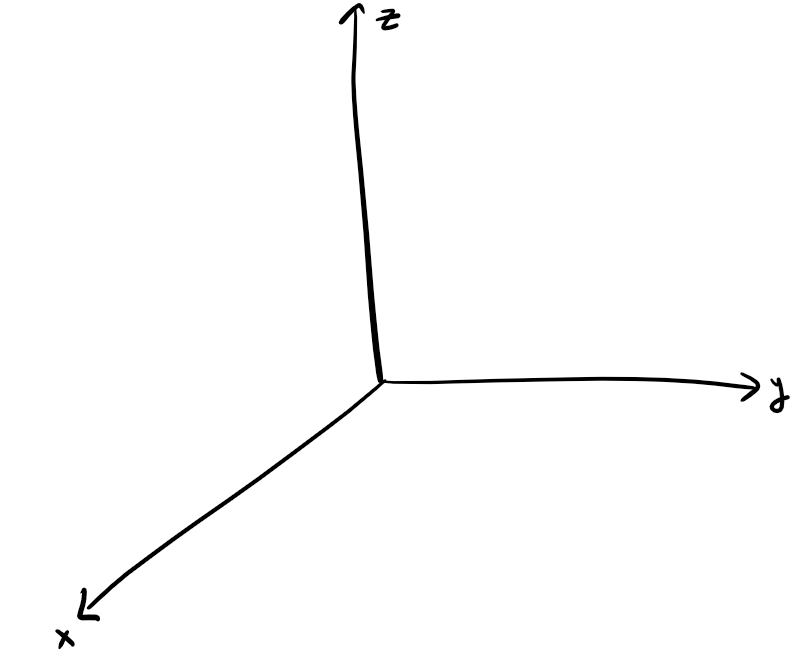
\includegraphics[width=70mm]{Images/coord-axes-R3}
	\caption{Standard labelling of the $x$-, $y$- and $z$-axes of $\mathbf{R}^3$}
	\end{figure}
	\item More generally, $\mathbf{R}^n$ is $n$-dimensional real space. Points are $n$-tuples $(x_1,x_2,\cdots,x_n)$ of real numbers.
\end{itemize}

It's also conceptually useful to write functions in a more formal way. Standard notation for a function $f$ with domain $D$ and range $R$ is written \begin{equation} f\colon D\to R\end{equation} With this notation writing $f\colon \mathbf{R}^3\to\mathbf{R}^2$ means that $f$ is a function whose inputs are triplets $(x,y,z)$, and each such input returns a pair $(p,q)$ of real numbers. It's important to note that $f$ is the function (i.e., the abstract rule which sends a value in $D$ to a value in $R$), the output of the function at a point $P$ in the domain is the value $f(P)$.

\subsection{Vectors in $\mathbf{R}^n$}

A \textbf{vector} $v$ in $\mathbf{R}^n$ is an arrow, starting at the origin, and ending at some point in $\mathbf{R}^n$. It's often convenient to conflate the vector from the origin to a point $P$ with the point $P$ itself. Vectors are written in coordinates by listing the coordinates of the point $P$ at which the vector ends. For instance, the vector $v=(x_1,y_1,z_1)$ is given in figure \ref{fig-vect-P} picture below. 

\begin{figure}[h!] \centering
 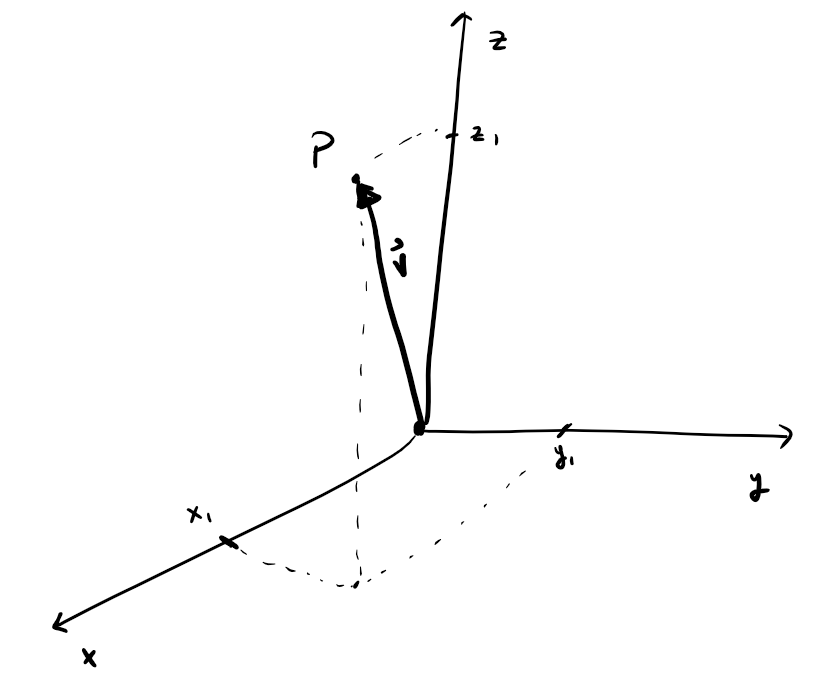
\includegraphics[width=80mm]{Images/vector-P}
 \caption{Vector $v$ as an arrow from the origin to a point $P$ in $\mathbf{R}^3$}
 \label{fig-vect-P}
 \end{figure}

\begin{remark}[Vector notation] You may see notation like $\vec{v}$ to emphasize the $v$ is infact a vector. Similarly, when writing $v$ in components sometimes you will see angled brackets like $\vec{v}=\langle x_1,y_1,z_1\rangle$. This can be useful but is not strictly necessary. I'll write $v$ for a vector and list its coordinates in parentheses most frequently\footnote{If you've taken a course in linear algebra, you may also have familiarity as writing vectors as $n\times 1$ matrices. This is fine, but in the interest of space-efficient typsetting, this will be avoided}. 
\end{remark}

Like numbers, vectors can be \textbf{added} and \textbf{subtracted}\footnote{Multiplication and division is a different story, and is typically not possible to be defined}. Vectors can also be multiplied by \textbf{scalar} quantities\footnote{\textit{Scalar} is just a fancy word for ``non-vector''. Idea being, scalars are what you scale vectors by.}. For a vector $\vec{v}$ and scalar $k$ (i.e., just some real number $k$), $k\vec{v}$ is the vector obtained by rescaling the vector by $\vec{v}$ by the amount $k$. That is to say, if $\vec{u}=(a,b,c)$ and $\vec{v}=(x,y,z)$ are vectors then:
\begin{itemize}
	\item $\vec{u}+\vec{v}=(a,b,c)+(x,y,z)=(a+x,b+y,c+z)$
	\item $\vec{u}-\vec{v}=(a,b,c)-(x,y,z)=(a-x,b-y,c-z)$
	\item $k\vec{v}=k(x,y,z)=(kx,ky,kz)$
\end{itemize}	

Vectors also have a ``zero'' which we denote by $\vec{0}$. In $\mathbf{R}^3$, $\vec{0}=(0,0,0)$ and has the property that \[ {v}+\vec{0}=\vec{0}+{v}={v}\] for all vectors ${v}$. 

\begin{defn}[Norm of a vector] For $v=(v_1,v_2,v_3)$ a vector in $\mathbf{R}^3$, the \textbf{norm} , $|v|$, of $v$ is the scalar quantity given by \begin{equation} |v|=\sqrt{v_1^2+v_2^2+v_3^2}.\end{equation}
\end{defn}

Other words for {norm} include \textit{length} or \textit{magnitude}. If we view $v$ as an arrow in $\mathbf{R}^3$, then $|v|$ is just the length of this arrow, or equivalently the distance from the endpoint of $v$ to the origin. Similar notation is to write $\Vert v \Vert$ for the norm of $v$\footnote{This can be useful to distinguish the \textit{norm} of a vector from the absolute value of a number, but also often leads to a lot of visual clutter. Use whatever you like.}.



\subsection{The dot product} Vectors differ in scalar quantities in that there is typically not a well-defined ``product'' operation like the product of numbers. There are several ``product-like'' operations which we'll use however. Perhaps the most useful is the {dot product}. 

\begin{defn}[Dot product] Given vectors $u=(u_1 ,u_2, u_3)$ and $v=(v_1,v_2,v_3)$ the \textbf{dot product} $u\cdot v$ is defined by \begin{equation} u\cdot v=u_1 v_1+u_2 v_2+u_3 v_3.\end{equation}
\end{defn}

If $u,v$ have more (or fewer) components, the dot product is defined similarly as the sum of the product of corresponding components, you just need that $u,v$ have the same number of components. Sometimes you'll hear the word \textit{inner product} instead of dot product. Note that the dot product $u\cdot v$ is a scalar quantity. The dot product is extremely useful for many things, primarily that the dot product allows us compute the angle between vectors. 

\begin{fact} Let $u,v$ be vectors and  $\theta$ be the angle between\footnote{There are technically two angles between $u$ and $v$, pick the smaller of the two. The angle between vectors will always be in the range of $[0,\pi]$.} them. Then \begin{equation}\label{dot-prod-angle} u\cdot v= |u| |v|\cos \theta.\end{equation}
\end{fact}

In particular, \[\theta=\arccos\left( \dfrac{u\cdot v}{|u||v|}\right)\]
\begin{remark} This tells us a bit about the dot product, for instance if $u,v$ are vectors with angle $\theta$ between them, we have the following (see if you can figure out why this is based off of equation \eqref{dot-prod-angle})
\begin{itemize}
	\item If $0\leq \theta< \pi/2$ then $u\cdot v>0$.
	\item If $\pi/2 < \theta \leq \pi$ then $u\cdot v<0$.
	\item If $\theta=\pi/2$ then $u\cdot v=0$.
\end{itemize}
If $u\cdot v=0$ then we say that $u$ and $v$ are \textbf{orthogonal}. Another word is that $u,v$ are \textbf{perpendicular}\footnote{Orthogonal comes from Greek, perpendicular from Latin, you can choose your own cultural adventure}. It's often very useful to know when vectors are perpendicular, you can think of perpendicular vectors are acting``independently".
\end{remark}

The dot product also gives us the {length} of vectors. Meaning, if $v$ is a vector then: \begin{equation} |v|=\sqrt{v\cdot v}\end{equation}
A convenient way of thinking about the dot product is that allows you to "do geometry" with vectors, i.e., that the dot product allows you to make sense of lengths of and angles between vectors. The dot product exists for vectors in any dimension of real space $\mathbf{R}^n$.

\subsection{The cross product} The \textbf{cross product} is another ``product" of vectors, however it is only defined in the case of vectors in $\mathbf{R}^3$, and lacks a few properties to fully justify it as a ``product". Let's first recall some notation you may have seen in physics. Let's let $\vec{i},\vec{j},\vec{k}$ denote the following vectors\footnote{The use of $i,j,k$ components in physics is part of a longer historical saga than you might realize. The letters specifically come from the \href{https://en.wikipedia.org/wiki/Quaternion}{Quaternions} (or more specifically, the Quaternion algebra), which are a mathematical entity similar to the complex numbers (expect with two other ``complex directions". The cross-product is actually encoded via a multiplication on the vectors $i,j,k$ themselves. This is a very interesting subject, but not something we'll elaborate on much further.}
\[ \vec{i}=(1,0,0), \qquad \vec{j}=(0,1,0), \qquad \vec{k}=(0,0,1)\]
We can then write a vector $v=(a,b,c)$ as a sum of these basis vectors as \[ v=a\vec{i}+b\vec{j}+c\vec{k}\]

\begin{defn}[Cross product] Let $u=(u_1,u_2,u_3)$ and $v=(v_1,v_2,v_3)$  be vectors in $\mathbf{R}^3$. Then the \textbf{cross-product} $u\times v$ of $u$ and $v$ is given by \begin{equation} u\times v= (u_2v_3 - u_3v_2, u_3v_1-u_1v_3, u_1v_2-u_2 v_1).\label{cross-prod-defn}\end{equation}
\end{defn}

Note that the \textit{order} of the terms $u,v$ in the cross product matters. In particular, \[ v\times u=- u \times v\] (see if you can show why based off of \eqref{cross-prod-defn}). Looking at this formula it's maybe not super obvious where this should come from. Let's unpack it. First recall that the determinant of a $2\times 2$ matrix is given by \[ \det\begin{pmatrix} a & b \\ c & d\end{pmatrix} =ad-bc\] The cross product is then calculated by the ``symbolic determinant'' \begin{equation} u\times v= \det \begin{pmatrix} \vec{i} & \vec{j} & \vec{k} \\ u_1 & u_2 & u_3 \\ v_1 & v_2 & v_3 \end{pmatrix} = 
\det\begin{pmatrix} u_2 & u_3 \\ v_2 & v_3 \end{pmatrix} \vec{i} 
- \det \begin{pmatrix} u_1 & u_3 \\ v_1 & v_3 \end{pmatrix} \vec{j} 
+ \det \begin{pmatrix} u_1 & u_2 \\ v_1 & v_2 \end{pmatrix} \vec{k} \end{equation}
You can then check that this is infact the same formula as in \eqref{cross-prod-defn}. Determinants are \textit{everywhere} in mathematics, and we'll see a lot of them throughout this course, so it's useful to internalize the determinant formula of the cross product as your primary means of calculation.

\begin{remark}[Geometric interpretation of the cross product]
Let $u,v$ be two vectors in $\mathbf{R}^3$ that are not parallel (i.e., $u$ is not a scalar multiple of $v$ or vice-versa). Note that there is a unique axis then in $\mathbf{R}^3$ which is perpendicular to both $u$ and $v$. 



The vector $u\times v$ then satisfies the following: 
\begin{itemize}
\item The direction of  $u\times v$ is parallel to this axis, with direction given by the \textit{right-hand rule}\footnote{Take your right hand and point your fingers in the direction of $u$, if you curl your fingers towards $v$ your thumb is the direction of $u\times v$. This gives the ``positive orientation" on 3D space. \href{https://en.wikipedia.org/wiki/Right-hand_rule}{See also} }.
\item The magnitude $|u\times v|$ is the area of the \textit{parallelogram} formed by vectors $u$ and $v$.
\end{itemize}

\begin{figure}[h!]
 \centering 
  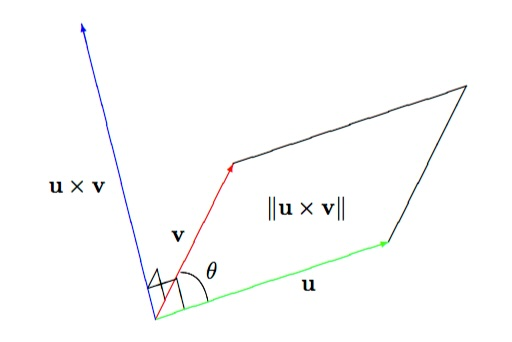
\includegraphics[width=80mm]{Images/cross-prod1} 
   \caption{Cross product of vector $u$ and $v$}
  \label{fig-cp} \end{figure}

Figure \ref{fig-cp} shows geometrically the cross product of $u$ and $v$. In particular, if $\theta$ is the angle between $u$ and $v$ we get that $|u\times v|= |u| |v|\sin \theta$ (I leave it to you to show why the right hand side here is the area of the yellow-shaded parallelogram).\end{remark}



\subsection{Exercises}
\begin{enumerate}[label=\arabic*.]
\item Let $u=(1,2,3)$, $v=(4,-1,1)$ and $w=(1,0,-8)$. 

\begin{enumerate}
	\item Compute the resultant vectors
	\begin{enumerate}[label=(\roman*)]
		\item $u+v+w$
		\item $2u-w$
		\item $3v-4w$
	\end{enumerate}
	
	\item Compute the following norms 
	\begin{enumerate}[label=(\roman*)]
		\item $|u|$
		\item $|u-v|$
		\item $|4w|$
		\item $|-v|$
	\end{enumerate}
\end{enumerate}




\item A \textit{unit vector} is a vector $v$ whose norm $|v|$ is equal to 1. Unit vectors are useful when you want to denote \textit{just} a direction without an influencing magnitude. Find a unit vector in the same direction of each of the following vectors

\begin{enumerate}
	\item $(1,1)$
	\item $(3,4,5)$
	\item $(3,-4)$
\end{enumerate}

\item Use the dot product to find the angle between the two given vectors

\begin{enumerate}
	\item $u=(1,2), v=(-1,-3)$.
	\item $u=(1,1,1), v=(-1,2,-3)$
	\item $u=(1,0), v=(0,1)$
\end{enumerate}

\item Recall that two vectors are \textit{orthogonal} if the angle between them is $\pi/2$. Determine a constant $b$ such that $v=(1,3,5)$ and $u=(-1,1,b)$ are orthogonal, or explain why no such constant exists. 

\item Compute $u\times v$ for the following pairs of vectors $u$ and $v$
\begin{enumerate}
	\item $u=(1,0,2), v=(-3,3,5)$
	\item $u=(-1,1,1), v=(9,0,0)$
	\item $u=i+2j, v=-i+2k$
\end{enumerate}

\item Find a unit vector that is orthogonal to both $u=(1,2,2)$ and $v=(4,4,-7)$

\item Show that $\vec{i}\times \vec{j}=\vec{k}, \; \vec{j}\times \vec{k}=\vec{i}$ and $\vec{k}\times \vec{i}=\vec{j}$. Similarly, show that if $u,v$ are vectors in $\mathbf{R}^3$ that $u\times v=-v\times u$ and $v\times v=0$.
\end{enumerate}

\section{Curves and surfaces} \label{sec-curves-surf}

Before we get into the calculus-based aspects of this course, we need some experience in working with equations of several variables. 

\subsection{Implicit curves in $\mathbf{R}^2$}

You may recall the following (for instance, from learning about implicit differentiation in calc. 1)
\begin{fact} 
Any equation in the variables $x$ and $y$ describes a curve $C$ in the $xy$-plane
\end{fact}

For example, the equation $x^2+y^2=1$ describes the unit circle in the $xy$-plane, with radius $1$ and center $(0,0)$. Similarly, $y=2x-1$ is a line with slope $2$ and $y$-intercept $-1$. 

\begin{remark} It's useful to really nail down what is happening here: when we say ``...$x^2+y^2=1$ describes the unit circle..." what this really means is that the unit circle in $\mathbf{R}^2$ is the collection of all points $(x,y)$ in $\mathbf{R}^2$ such that $x^2+y^2=1$. Sometimes you'll see this written in \textit{set-builder notation} as \[ \{ (x,y) : x^2+y^2=1\}\]  \end{remark}


Note that any equation of two variables can be written in the form $F(x,y)=0$ for some two variable\footnote{Technically we haven't defined what a two variable function is, but I think you can work with it. See Section \ref{multivar-function}} function $F$. We say that this is an \textbf{implicit description} of the curve $C$ described by that equation. Similar terminology is to say that  $C$ is an \textbf{implicit curve} or that $F(x,y)=0$ is an \textbf{implicit function} describing $C$. It can be typically very difficult to determine the shape of an implicit curve is, even if the function $F$ feels friendly.

\subsection{Implicit surfaces in $\mathbf{R}^3$}
We begin with a similar fact to the previous case. 

\begin{fact}
Any equation in the variables $x$, $y$ and $z$ describes a surface $S$ in the $xyz$-space.
\end{fact}

Here, \textit{surface} simply means ``$2$-dimensional thing" living inside $\mathbf{R}^3$. If the equation is rearranged to the form $F(x,y,z)=0$ for some three variable function $F$ we say that $F$ \textbf{implicitly defines} the surface $S$, or that $F(x,y,z)=0$ is an \textbf{implicit function} defining $S$). 
 
\begin{example}These types of objects are probably new, and we'll compile a good reference list for some commonly used surfaces. Surfaces can be as (and often more) difficult as curves, so your expectation should be that these are typically ``complicated" objects. Some examples: \begin{itemize}
	\item $x^2+y^2+z^2=1$ is the unit sphere
	\item $x+y+z=1$ is a plane that passes through points $(1,0,0), (0,1,0)$ and $(0,0,1)$
	\item $z=x^2+y^2$ is a \textit{paraboloid}, i.e., the surface obtained by rotation the graph $z=x^2$ (in the $xz$-plane) about the $z$-axis (in $\mathbf{R}^3$)
\end{itemize}
Recall just as before that writing such an equation is asking for all points $(x,y,z)$ in $\mathbf{R}^3$ that satisfy the given equation. 

\subsection{Systems of equations}
Given a collection of equations (say of variables $x,y,z$), a solution to \textit{all} equations at once can be thought of geometrically as a point which lies on all of the implicit surfaces defined by those equations. 

The thing to note is the basic idea that\begin{align*} \text{One equation of variables $x,y,z$} \quad &\iff \quad \text{A surface in $\mathbf{R}^3$}  \\ 
\text{Two equations of variables $x,y,z$} \quad & \iff \quad \text{Intersection of two surfaces in $\mathbf{R}^3$}\\
\text{Three equations of variables $x,y,z$} \quad & \iff \quad \text{Intersection of three surfaces in $\mathbf{R}^3$, \quad etc.}
\end{align*}
\end{example}

Generally, when you intersect a pair of surfaces you expect to get a curve out. If you intersect three surfaces with each other, you expect a bunch of points (i.e., $0$-dimensional things). Said differently, by intersecting things that have dimension, the dimension goes down. This is not always the case, and requires that the surfaces are ``independent", but is a good rule of thumb.
 
\begin{remark}
Sometimes your equations will result in the ``empty curve'' or ``empty surface"---meaning, that there are no points that satisfy the given equation. For definitional clarity, we should accept this as okay. For instance, $x^2+y^2=-9$ has no solutions in $\mathbf{R}^2$, and thus defines the empty curve (that is, the curve which has no points on it).
\end{remark}

\subsection{Planes} 
A \textbf{plane} is a flat surface in $\mathbf{R}^3$. What does this mean? First, note that the notion of ``slope'' doesn't quite make sense here\footnote{At the least, you would need slopes $z$ with respect to $x$ and separately with respect to $y$.}, rather what we use to denote the direction of a surface is a \textbf{normal vector}. 
\begin{defn}[Normal vector]
Given a surface $S$ and point $P$ on the surface, we say that a vector $\vec{n}$ is a \textbf{normal vector} to $S$ if $\vec{n}$ is perpendicular to the surface at $P$.
\end{defn}
You might have objections to this definition at the moment (i.e., what does perpendicular mean here?\footnote{We'll answer this better once we understand the \textit{tangent plane} to a surface, see Section \ref{sec-tan-plane}.}), but let's see how this works for a plane. Planes are exactly those surfaces whose normal vectors are the same at all points on the surface. To create the equation which defines a plane we may be interested in, we'll typically use the following: 
\begin{defn}[Plane builder notation] Given a point $P=(a,b,c)$ and normal vector $\vec{n}=(u,v,w)$, the plane through $P$ with normal vector $\vec{n}$ is given by:
\begin{equation} \label{plane-creator} \vec{n} \cdot (x-a,y-b,z-c)=0\end{equation}
\end{defn} 
You can think of this analogously to \textit{point-slope form} for lines in $\mathbf{R}^2$. In words, this equation \eqref{plane-creator} is looking for all points $(x,y,z)$ in $\mathbf{R}^3$ such that the displacement vector $v$ from $P$ to $(x,y,z)$ is perpendicular to $\vec{n}$ (see figure \ref{fig-plane} below). \begin{figure}[h!] \centering
 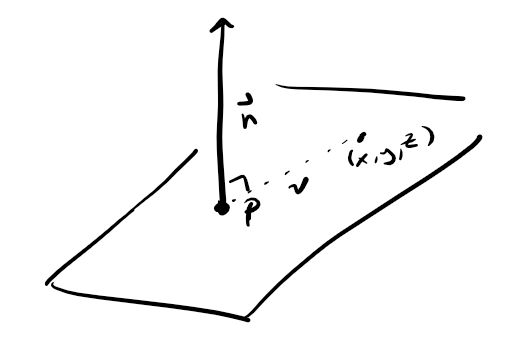
\includegraphics[width=70mm]{Images/plane-normal} 
  \caption{Plane with normal vector $\vec{n}$ through point $P$}
  \label{fig-plane}
\end{figure}

\begin{remark} Unraveled, all planes are given by \textit{linear} equations in the variables $x,y,z$: i.e., \begin{equation} \label{plane-eqn} u x+v y+w z=k \end{equation} for some constants $u,v,w,k$. In particular, if you are given the equation \eqref{plane-eqn} for some plane, then this plane has normal vector given by $\vec{n}=(u,v,w)$.\end{remark}

\subsection{Quadric surfaces}
In learning basic planar geometry, we know that lines are the simplest types of objects, followed by quadratic equations (i.e., parabolas or ellipses\footnote{If you know your conic sections, these are exactly the shapes that are described by quadratic equations: parabola, circle, ellipse, and hyperboloid}). Going up a dimension, the next simplest types of surfaces beyond planes should be those whose defining equation is a quadratic polynomial. These are called \textbf{Quadric surfaces} (you can also say \textit{quadratic surface}, but that's not quite right). 

\begin{example}Some examples of quadric surfaces are given below (here $k$ is some constant)

\begin{itemize}
	\item $x^2+y^2+z^2=k^2$ is a \textbf{sphere} of radius $k>0$ centered at the origin.
	\item $x^2/a^2+y^2/b^2+z^2/c^2=1$ for constants $a,b,c$ is an \textbf{ellipsoid}. The constants $a,b,c$ should all be positive, they represent the ``radius" of the ellipsoid in the $x$-, $y$-, and $z$-axes respectively.
	\item $z=x^2+y^2$ is a \textbf{paraboloid} (also called \textbf{elliptic paraboloid} opening in the upward $z$-direction
	\item $z=x^2-y^2$ is a \textbf{saddle point} (also called a \textbf{hyperbolic paraboloid}) this is the shape of a Pringle
	\item $z^2=x^2+y^2$ is a \textbf{cone} (opening along the $z$-axis)
	\item $x^2+y^2=k^2$ (as an equation of the variables $x,y,z$) is a \textbf{cylinder} (with tube-y part going along the $z$-axis)
	\item $y=ax^2+k$ ($a,k$ constants) is a \textbf{parabolic sheet} (also called a \textbf{parabolic cylinder}), i.e., the parabola $y=ax^2+k$ extended indefinitely in the $z$-direction
	\item $x^2+y^2-z^2=k$ is a \textbf{hyperboloid} (if $k>0$ it is a hyperboloid of one sheet\footnote{This is also the shape of a nuclear cooling silo}, if $k<0$ it is a hyperboloid of two sheets). 
\end{itemize}
See below for some pictures 
\begin{figure}[h!]
\centering
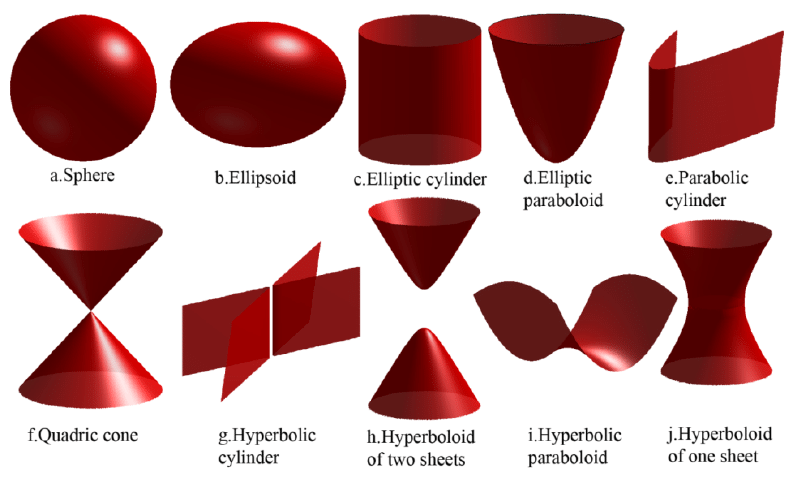
\includegraphics[width=150mm]{Images/quadrics}
\caption{Some examples of quadric surfaces}
\label{fig-quadrics}
\end{figure}

Your usual graph transformations can be applied to translate or stretch/shrink these basic shapes. For instance, $(x-4)^2+(y+1)+z^2=9$ is a sphere of radius $3$ centered at $(4,-1,0)$. With a little bit of effort (i.e., completing the square) you can take \textit{any} quadratic equation of the variables $x,y,z$ and translate it into one of the examples above.

\end{example}

Throughout the term we will make frequent use of these types of surfaces, so it's good to familiarize yourself with what equation goes to what shape. 

\subsection{Exercises}

\begin{enumerate}[label=\arabic*.]
	\item Write an equation for each of the following planes
	\begin{enumerate}
		\item The plane through $(0,0,1)$ with normal vector $(1,3,2)$
		\item The plane through points $(3,2,1)$, $(1,0,-1)$ and $(4,-1,5)$
		\item The plane through the origin which contains the two vectors $v=(1,2,3)$ and $u=(-1,2,-1)$
	\end{enumerate}	
	
	
	\item Determine the type of quadric surface formed by each of the following equations. Give as much information about the surface as you can.
	\begin{enumerate}
		\item $x^2+3y^2+z^2=10$
		\item $z^2-10y^2=1$
		\item $x^2+y=1-z$
		\item $3y^2+3z^2=1$
		\item $x^2-y^2+2z^2=-4$
		\item $3x^2+3y^2=z^2$
		\item $x^2-2x+y^2-6y+z^2=9$ \quad (\textit{Hint: complete the squares in $x$ and $y$})
	\end{enumerate}

	\item \textit{True or False}. Determine if the following statements are true or false. Give a brief justification of your answer.
	\begin{enumerate}
		\item  $\vec{n}=(1,3,1)$ is a normal vector to the plane $x+3y=4-z$\
		\item $x^2+y^2=z^4+4z$ is a quadric surface
		\item There are no points $(x,y,z)$ which satisfy $x^2+y^2+z^2=-10$
		\item The intersection on two planes always forms a line
		\item The intersection of two spheres always forms a circle
	\end{enumerate}
	
	\item Let $(x_1,y_1,z_1), (x_2, y_2, z_2), (x_3, y_3, z_3)$ be three points in $\mathbf{R}^3$. Show that the plane through these three points is given by the equation \[ \det \begin{pmatrix} x-x_1 & y-y_1 & z-z_1 \\ x_2-x_1 & y_2-y_1 & z_2-z_1 \\ x_3-x_1 & y_3-y_1 & z_3-z_1\end{pmatrix} = 0 \]
\end{enumerate}



\section{Parametric curves}
\label{sec-param}

A loose definition is that a \textit{curve} is a 1 dimensional \textit{thing} that lives in $\mathbf{R}^n$. In the last section, we gave implicit descriptions for curves in $\mathbf{R}^2$, but made no mention of curves in $\mathbf{R}^3$ or higher. What gives? The problem is that to describe a curve in $\mathbf{R}^3$, you need two equations\footnote{Generally, a collection of $k$ equations in $n$ variables will be an $(n-k)$-dimensional thing in $\mathbf{R}^n$}. When discussing curves, we often want something stronger than an implicit description, however. This gets us to the idea of a \textit{parametrized} curve. 

\begin{defn} A \textbf{parametric curve} in $\mathbf{R}^3$ is a function $\vec{r}\colon \mathbf{R}\to \mathbf{R}^3$ of the form \begin{equation} \vec{r}(t)=(x(t),y(t),z(t)) \end{equation}  \end{defn} 
The functions $x(t),y(t),z(t)$ are called the \textit{component functions} of $\vec{r}$. When convenient, we'll drop the arrow and just write $r$ for $\vec{r}$. Sometimes you'll also see \textbf{vector-valued function} used to describe this type of object. There is of course a similar definition of a parametric curve in $\mathbf{R}^2$, omitting the $z$ coordinate in the description above. The domain of a parametric curve need not be the entirety of $\mathbf{R}$, often we'll want to specify an interval as the domain. 

\begin{remark}The word \textit{parametric} comes from the idea that we are describing the coordinates (i.e., location) of a particle in terms of a new \textit{parameter} (in this case $t$). It's compelling and often sufficient to think of $t$ as time, in which case the parametric curve gives a description of the movement of this particle in 3D space. \end{remark}

\subsection{Trajectories}
The \textbf{trajectory} of a parametric curve is the image of the path taken by the parametrization. This is what we can talk about when we write down a bunch of equations which describes this curve. The trajectory of a parametric curve is what we otherwise may just call a \textit{curve} (see Section \ref{sec-curves-surf}), and we'll write $C$ for such an object. Generally, many parametrizations exist of the same trajectory. 


\begin{example}[Parametrization of a line]
A \textbf{line} is the simplest type of curve that we can have. A line has two pieces of information: A point $P$ on the line, and a direction vector $\vec{v}$. With this set up we can parametrize the line through $P$ in direction $\vec{v}$ as \begin{equation} \vec{r}(t)=P+t\vec{v}\end{equation}
More specifically, if $P=(a,b,c)$ and $\vec{v}=(v_1,v_2,v_3)$ then this line is parametrized as \[ \vec{r}(t)=(a,b,c)+t(v_1,v_2,v_3)=(a+tv_1,b+tv_2, c+tv_3)\] 
Note that each component of the parametric function is \textit{linear} in the variable $t$. 
\end{example}

\subsection{Tangent vectors} 

Given a parametric curve $\vec{r}(t)=(x(t),y(t),z(t))$ such that the coordinate functions are differentiable we can talk about the \textbf{tangent vector} to this curve. Define the tangent vector by \begin{equation} \vec{r}\,'(t)=(x'(t),y'(t),z'(t))\end{equation} where $'$ denotes derivative with respect to $t$. Since this is a vector is has a norm and a direction. They contain the respective information \begin{itemize}
	\item The direction of $\vec{r}\,'$ indicates the \textit{direction of instantaneous travel} of $\vec{r}$ 
	\item The norm $|\vec{r}\,'|$ indicates the \textbf{speed} of the parametrization
\end{itemize}
If you think of $r$ as parameterizing the motion of a particle in space, then $\vec{r}\,'$ is just the velocity vector. It's often useful to define \begin{equation} s(t)=|\vec{r}\,'(t)|\end{equation} to be the \textbf{speed function} associated to a parametrization $\vec{r}$.

\subsection{Smoothness} \label{sec-smooth}
Since we have defined the tangent vector to a curve it's useful to talk about when this tangent vector does not have enough information to give either a well-defined speed or direction to the curve. These points are called cusps as defined below.

\begin{defn}[Cusp] Given a parametric curve $\vec{r}(t)=(x(t),y(t),z(t))$, we say that $\vec{r}$ has a \textbf{cusp} at $t=t_0$ if either $\vec{r}\,'(t_0)=(0,0,0)$ or $\vec{r}\,'(t_0)$ does not exist. \end{defn}

If a parametric curve has no cusps on its domain then it is called \textbf{smooth}. Note that equivalently a parametrization is smooth if the speed function $s$ is defined and satisfies $s(t)>0$ for all $t$ in the domain of $\vec{r}$. Smooth curves are the ones which make sense for us in terms of calculus.

\begin{remark}
This last section has been written for parametrized curves in $\mathbf{R}^3$, but there's absolutely nothing special about dimension 3 here. The terminology and expressions work just as well in any $\mathbf{R}^n$.
\end{remark}

\subsection{Exercises} 
\begin{enumerate}[label=\arabic*.]
\item Sketch or otherwise determine the trajectory of the following curves

\begin{enumerate}
	\item $r(t)=(2, t)$
	\item $r(t)=(\cos(t)+1, \sin(t)-2)$
	\item $r(t)=(t,t^2,1)$
	\item $r(t)=(t^2, t, \sin(t))$

\end{enumerate}

\item Sketch the projections of $r(t)=(t^2,t^3, t^{-3})$ to the three coordinate planes. Use these graphics to attempt to sketch the graph of $r(t)$.



\item Give a parametric description of the following lines

\begin{enumerate}
	\item The line starting at $(1,2,3)$ pointed in the direction $(-1,0,1)$.
	\item The line starting at $(-1,2,2)$ pointed towards $(1,1,1)$. 
	\item The line $x=y+2$ viewed in 3 dimensional space as lying in the $xy$-plane
\end{enumerate}



\item Determine any points where the line $x=t,y=t,z=-t$ intersects the plane $3x-2y+5z=4$.

\item Show that $r(t)=(t\cos t, t\sin t, t)$ lies on the cone $z^2=x^2+y^2$. Can you sketch the graph of $r(t)$?

\item Parametrize the line of intersection of the planes $2x-y-z=-1$ and $x+3y+2z=2$. Do the same for $x+y=1$ and $y+z=1$. (\textit{hint: the direction of this line is perpendicular to the normal vectors of both planes}).


\item Two particles are moving according to vector functions $r_1(t)=(t,t^2,t^3)$ and $r_2(t)=(1+2t, 1+6t, 1+14t)$. Determine any points where the particles collide. Determine any points where the \textit{trajectories} of the particles collide. (\textit{hint: these two questions are not the same.}) 

\item Parametrize the intersection the cylinder $x^2+y^2=4$ and surface $z=xy$ as a vector-valued function $r(t)$. Do the same for  the paraboloid $z=4x^2+y^2$ and surface $y=x^2$.


\item Determine the tangent vector $r'(t)$ for each of the following curves $r(t)$; use this to find any cusps of the parametrized curves. 

\begin{enumerate}
	\item $r(t)=(e^t, t^3-2, \ln t)$
	\item $r(t)=(\sqrt{t-2}, 1/t^2)$
	\item $r(t)=(t^2+1, 1-t^2, 4)$
	\item $r(t)=\left(\dfrac{1}{1+t}, \dfrac{t}{1+t}\right)$
\end{enumerate}

%\item Find the \textit{unit} tangent vector to the $r(t)=(\cos t, 3t, \sin (2t))$. Do the same for $(e^t, e^{2t}, e^{3t})$.

\item Show that $r_1(t)=(t, t^2, t^3)$ and $r_2(t)=(\sin t, \sin(2t), t)$ both pass through the origin at $t=0$. Use this to find the angle at which these curves intersect. (\textit{Find the tangent vectors to $r_1$ and $r_2$ when $t=0$ and use the dot product to find the angle between these vectors}.)


\item \label{dot-derivative} Suppose that $r_1(t)$ and $r_2(t)$ are both vector-valued functions landing in 3 dimensional real space. Derive formulas for \[ \dfrac{d}{dt} (r_1(t)\cdot r_2(t)) \text{\quad and \quad }\dfrac{d}{dt} (r_1(t) \times r_2(t))\] in terms of $r_1, r_2$ and their tangent vectors. 

\item Show that if $|r(t)|$ is constant, then $r(t)\cdot r'(t)=0$--i.e., $r(t)$ and $r'(t)$ are orthogonal. (\textit{Hint: Use problem \ref{dot-derivative} to differentiate $|r(t)|^2=r(t)\cdot r(t)$.}) \label{tan-to-derivative}

\item \textit{True or false}. Determine if the following statements are true or false. Give a brief justification of your answer

\begin{enumerate}
	\item The line between points $P$ and $Q$ in 3-dimensional space can be parametrized as $r(t)=P+(Q-P)t$.
	\item The line between points $P$ and $Q$ in 3-dimensional space can be parametrized as $r(t)=Q+(P-Q)t$.
	\item The trajectory of $r(t)=( \cos t, -t, \sin t)$ lies on the cylinder $x^2+y^2=1$. 
	\item The trajectory of $r(t)=(t^2,-2t^2)$ lies on the graph $y=-2x$.
\end{enumerate}
\end{enumerate}

Suggested additional exercises. \textit{Stewart} sections 13.1, 13.2



\section{Arclength of smooth curves}


This section concerns describing the ``length'' of curves, aptly called \textit{arclength} (as in length of the arc). Suppose we have a curve parametrized by the vector function $r=r(t)$ for $t$ in some interval $[a,b]$. % us call the \textbf{trajectory} (i.e., the path that we see) by $C$. Note that many different vector functions $r(t)$ can parametrize the same trajectory.
Recall that a parametrization is smooth if $|r'(t)|\neq 0$ for all $t$. Note that is to say the \textit{speed} vector of this curve is always nonzero\footnote{I encourage you to think of the ways the velocity of a curve could be the zero vector: one is if the trajectory $C$ has a sharp turn---\textit{cusp} in the language of differentiable calculus---but this is not all possible instances. The given parametrization could also ``stop'' at some point.}.  Similarly, we say a given trajectory $C$ is \textbf{smooth} if it can be parametrized by a smooth vector function.

\begin{defn}[Arclength] Let $C$ be a smooth curve with parametrization $r(t)$ for $t$ in some interval $[a,b]$. The \textit{arclength} of $C$ is given as  
\begin{equation} \label{arc-length}
	L = \int_a^b |r'(t)| \,dt
\end{equation}
\end{defn}
The equation \eqref{arc-length} can be best understood as saying length (i.e., distance) is given by speed over time. However, when you have a varying speed, the correct interpretation of ``over time'' is to integrate the speed function: if the speed is constant, then $L=$ speed $\times$ time recovers the classic formula from physics. 

Note if $r(t)=(x(t), y(t))$ is a parametric curve in $\mathbf{R}^2$ then \eqref{arc-length} becomes \begin{equation} L = \int_a^b \sqrt{x'(t)^2 +y'(t)^2}\,dt\end{equation} which may look familiar from previous courses. The benefit of \eqref{arc-length} however is that there is no mention of the dimension where the curve lives (and therefore that formula will work in any space $\mathbf{R}^n$). 

Of all possible parametrization the ``best'' one is the one which satisfies $|r'(t)|=1$ for all $t$. In this case, the arclength of $C$ is just the length of time interval it is defined on, i.e., $L=b-a$. We say that a parametric curve $r(t)$ is \textbf{parametrized by arclength} if \begin{equation} |r'(t)|=1 \qquad \text{ for all $t$ in the domain of $r$} \end{equation}  Notation-wise, we usually use $s$ (instead of $t$) for the input variable of an arclength parametrization of $C$. We'll see shortly some benefits of having a parametrization by arclength. 
 
\subsection{Exercises} 
 
 \begin{enumerate}[label=\arabic*.]
\item Find the arclength of the following curves on the given time intervals
\begin{enumerate}
	\item $r(t)=(2t, 3+t, t)$, $0\leq t\leq 10$
	\item $r(t)=(\cos^3t,\sin^3 t,2)$, $0\leq t\leq \pi/2$
	\item $r(t)=(e^t, e^{-t}, \sqrt{2}t)$, $0\leq t\leq 1$
\end{enumerate}

\item Determine if the following curves are parametrized by arclength (i.e., if $|r'(t)|=1$ for all $t$)

\begin{enumerate}	
	\item $r(t)=(t,t,t)$
	\item $r(t)=(e^t, e^{-t})$
	\item $r(t)=(\cos(2t)/2, \sin(2t)/2)$
\end{enumerate}


\item Consider the parametric function $r(t)=(1+t, 3-2t, 4+2t)$.

\begin{enumerate}
	\item Show that $|r'(t)|=c$ where $c$ is a constant not equal to $1$.
	\item Explain why the substitution $t=s/c$ (where $c$ is the constant from part a.) reparametrizes the curve by arclength (i.e., $|r'(s)|=1$ for all $s$).
\end{enumerate}


\item Let $r(t)=(t^3/3, t^2/2)$ for $t\geq 0$. 

\begin{enumerate}
	\item Show that $r(t)$ is not parametrized by arclength
	\item Determine a reparametrization of $r(t)$ which is parametrized by arclength by the following steps
		\begin{enumerate}[label=\roman*.]
			\item Find arclength  $s=\displaystyle \int_0^{t} |r'(\xi)|\, d\xi$ as a function $s$ in terms of time $t$
			\item Determine the inverse of this function, i.e., $t$ in terms of $s$
			\item Substitute this inverse into the description of $r(t)$ to obtain $r(s)$ parametrized by arclength
		\end{enumerate}
\end{enumerate}

\item Show that if $y=f(x)$ is the graph of a differentiable function $f$ with domain $[a,b]$, then the arclength of the graph is given by \begin{equation} \int_a^b \sqrt{1+f'(x)^2}\,dx\end{equation}
Use the above formula to find the arclength of the parabola $y=x^2$ defined on $[0,1]$ (\textit{Hint: you might want to lookup $\displaystyle \int \sec^3\theta\,d \theta$.}) 

\item \textit{True or False}. If $C$ is a smooth curve and $r(t)$ is a given parametrization of $C$, then $r(t)$ is a smooth vector function. 
\end{enumerate}

Suggested additional exercises. \textit{Stewart} Section 13.3 

\section[Curvature]{Unit tangent and normal vectors, curvature, and torsion} \label{sec-curvature}

When studying the geometry of curves, it becomes useful to often just ask of the direction the curve is pointing at a given time. In formulas, this would mean eliminating any information about \textit{speed} of a parametrization. 

\subsection{The $T$, $N$, $B$ frame}
\begin{defn}[Unit tangent vector]Let $r(t)$ be a parametrization of a smooth curve. The \textbf{unit tangent vector} $T(t)$ is the vector function \begin{equation} \label{unit-tangent} T(t)= \dfrac{r'(t)}{|r'(t)|} \end{equation}
\end{defn}

Note  since $r(t)$ is smooth that $|r'(t)|\neq 0$. Any vector function whose output is always a unit vector has the following property (see Exercise \ref{tan-to-derivative} in Section \ref{sec-param}). 
\begin{fact} If $r$ is any parametrization such that $|r(t)|=1$ for all $t$, then $r(t)$ and $r'(t)$ are orthogonal\end{fact} 
Applying this fact to the vector function $T(t)$ we get a well-defined perpendicular direction to $T$ (and thus also $r'$). This is called the \textbf{principle normal direction} of the curve. Since this direction depends on the time derivative of the tangent direction, the principle normal direction (if it exists) points in the direction in which the curve is bending. 

\begin{figure}[h!]
\centering
 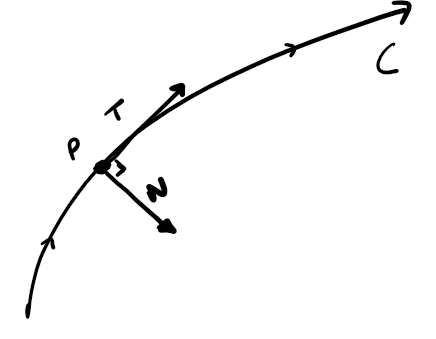
\includegraphics[width=60mm]{Images/curve-TN}
 \caption{Unit tangent $T$ and unit normal $N$ vectors for a parametrized curve $C$} 
 \end{figure}
 
\begin{defn}[Unit normal vector] Let $r(t)$ be a parametrization of a smooth curve and $T(t)$ its unit tangent vector. The \textbf{unit normal vector} $N(t)$ is the vector function \begin{equation} \label{unit-normal} N(t)=\dfrac{T'(t)}{|T'(t)|} \end{equation}
\end{defn}
%Note that $N(t)$ and $T(t)$ are always perpendicular. It's often quite a pain to compute $N(t)$ but it does tell us useful information about which direction a curve is ``bending'', more on this to come. 


\begin{remark}[Binormal vector]If $r(t)$ parametrizes a curve in $\mathbf{R}^3$, it's customary to define the \textbf{binormal vector} $B$ by  \begin{equation} 
	B(t)=T(t)\times N(t)
\end{equation} for all $t$. Since $T,N$ are perpendicular unit vectors, $B$ is then a unit vector perpendicular to both $T$ and $N$ (why?). While it may seem odd at the moment, this $T,N, B$ ``frame'' gives you a consistent choice of coordinates (i.e., $x,y,z$) for position \textit{relative} to an object moving in space. This is sometimes useful in physics when talking about reference frames. The benefit is that $T,N$ and $B$ are uniquely and canonically formed just from the information of the parametrization $r(t)$. Math3D has a \href{https://www.math3d.org/tnb}{useful interface} for visualizing this frame move throughout 3d-space. 
\end{remark}

\subsection{Curvature} Curvature is a way of specifying the exact amount that a given parametric curve is ``curved''. As with anything in math, this notion should agree with our intuition about what sort of things are curved and what are not. A noncontroversial take is that curvature should obey the following properties: 
\begin{itemize}
	\item A straight line is not curved
	\item A circle is curved, and the curvature of a circle depends on its radius 
\end{itemize}



We can use this idea to define curvature for an arbitrary curve as follows. Given a smooth curve $C$ and point $P$ on the curve, compute the radius of the ``best approximating\footnote{It's tempting to say  \textit{tangent} here, but just asking that we find a circle whose tangent line matches that of the curve does not uniquely describe this circle (why?). What you really need to do to calculate this is use the following idea: a circle is determined by three points in the plane. Fix one at $P$, pick two others (say one on each side of $P$) which lie on the curve, and find the circle through these three points. Then compute the ``limiting circle" you get as the two other points tend to $P$. This is not particularly easy to do.} circle'' to the curve at the given point on this curve. That is, find the radius of the circle which best fits inside the curve at a particular point. 

\begin{figure}[h!]
\centering
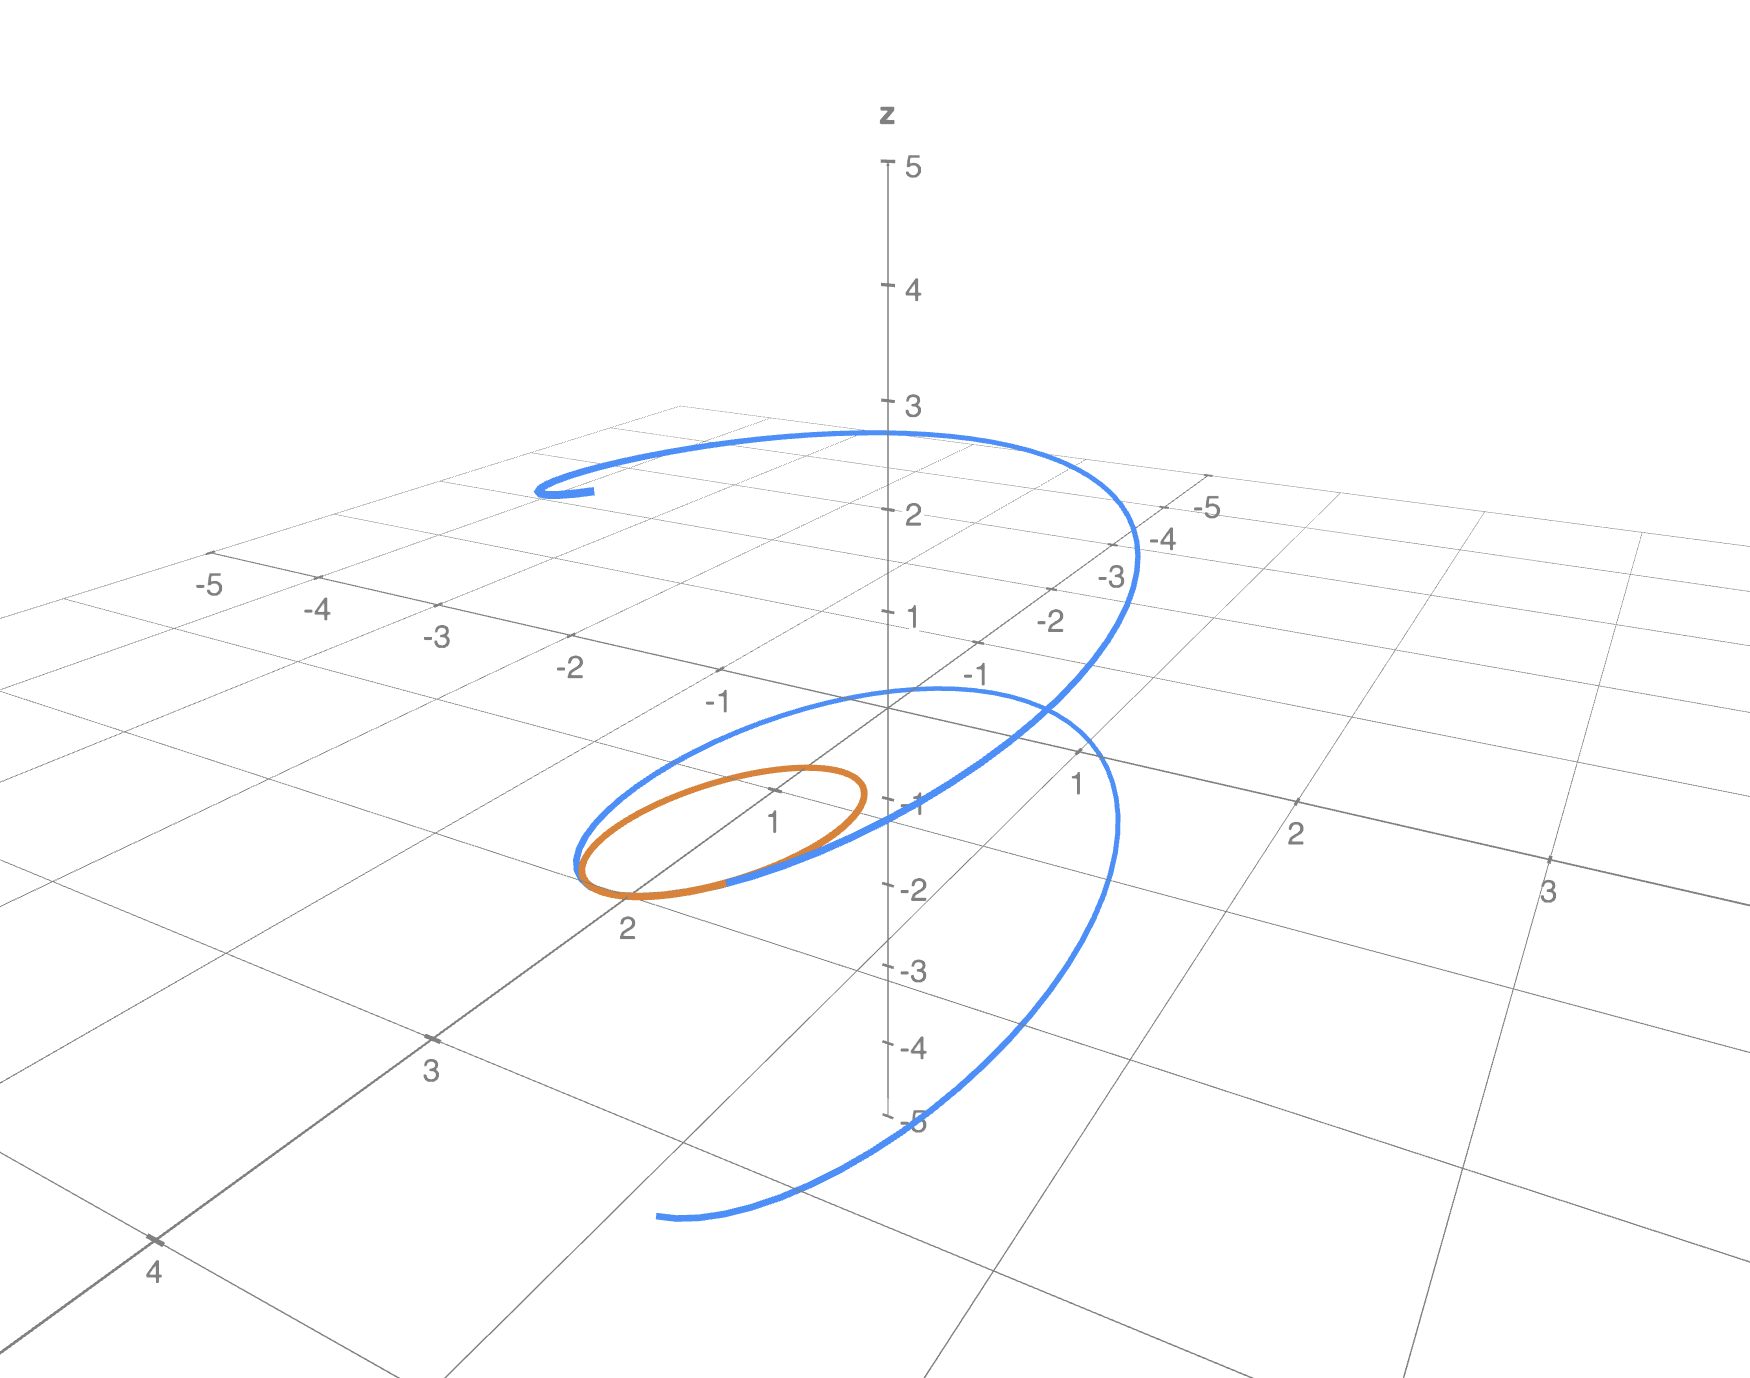
\includegraphics[width=80mm]{Images/curvature-pic}
\caption{The osculating circle (orange) for a smooth curve (blue)}
\label{fig-osc-circle}
\end{figure}

If this circle exists it's called the \textbf{osculating circle}\footnote{\textit{Osculating} is evidently latin for ``kissing", which is really just a synonym for tangent.}. A picture is given in Figure \ref{fig-osc-circle} (Math3D also has a \href{https://www.math3d.org/osculating_circle}{useful tool} for visualizing how this osculating circle changes as you move along the curve)



\begin{defn}[Curvature] Let $C$ be a smooth curve and $P$ a point on $C$. If the osculating circle to $C$ at point $P$ exists and has radius $R$, the \textbf{curvature} of $C$ at point $P$ is defined to be $1/R$.
\end{defn} 

Notation wise, we use $\kappa$\footnote{This is the Greek letter ``kappa'' not a $k$} to denote curvature. If $C$ has a parametrization by $r(t)$, then we can define the curvature function $\kappa(t)$ which at a value $t=t_0$ tells us the curvature at the point $r(t_0)$ on $C$. 

Note as $R\to \infty$, that $1/R\to 0$, thus the curvature of a straight line is 0. Similarly, any circle of radius $R$ has curvature $1/R$. This definition of curvature is not particularly easy to compute, however. The following allows us to calculate curvature using the unit tangent vector $T$: 

\begin{thm} Let $C$ be a smooth curve parametrized by $r(t)$, and $T(t)$ be its unit tangent vector.  The curvature function $\kappa(t)$ of $C$ is given by \begin{equation} \label{c1}
	\kappa(t) = \dfrac{|T'(t)|}{|r'(t)|}
\end{equation}
\end{thm}

In words, curvature is just the ratio of how fast a curve is changing its direction relative to the speed of the curve. This gives us a measure of how much a curve is ``bending'' inwards at a given point (curvature is always in the direction of the unit normal vector $N(t)$.) 

It's worth pointing out that curvature is a feature of the \textit{curve} and not of a particular parametrization of it, that is to say, equation \eqref{c1} will give you the same curvature at a given point on the curve, even if different parametrizations are used. 

\begin{remark}[Other formulas for curvature]While \eqref{c1} gives us a good definition of curvature, it can often be difficult to explicitly write a the unit tangent vector of a curve. The two following equations offer alternative computations for curvature which are often somewhat easier. \begin{equation} \label{c2}
	\kappa(t)= \dfrac{ |r'(t) \times r''(t)| }{|r'(t)|^3} \end{equation}

In the specific case that we have a curve that is the graph of a function $y=f(x)$ in the $xy$-plane, curvature can be defined as follows \begin{equation} \label{c3}
	\kappa(x)=\dfrac{|f''(x)|}{\left(1+(f'(x))^2\right)^{3/2}} \end{equation} 
Showing that these formulas are valid is tricky, but doable. We'll focus on using these defining equations to do some spiffy things. \end{remark}

\subsection{Torsion} For planar curves, knowing the curvature of the curve is essentially enough information to reconstruct the whole curve (you need to know a starting point, and probably want the curvature to be \textit{signed}, but let's not worry about that). For curves which live in $\mathbf{R}^3$, this is no longer true: for instance, both circles and helixes have constant curvature but are by no means the ``same" curve. 

What further distinguishes space curves, is \textit{torsion}. This is a number which signals the amount which $C$ ``lifts'' out of the plane spanned by the tangent and normal vectors (sometimes called the \textit{osculating plane} at a given point on the curve. 
\begin{defn}[Torsion] Given a smooth smooth curve $C$ in $\mathbf{R}^3$ parametrized by $r(t)$, the \textbf{torsion} $\tau$ of $C$ as a function of $t$ is calculated by \begin{equation} \label{t1} 
	\tau(t)=- \dfrac{B'(t)\cdot N(t)}{|r'(t)|}\end{equation}
\end{defn}
It's not particularly clear that this formula should do what we described above, nor is the calculation of torsion necessarily an easy one. An equivalent definition is that \begin{equation} \tau(t)= \dfrac{ (r'(t) \times r''(t)) \cdot r'''(t)}{|r'(t)\times r''(t)|^2}\end{equation}
but this still is not particularly easy to calculate except in some nice cases.

A neat fact then is that a smooth space curve is uniquely determined by the following information: (i) A starting point, (ii) its curvature, (iii) its torsion (see also the  \href{https://en.wikipedia.org/wiki/Frenet\%E2\%80\%93Serret_formulas}{Fresnel-Serret formulas})

\subsection{Exercises}
\begin{enumerate}[label=\arabic*.]
\item Compute the unit tangent vector $T(t)$ and unit normal vector $N(t)$ for the given parametric functions at the indicated time of $t$. If you're feeling strong, compute $B(t)$ as well.

\begin{enumerate} 
	\item $r(t)=(t^2-1, t)$, $t=1$
	\item $r(t)=(t, t^2, t^3)$, $t=1$
	\item $r(t)=(e^t \cos t, e^t \sin t, e^t)$, $t=0$
\end{enumerate}

\item Use that $B(t)=T(t) \times N(t)$ to show that for a smooth parametric curve $r(t)$ with values in 3 dimensional space, \begin{equation} B(t)=\dfrac{ r'(t) \times r''(t)} {|r'(t) \times r''(t)|}.\end{equation}

\item Use equation \eqref{c1} above to show that the curvature of a circle of radius $a$ is $1/a$ as follows.
\begin{enumerate}
	\item Show that $r(t)=(a\cos t, a\sin t)$ parametrizes the circle of radius $a$: $x^2+y^2=a^2$.
	\item Compute the \textit{unit} tangent vector $T(t)=r'(t)/|r'(t)|$.
	\item Show that \eqref{c1} simplifies to $1/a$ in this case. 
\end{enumerate}

\item Use that a graph $y=f(x)$ can always be parametrized as $r(t)=(t,f(t))$ to derive \eqref{c3} from \eqref{c1}.
\item Use \eqref{c3} to show that the curvature of a straight line $y=mx+b$ is always $0$. 

\item Use \eqref{c3} to determine the curvature of $y=e^x$ as a function of $x$. Determine the point on the graph of $y=e^x$ that has maximum curvature.

\item Use \eqref{c2} to find the curvature of $r(t)=(t,t^2,t^3)$ at the point $(1,1,1)$. 


\item Use \eqref{t1} to show that the torsion of the helix $r(t)=(\cos t, \sin t, t)$ is a constant $1/2$. 

\item Suppose $r(t)$ is a smooth parametric curve with $r(t)=(f(t), g(t),0)$. Explain why the torsion of this curve is always $0$. 
\end{enumerate}

Suggested additional exercises: \textit{Stewart} Section 13.3 


\section{**Parametrized motion in space}
It's useful to interpret the unit tangent and normal vectors in terms of parametrized motion in space (e.g., as you may (have) seen in physics). For this section, let's consider an object moving according to parametric function $r(t)$. Some definitions are as follows:
\begin{itemize} 
	\item  $v(t)=r'(t)$ is the  \textbf{velocity vector} for $r$ 
	\item $s(t)=|r'(t)|$ is the \textbf{speed function} for $r$ (this is a scalar function)
	\item  $a(t)=v'(t)=r''(t)$ is the \textbf{acceleration vector} for $r$
\end{itemize}


\subsection{Tangential and normal components of acceleration} The first observation is that all components of velocity and acceleration can be expressed in terms of the  unit tangent and unit normal vectors from Section \ref{sec-curvature}. In $\mathbf{R}^2$ this is somewhat unimpressive, but for parametrized motion in $\mathbf{R}^3$ this should not necessarily be obvious.

First note that
\begin{equation} v(t)= s(t) T(t) \label{vel} \end{equation}
While it may not look like much, this tells us that velocity always occurs in the direction of the unit tangent vector with magnitude $s(t)=|r'(t)|$, which just the speed of the parametrization. More interesting is what happens when you differentiate \eqref{vel} with respect to $t$. 
\[a(t)=v'(t)=\left\lbrack s(t)T(t) \right\rbrack' = s'(t) T(t) + s(t) T'(t)  
\]
Now, using equations \eqref{unit-normal} and \eqref{c1} we get that $T'(t)=|T'(t)| N(t)$ and $|T'(t)|=\kappa(t) s(t)$ (recall: $\kappa$ is the curvature of the curve). This tells us the following: 
\begin{equation} a(t) = s'(t) T(t) + s(t)^2 \kappa(t) N(t)\label{acc} \end{equation}
\begin{defn} \label{acc-tan-normal}	Given a smooth parametrization $r(t)$ of a curve $C$, set $a_T$ and $a_N$ to be the following functions: \begin{equation} a_T(t)=s'(t) \qquad a_N(t)=s(t)^2 \kappa(t)\end{equation}
\end{defn}

\begin{fact}
	Given a smooth parametrization $r(t)$ of a curve, the acceleration vector of $r$ can always be decomposed into a \textbf{tangent} direction and \textbf{normal} direction as \[ a(t)=a_T(t)T(t)+a_N(t)N(t)\]  for $a_T, a_N$ the functions from definition \ref{acc-tan-normal}.
\end{fact}

\begin{remark}
	We can further interpret these functions $a_T$ and $a_N$. Since $a_T(t)=s'(t)$, the \textit{tangential component} $a_T(t)T(t)$ of acceleration is just how much the object is speeding up or slowing down. This always happens in the direction that is tangent to the curve (think of a matchbox car on a fixed track, you can change the speed that the car goes, but not the track itself). 
	
	What is the \textit{normal component} then? We know that $N(t)$ is the principle normal direction to $C$, which tells us that $N(t)$ is the direction that the curve is ``bending". Therefore, $a_N(t)$ can be interpreted as the angular acceleration of the object, that is, the scalar quantity which tells us how quickly the direction of object is moving. 
	
	This is a more mathematically justified footing of the claim you may know from physics---that is, ``acceleration" happens when you either change speed \textit{or} change direction. What's remarkable here is that these are the only two components of acceleration, regardless of the dimension in which the motion is ocurring.\footnote{Since $T$ and $N$ are always perpendicular, they form a plane. This plane is sometimes called the \textbf{osculating} plane for the curve. Acceleration always occurs in this plane. }

\end{remark}

%Which tells us that acceleration always has a tangential and a normal component. To find the functions $a_T(t)$ and $a_N(t)$ you \textit{could} take the dot product of $a(t)$ with $T(t)$ and $N(t)$, respectively, but this requires knowing $T$ and $N$ explicitly which can be a pain. An alternative approach is simply to differentiate \eqref{vel}.

%\[ a(t)=v'(t)=\dfrac{d}{dt}\left( s(t)T(t)\right)= s'(t)T(t)+s(t)T'(t)\] where the last equality follows from the product rule. We can do more: recall that $|T'(t)|/s(t)=\kappa(t)$ the curvature of $r$ and that $T'(t)$ and $N(t)$ are parallel, so $T'(t)=s(t)\kappa(t) N(t)$. Therefore, we can write \eqref{acc} alternatively as 
%\begin{equation} a(t)=s'(t) T(t)+ s(t)^2 \kappa(t) N(t) \label{acc-2} \end{equation}
 %In words, \eqref{acc-2} tells us that acceleration is made of two (perpendicular) components: a change of speed $s'(t)$ in the tangential direction, and a change of direction of the curve in the principle normal direction of magnitude $s(t)^2 \kappa(t)$ (can you interpret this as some type of angular velocity?). In particular \eqref{acc} and \eqref{acc-2} tell us that acceleration can \textit{only} occur in the plane formed by $T$ and $N$, which is not so obvious of a fact at first glance. 


\subsection{Exercises}  
\begin{enumerate}[label=\arabic*.]

\item Find  $v(t)$ and $a(t)$ for the following parametric curves. Decompose $a(t)$ into its tangential and normal components. 
\begin{enumerate}
	\item $r(t)=(\cos(2t), \sin(2t))$
	\item $r(t)=(e^t \sin t, e^t \cos t, t)$
	\item $r(t)=(1-t, 2+t, 3+2t)$
\end{enumerate} 

\item A particle moves according to position function $r(t)=(t^2, t^3/3)$ for $1\leq t\leq 3$. Find the total distance traveled by the particle over this interval (\textit{hint: distance is the same as arclength in this context.})

\item The graph of a function $y=f(x)$ can be parametrized by $r(t)=(t,f(t))$. Determine the tangential and normal components of acceleration for this parametrization (in terms of $f, f'$ and $f''$).

\item A cannonball is shot from ground level with an angle of $36^{\circ}$ relative to the ground. What is the initial speed of the cannonball if its maximum height is 1600 ft? Use the $a=(0, -32)$. 

\item Kepler's laws describe motion of objects around a planet. The first law states that objects have elliptical orbits with the planet at a focus of this ellipse. The third states that the time $T$ for an object to make one full orbit is given by \[ T^2=\dfrac{4\pi^2}{GM}a^3\] where for the Earth $GM=3.99\cdot 10^{14}$ and $a$ is the major (longer) axis of the elliptical orbit. 

A geosynchronous orbit occurs when $T=1$ year. Use that $T=365.25$ days (converted to seconds) and that the radius of the Earth is $6.37\cdot 10^{6}$ to find the altitude of the geosynchronous orbit of a satellite around Earth. 

\end{enumerate}
Suggested additional exercises. \textit{Stewart} Section 13.4



\section{Multivariable functions}\label{multivar-function}

We began by understanding parametrized curves, which are functions with domain $\mathbf{R}$ but whose range lies in some $\mathbf{R}^n$ for $n\geq 2$. Now, we look at a different type of multivariable function; specifically, functions whose inputs come from some region of $\mathbf{R}^n$ for $n\geq 2$. 

Notation-wise, recall that writing $f\colon D\to R$ means that $f$ is a function with domain $D$ and range $R$. In this notation a parametric curve is a function $r\colon \mathbf{R}\to \mathbf{R}^n$ ($n\geq 2$). \textbf{Multivariable\footnote{What's always been really strange to me is that \textit{multivariate} is an accepted synonym of \textit{multivariable}. The former seems to be more commonly used in Statistics. Use whichever word you like.} functions} are functions $f\colon \mathbf{R}^n \to \mathbf{R}$ ($n\geq 2$), i.e., functions that have several inputs but only a scalar output. Later on, we'll consider functions other types of functions with multiple inputs and vector outputs.


\subsection{Graphs of two variable functions}
Given a two variable function $f=f(x,y)$. The \textbf{graph} of $f$ is the surface $S$ given by the $z=f(x,y)$. That is, $S$ consists of all points $(x,y,z)$ in $\mathbf{R}^3$ such that $z=f(x,y)$. This is a type of \textbf{explicit surface}, meaning, one of the variables is a \textit{function} of the other two.  Typically we plot $z$ pointing upward (as in Figure \ref{fig-exp-surface}). 

\begin{figure}[h!]
\centering
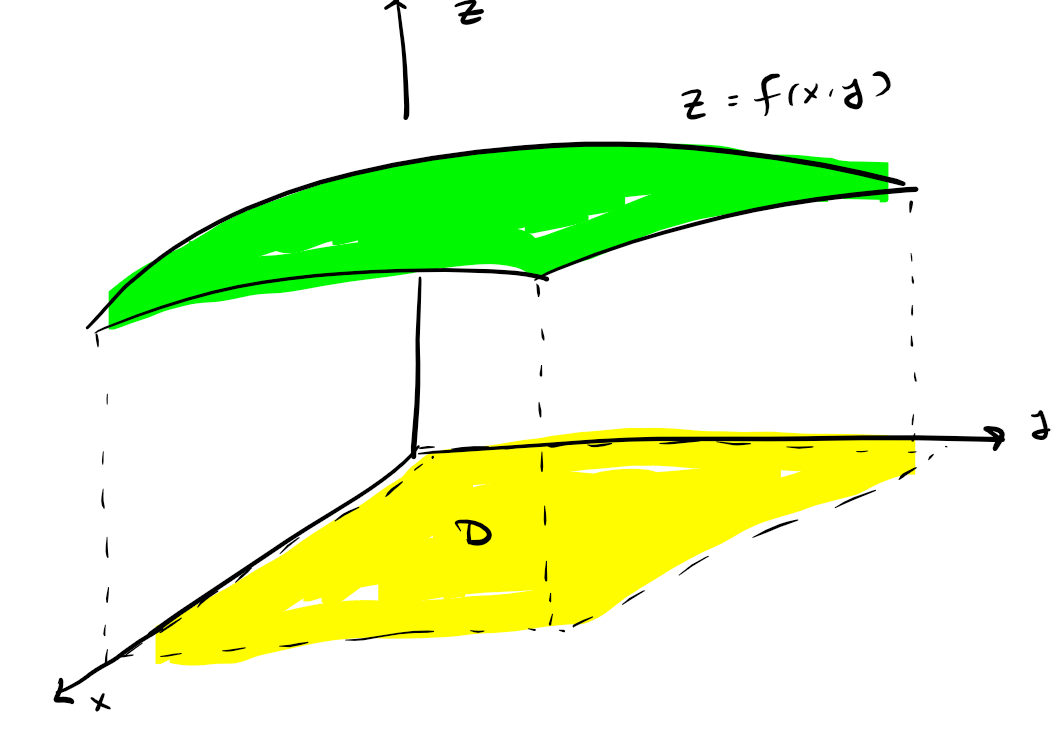
\includegraphics[width=100mm]{Images/surface-explicit}
\caption{Surface $S$ given by $z=f(x,y)$, where $f$ is a 2 variable function with domain $D$.}
\label{fig-exp-surface}
\end{figure}

In order for $S$ to be the \textit{graph} of a two variable function $f=f(x,y)$, $S$ must pass the \textbf{vertical line test}---that is, any vertical line in $\mathbf{R}^3$ may only cross $S$ at most one time.

\subsection{Level curves}
While it's somewhat possible to wrap our heads around graphs of surfaces, it's often more trouble than it's worth to try to grok the entire 3 dimensional picture. One technique is to consider what are called  \textbf{level curves} of the function. 

If you've seen a topographic map (like a hiking map with elevation lines) this is essentially the same thing: for a function $f\colon \mathbf{R}^2 \to \mathbf{R}$ we plot the \textit{implicit curves} $f(x,y)=c$ ($c$ some constant) of constant height $z$ as curves in the $xy$-plane. For instance (some of) the level curves of the saddle $f(x,y)=x^2-y^2$ can be found in Figure \ref{fig-level-curves}. (You can also play around with varying the level curve in Desmos \href{https://www.desmos.com/calculator/tazoydam1p}{as so}.)

\begin{figure}[h!]
\centering 
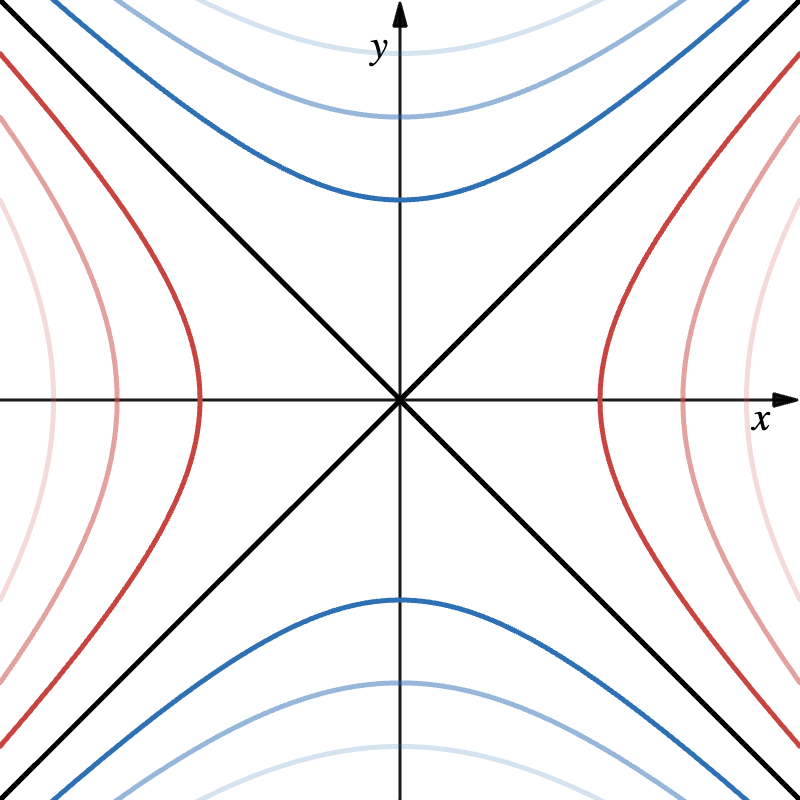
\includegraphics[height=70mm]{Images/levelcurves-saddle} 
\caption{Level curves to $f(x,y)=x^2-y^2$. Red is positive, blue is negative, black is zero. Lighter colors correspond to larger (in magnitude) outputs.}
\label{fig-level-curves}
\end{figure}


%Note that each level curve of $f$ is an implicit curve given by the equation $f(x,y)=c$ for some constant $c$. 

\subsection{Level surfaces}

If the graph of a two variable function is a surface in $\mathbf{R}^3$, what then is the graph of a three variable function? The natural answer would be that such a graph is a 3D ``thing'' that lives in $\mathbf{R}^4$, but this is not particularly easy to visualize (though it's fine mathematically). What we would like is a way to get \textit{some} information still about the behavior of such a function. 

Similar to the two variable case, given a three variable function $f=f(x,y,z)$ we can define the \textbf{level surfaces} to $f$ as the implicit surfaces $f(x,y,z)=c$ for some constant $c$. 

\subsection{Limits and continuity} 
Let's say we have a two variable function $f=f(x,y)$ and want to know whether $f$ is continuous at a point $P=(a,b)$ in its domain. What should this mean? Intuitively, this should mean that the surface given by the graph $z=f(x,y)$ has no ``rips" or "tears" in it---but how can we make this mathematical? What we need is the idea of a \textit{limit} of a two variable function. 

Let $P=(a,b)$ be given. Let's say that $C$ is a \textbf{path to $P$} if $C$ is a smooth curve parametrized by $r(t)$ such that $r(0)=P$. We then have the following

\begin{defn}[Limit of a two variable function] \label{def-limit}
	Let $f=f(x,y)$ be a two variable function and $P=(a,b)$ a point in its domain. We say that that the \textbf{limit of $f$ at $P$} equals a number $L$ if \begin{equation} \label{eq-limit-on-C} \lim_{t\to 0} f(r(t))=L\end{equation}for all parametrizations $r(t)$  of any path to $P$.
\end{defn}
Note that the term $f(r(t))$ is the restriction of $f$ to the curve $C$. This is a one variable function, so we can take the limit from \eqref{eq-limit-on-C} as the limit of a usual one-variable function. If all paths give the same limit value $L$ we write $\displaystyle \lim_{(x,y)\to P} f(x,y)$ or $\displaystyle \lim_{(x,y)\to (a,b)} f(x,y)$   for this value. 

\begin{remark}
	Definition \ref{def-limit} is the \textit{correct} definition, in that it mathematically captures our intuition from above, but it's not particularly easy to \textit{use} as a computational tool to show that a function is continuous at a point\footnote{There of course is a more mathematically rigorous definition of a limit (for instance, the $\epsilon$-$\delta$ formulation), but it gets a bit beyond the scope of our course.}. What we can do is  use this definition to show that a the limit of a function at a point does \textit{not} exist. in particular, we have the following:

\end{remark}

\begin{corr}
	If there are two distinct paths to $P$ on which $f$ has different limits, then the limit $\displaystyle \lim_{(x,y)\to P} f(x,y)$ does not exist.
\end{corr}

\begin{example}
	We should look at an example. Consider the function $f$ given by \[ f(x,y)=\dfrac{x^2-y^2}{x^2+y^2}\] Let $P=(0,0)$. Let's show that the limit of $f$ at $P$ does not exist. 
	
	Consider paths $C_1$ and $C_2$ to the origin given by $r_1(t)=(t,0)$ and $r_2(t)=(0,t)$ (these are just the straight line paths along the $x$- and $y$-axes to the origin). Then: \[ \lim_{t\to 0} f(r_1(t))=\lim_{t\to 0} \dfrac{t^2-0^2}{t^2+0^2}=\lim_{t\to 0} 1=1\] and \[ \lim_{t\to 0} f(r_2(t))=\lim_{t\to 0} \dfrac{0^2-t^2}{0^2+t^2}=\lim_{t\to 0} -1=-1\] 
	Since these values are different, the limit $\displaystyle \lim_{(x,y)\to(0,0)} f(x,y)$ does not exist\footnote{The keen-eyed student here might note that this actually does not satisfy our definition, since at the point $(0,0)$ the function $f$ is not defined. This is ``okay", there are a few fixes: one is to consider limits at points ``just outside" the domain of the function (but this gets a bit subtle). Another is to just define $f$ at the origin: for instance by saying \[ f(x,y)=\begin{cases} \dfrac{x^2-y^2}{x^2+y^2} & (x,y)\neq (0,0) \\ 0 & (x,y)=(0,0) \end{cases} \] In this case you even have a third path $C_3$ given by $r_3(t)=(0,0)$ which has limit of $f$ along $C_3$ equal to $0$. }. 
	
	
	A plot of $z=f(x,y)$ is given in Figure \ref{ex-surface-cont} (you can also see it on Desmos \href{https://www.desmos.com/3d/fhsc1uelpj}{here}).
	\begin{figure}[h!]
	\centering
	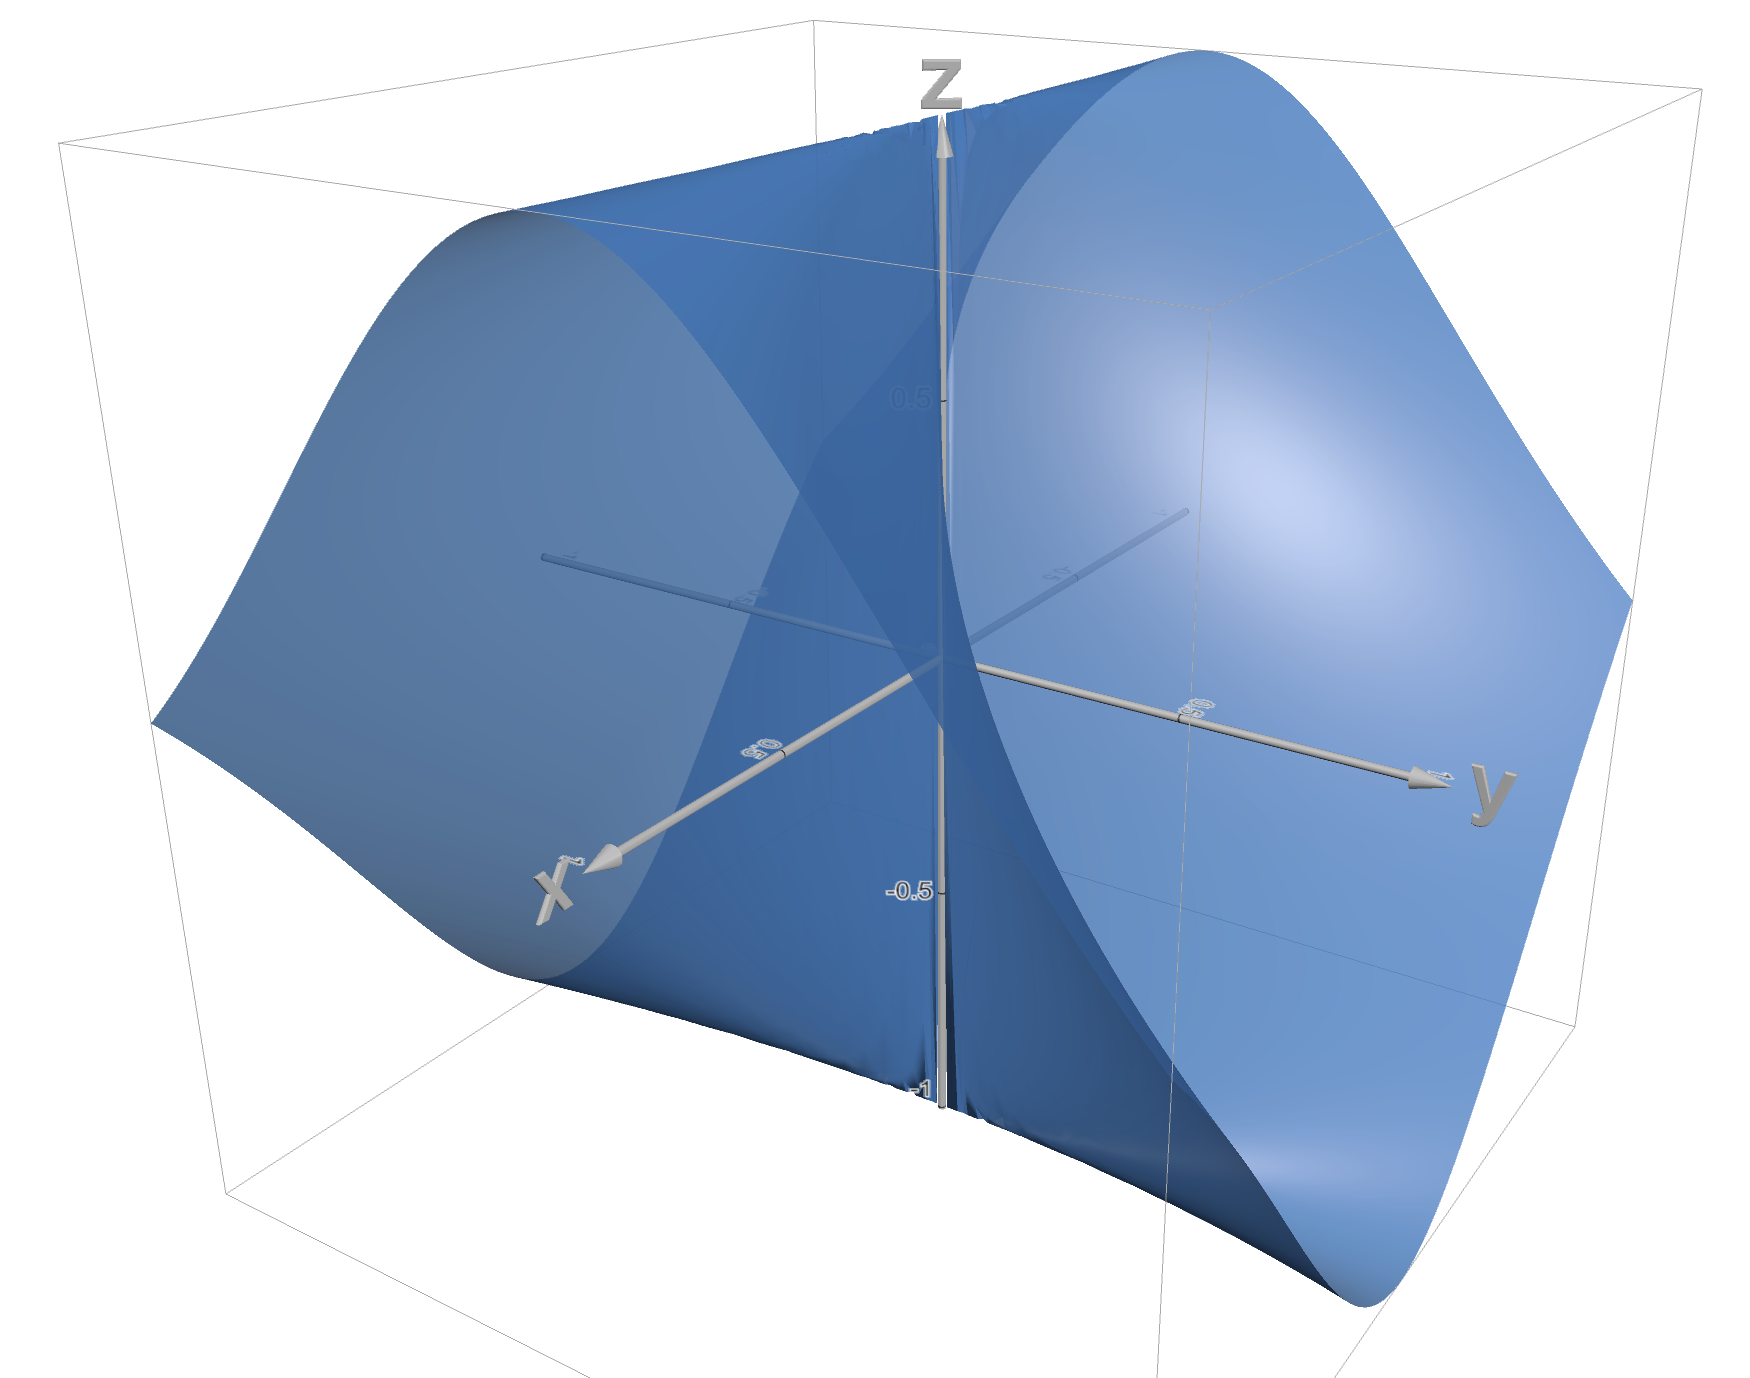
\includegraphics[width=90mm]{Images/surface-non-cont}
	\caption{Graph of $z=\dfrac{x^2-y^2}{x^2+y^2}$. Observe that the value of the function at $(0,0)$ depends on the path taken toward the origin.}
	\label{ex-surface-cont}
	\end{figure}
\end{example}


\begin{defn}[Continuity of a two variable function] \label{def-cont}
	A function $f$ is \textbf{continuous} at a point $(a,b)$ if \begin{equation} \lim_{(x,y)\to (a,b)} f(x,y) = f(a,b)\end{equation}
\end{defn}
Similarly, a function is \textbf{continuous} on a domain $D$ if it is continuous at all points in that domain. As a general rule of thumb, we'll assume that the functions we're working with are continuous unless otherwise specified. Again, demonstrating that a function actually is continuous is a lot of work, but we'll see some problems showing when a function is \textit{not} continuous at a point. 

It's also worth pointing out that the ``standard" modifications can be made to definitions \ref{def-limit} and \ref{def-cont} to talk about limits and continuity of functions of three (or more) variables. 



\subsection{Exercises} 
\begin{enumerate}[label=\arabic*.]

\item Let $f(x,y,z)=xy^2+3xz$. Find $f(1,1,1)$, and $f(0,3,2)$. Find $f(t,t^2,-t)$: what does this last expression represent?

\item Describe the domain of the following functions as regions of the $xy$-plane.
\begin{enumerate}
	\item $f(x,y)=\ln(4-x^2-y^2)$
	\item $g(x,y)=\dfrac{1}{y-x^3+1}$
\end{enumerate}

\item Sketch the graph of the following functions; describe the level curves $z=\text{const.}$ of the graph

\begin{enumerate}
	\item $f(x,y)=x+2$
	\item $g(x,y)=\sqrt{4-x^2-y^2}$
	\item $h(x,y)=x^2-y^2$
	\item $C(x,y)=\sqrt{x^2+y^2}$
\end{enumerate}

\item Let $f(x,y,z)=x^2+(y-1)^2+z^2$. Describe the level surfaces of $f$. Give the equation of the level surface of $f$ passing through the point $(1,-2,1)$

\item \textit{Conic sections}. Show that $z^2=x^2+y^2$ gives the graph of a (two-sided) cone. Describe the cross sections of this cone for $z=k$, $k$ a constant. Do the same for $x=k$, and $y=k$ $k$ a constant. 

\item The following are some (untagged) level curves of a function $f\colon \mathbf{R}^2\to \mathbf{R}$. Determine a surface which could have such level curves.
\[ \text{a}. 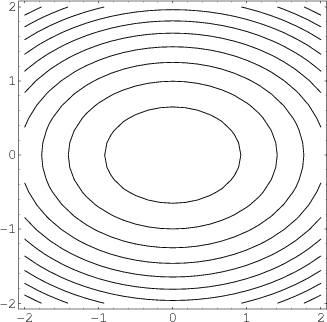
\includegraphics[height=50mm]{Images/ws7-lc2} \qquad 
	 \text{b}. 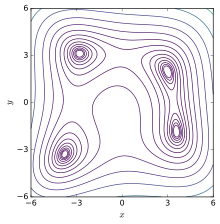
\includegraphics[height=60mm]{Images/ws7-lc3} %update these
	 \]


\item \textit{True or false}? If every level curve of a function $f(x,y)$ is a line, then the graph $z=f(x,y)$ is a plane. 

\item Imagine a cube-shaped room has temperature function $T=T(x,y,z)$. Suppose the room is empty except for one (very hot) candle burning in the middle of the room. Can you determine what the level surfaces of constant temperature should be? What if instead of a candle the floor of the room was (uniformly distributed) lava? 

\item Consider the path to the origin along the straight line of slope $m$ (i.e., line $y=mx$). Show that \[ \lim_{(x,y)\to(0,0) }\dfrac{xy}{x^2+y^2}\] evaluated on such paths to the origin depends on $m$, and therefore does not exist.

\item It's tempting to think that if $\lim_{(x,y)\to P}f(x,y)$ exists and is equal when evaluated on any \textit{straight line paths} to $P$ that $\lim_{(x,y)\to P}f(x,y)$ should exist. This is unfortunately not true. In this problem we'll see why. 

Let $f(x,y)=\dfrac{x^2y}{x^4+y^2}$. 
\begin{enumerate}
	\item Show that $\displaystyle \lim_{(x,y)\to (0,0)}f(x,y)=0$ along all straight line paths $y=mx$ to the origin. 
	\item Consider parabola paths $y=mx^2$ to the origin. Show that on such paths, the limit of $f$ depends on $m$, and therefore does not exist
\end{enumerate}

\item Does $\displaystyle \lim_{(x,y)\to (0,0)} \dfrac{\sin(x^2+y^2)}{x^2+y^2}$ exist? Explain your answer.
\end{enumerate}



Suggested additional exercises: \textit{Stewart} Section 14.1


\section{Partial derivatives and the gradient}

Finally we get to differential calculus of multivariable functions. The first observation is that the notion of \textit{the} derivative of a multivariable function $f$ is not entirely well-defined. We'll see that the \textit{gradient} is the thing that could most reasonably be called \textit{the} derivative, but it's not the same type of thing as $f$ (more on this soon). What we have instead are \textit{partial} derivatives---i.e., derivatives taken with respect to one of the (many) variables of a multivariable function. 


\begin{defn}[Partial derivative] Let $f=f(x,y)$ be a function of two variables. The \textbf{partial derivatives} $f_x$ and $f_y$ of $f$ are calculated at a point $(a,b)$ via the limits:

\begin{equation} 
	f_x(a,b)=\lim_{h\to 0} \dfrac{f(a+h,b)-f(a,b)}{h} \qquad \qquad f_y(a,b)=\lim_{h\to 0} \dfrac{f(a, b+h)-f(a,b)}{h} \label{partials}
\end{equation}
\end{defn}

with the ``obvious'' modifications made for a function of three (or more) variables. Now, just like with one-variable calc, we almost never use these limits to calculate the derivatives, instead we can just the derivative rules (like product rule, quotient rule, etc.), treating the other variables as constants. For instance, the $x$ partial, $f_x$, is computed by treating all instances of the variable $y$ (or other variables) as constants, differentiating only with respect to $x$.

\begin{remark}[Notation] For the $x$ partial of a function $f=f(x,y)$ we use the following notation \begin{equation} f_x= \dfrac{\partial}{\partial x} f=D_x f\end{equation} ditto with the $y$ partials ($z$ partials, etc. if $f$ has more than two variables). The first two are the most common, but the last can be useful as well. The symbol $\partial$ is called \textbf{partial} (or sometimes ``curly d'', taking inspiration from the $d/dx$ notation from one-variable calc.). \end{remark}

\subsection{Higher order derivatives} Since the partial derivatives of a multivariable function are again multivariable functions, we can take more derivatives (as long as the corresponding limits exist). Second and higher order derivatives are calculated as \begin{equation} (f_x)_y=f_{xy},\qquad \dfrac{\partial }{\partial y} \left(\dfrac{\partial }{\partial x}f\right)=\dfrac{\partial^2 }{\partial y \partial x}f, \qquad D_y \left(D_x f\right)=D_{yx}f, \quad \text{etc.}\end{equation}


for these various notations. Note the order in which the ``take derivative" operation is applied. Actually, in most cases, this is not really something we need to be concerned with writing down precisely, due to the following theorem.

\begin{thm}[Clairut's theorem]  \label{Clairut-thm} If $f=f(x,y)$ is a function such that all of the second order partial derivatives $f_{xx}, f_{yy}, f_{xy}$ and $f_{yx}$ exist and are continuous, then $f_{xy}=f_{yx}$.
\end{thm}

Clairut's theorem applies really to any mixed partials of a multivariable function, in essence telling us that the ``order of differentiation'' does not matter, just the total number of each partial derivative variable. Like most theorems, there are some conditions needed for this to apply, but almost any function we actually write down (in this class, at least) will meet the necessary conditions, so we will make frequent use of this theorem without necessarily checking the conditions.


\subsection{The gradient}

While the partial derivatives independently may not tell us the whole story about the rate of change of a multivariable function, the collection of first-order partial derivatives has \textit{all} of the information about how that function changes. 

\begin{defn}[Gradient] Suppose $f$ is a function of two or three variables (either $x,y$ or $x,y,z$) such that all first-order partial derivatives of $f$ exist. The \textbf{gradient} of $f$, written $\nabla f$, is the \textit{vector} given by \begin{align}  \label{del}
	&\nabla f =(f_x,f_y) & \hspace{10mm} & (\text{if $f$ is a function of two variables})  \nonumber \\
	&\nabla f =(f_x,f_y,f_z) & & (\text{if $f$ is a function of three variables}) 
\end{align}
\end{defn}

\begin{remark}Note that the gradient of a scalar function $f$ is a vector-valued function, whose number of output components is the same as the number of input components of $f$ (this is called a vector field, as we'll see in Section \ref{sec-vector-field}). There's nothing special about two or three variables as written in \eqref{del}, and you can probably guess what the gradient of a function of $n$ variables should be. The symbol $\nabla$ is often referred to as either the ``gradient operator'' or, more shortly, ``del''\footnote{You might also see people call it ``nabla''---the symbol evidently predates the word. The word \textit{nabla} comes from the Greek $\upnu \upalpha \upbeta \uplambda \upalpha$ which roughly means ``harp'' in modern English (note the shape of a harp bears resemblance to the symbol $\nabla$).}.\end{remark}

What's remarkable about the gradient? The following theorem tells us its main properties. 

\begin{thm}[Gradient points in direction of max increase] \label{gradient-properties} For a scalar function $f$ and point $P$ in the domain of $f$, the vector $\nabla f(P)$ has the following features:
\begin{itemize}
\item $\nabla f(P)$ points in the direction of greatest increase of the function $f$ (as a vector in the domain of $f$, originating at point $P$)
\item $| \nabla f (P) |$ is the \textit{maximum rate of change} of $f$ at point $P$. 
\end{itemize}
\end{thm}

Said differently, if you are on a mountain, the gradient is like a compass which points you towards the direction of steepest ascent and constantly updates as you change your direction. You may wonder how this is possible, this is what we'll cover next. 

\subsection{The directional derivative}

Given a multivariable function $f$, the partial derivatives $f_x,f_y$, etc. tell us about the rate of change in the directions corresponding to the coordinate axes in the domain of $f$. But what about other directions? Say we have a unit\footnote{That $u$ be a unit vector here is important: there are a bunch of vectors that point in any given direction, the unit vector is the one which ``ignores the length".} vector $\vec{u}$ and a point $P$ in the domain of $f$. The \textbf{directional derivative} of $f$ at point $P$ in the $\vec{u}$ direction is given by \begin{equation} D_{\vec{u}} f(P)= \lim_{h\to 0^+} \dfrac{f(P+h \vec{u})-f(P)}{h} \end{equation} (That hat here on the $\vec{u}$ vector is mostly just to emphasize that it is a direction, we'll typically drop it). This limit is possible to calculate, but if this quantity is desired it's much easier to use the formula provided by the following theorem:

\begin{thm} Let $f$ be a multivariable function such that $\nabla f$ is defined and $u$ be a unit vector (of the same number of components that $f$ has inputs). Then {directional derivative} of $f$ at a point $P$ in the direction of $u$ is given by \begin{equation} \label{dirder} 
	D_u f(P)=\nabla f (P) \cdot u
\end{equation}
\end{thm}
For instance, if $f=f(x,y)$ is a function of two variables, $P=(a,b)$, and $u=(u_1,u_2)$; equation \eqref{dirder} becomes: \[ D_u f(a,b) = \nabla f(a,b) \cdot u= (f_x (a,b), f_y(a,b)) \cdot (u_1,u_2)\]

\begin{proof}
This is actually fairly straightforward to show. Let $f=f(x,y)$ be given, $u=(u_1,u_2)$ a unit vector, and $(a,b)$ a point in the domain of $f$. Then \begin{align*} D_u f(a,b)&=\lim_{h\to0^+} \dfrac{f(a+u_1 h, b+u_2 h)- f(a,b)}{h} \\ 
&= \lim_{h\to 0^+} \dfrac{ f(a+u_1 h, b+u_2 h)- f(a, b+u_2 h) + f(a,b+u_2 h) - f(a,b)}{h} \\
&=\lim_{h\to 0^+} \dfrac{ f(a+u_1 h, b+u_2 h)- f(a, b+u_2 h)}{h} +  \dfrac{ f(a, b+u_2 h)- f(a, b)}{h} \\
&=\lim_{h\to 0^+} \left( \dfrac{ f(a+u_1 h, b+u_2 h)- f(a, b+u_2 h)}{u_1 h}\right) u_1 +  \left( \dfrac{ f(a, b+u_2 h)- f(a, b)}{u_2 h}\right) u_2 \\
&=f_x(a,b) u_1+f_y(a,b) u_2 \\
&= \nabla f (a,b) \cdot u\end{align*} 
The same idea can be modified for functions of three or more variables\footnote{There is a very slight problem here if one of the components of $u$ happens to be zero, but I leave it to you to figure out how to avoid this}.
\end{proof}


%It's possible (but a bit tedious) to show where formula \eqref{dirder} comes from by the limit definition of the derivative. An alternate explanation will be given as an exercise using the multivariable chain rule in section \ref{ch-rule-ex}.

\begin{remark}
	It's worth pointing out that the main properties of the gradient from theorem \ref{gradient-properties} are entirely derived from equation \eqref{dirder}. Recall that the dot product tells us about the angle between vectors. Let a multivariable function $f$ and unit vector $u$ be given, and let $\theta$ be the angle between $u$ and $\nabla f$. Then \begin{equation} |D_u f| = |\nabla f| |u| \cos \theta=|\nabla f | \cos \theta\end{equation}
	This tells us a few things: \begin{itemize}
		\item $D_u f$ is greatest when the angle between $u$ and $\nabla f$ is $0$---that is, $u$ and $\nabla f$ point in the same direction and $D_u f=|\nabla f|$
		\item $D_u f$ is the \textit{most negative} when $\theta=\pi$, which is to say that $u$ and $\nabla f$ point in the opposite direction and $D_uf=-|\nabla f|$
		\item $D_u f=0$ whenever $u$ and $\nabla f$ are perpendicular. Note that $D_u f=0$ means that the direction $u$ must be tangent to the level set (i.e., level curve, level surface, etc.) of the function $f$. In other words, $\nabla f$ is perpendicular to any level set of $f$. 
	\end{itemize}

\end{remark}





\subsection{Exercises}
\begin{enumerate}[label=\arabic*.]
\item Compute $f_x$ and $f_y$ for the following functions

\begin{enumerate}
	\item $f(x,y)=2x+y$
	\item $f(x,y)=e^{xy}(y-x)$
	\item $f(x,y)=\ln(x\cos(y))$
	\item $f(x,y)=\tan(xy^2+1)$
\end{enumerate}


\item Show that $f_{xy}=f_{yx}$ for the following functions

\begin{enumerate}
	\item $f(x,y)=8x^2y+5xy^3-2x$
	\item $f(x,y)=e^{x}\sin(y)$
	\item $f(x,y)=\dfrac{x+y}{x^2-3y}$
\end{enumerate}

\item The \textit{Cauchy-Riemann equations} are an important system of equations of partial derivatives of functions used in complex analysis. Given $u(x,y)$ and $v(x,y)$, we say $u,v$ satisfy the Cauchy-Riemann equations if 
\begin{equation} \dfrac{\partial u}{\partial x}=\dfrac{\partial v}{\partial y} \text{ and } \dfrac{\partial u}{\partial y}=-\dfrac{\partial v}{\partial x}\end{equation}

Show that $u(x,y)=x^2-y^2$ and $v(x,y)=2xy$ satisfy the Cauchy-Riemann equations. 

%\item A heat function $z(x,t)$ tells the temperature of a 1-dimensional object in terms of time $t$ satisfies the partial differential equation $z_t=z_{xx}$ (this is a form of the \textit{heat equation}.)   Show that $z=e^{-t}\sin(x)$ satisfies the heat equation. 




\item Compute the directional derivative $D_{u} f$ of the given function $f$ at the indicated point.

\begin{enumerate}
	\item $f(x,y)=\cos(2x+3y)$, $P=(3,-2)$, $u=(3/5,4/5)$
	\item $f(x,y)=e^{xy^2}$, $P=(0,1)$, $u=(-1/2,\sqrt{3}/2)$
	\item $f(x,y,z)=\ln(xz+y)$, $P=(1,0,\pi)$, $u=(1/\sqrt{2}, 1/\sqrt{2},0)$
\end{enumerate}

\item Determine the directional derivative of $f(x,y)=\sqrt{xy}$ at a generic point $(x,y)$ in the direction of the vector $u=(1,2)$. (\textit{Hint: first turn $u$ into a unit vector}.)

\item For each of the following functions $f$, compute the gradient $\nabla f$. Use the gradient to find the direction of max increase for each of the functions at the point $P=(1,1)$ (for a,b) or $P=(1,1,-1)$ for c.

\begin{enumerate}
	\item $f(x,y)=5x^2+y^6$
	\item $f(x,y)=(x^2+y^2)^{3/2}$
	\item $f(x,y,z)=y^2z e^x$
\end{enumerate}

\item Given that $f(x,y)=3x^2-y^2$ find all points $(x,y)$ with $|\nabla f|=6$. 


\item \textit{True or false}. Determine if each of the following statements is true or false. Give a brief justification of your answer.

\begin{enumerate}
	\item If $z=f(x,y)$ is the graph of a plane, then $f_x$ and $f_y$ are constants. 
	\item If the level curves of $f(x,y)$ are horizontal lines in the $xy$-plane, then $f_{x}=0$.
	\item If $f(x,y)=x^2y^3$ then $f_{xyx}=f_{yxx}$
	\item If there is a unit vector $u$ such that $D_u f(x,y)=0$ for all points $(x,y)$ then $f$ is a constant function
	\item If $f$ is a function and $(a,b)$ some point with $f_x(a,b)=f_y(a,b)=0$, then $D_uf(a,b)=0$ for all unit vectors $u$.
	\item The gradient of a function $f$ evaluated at a point $P$ is always perpendicular to the level curve of $f$ passing through $P$.
	\item If $y=x^2$ is a level curve of $f$, then $f_x(0,0)=0$. 
\end{enumerate}
\end{enumerate}

Suggested additional exercises: \textit{Stewart} sections 14.3, 14.6

%%%
\section{Tangent planes and differentials} \label{sec-tan-plane}

While the theory of Taylor series extends nicely to multivariable functions, we wont be venturing farther than just the first-order linear approximation to a two variable function. Recall that for a one variable function $f=f(x)$ that the \textit{linear approximation} to $f$ at $x=a$ is the tangent line \begin{equation} L_a(x)=f(a)+f'(a)(x-a)\end{equation} Idea being, that for $x$ near $a$ that $L_a(x)\approx f(x)$. In the case a two-variable function, the correct analogue for this line is the \textit{tangent plane}.

\begin{example}[Tangent line from the gradient]
To motivate the upcoming construction of the tangent plane, let's consider the following construction of the tangent line. Let $C$ be some curve in $\mathbf{R}^2$ given by the implicit function $F(x,y)=0$. Suppose that $P=(a,b)$ is a point on $C$. We want to create the tangent line to $C$ at $P$. Note that $\nabla F(a,b)$ is a vector which is perpendicular to $C$ by construction. Therefore, any point $(x,y)$ on the desired tangent line must satisfy (see Figure \ref{fig-tan-line}) \[\nabla F(a,b) \cdot (x-a,y-b)=0.\]
\begin{figure}[h!]
\centering
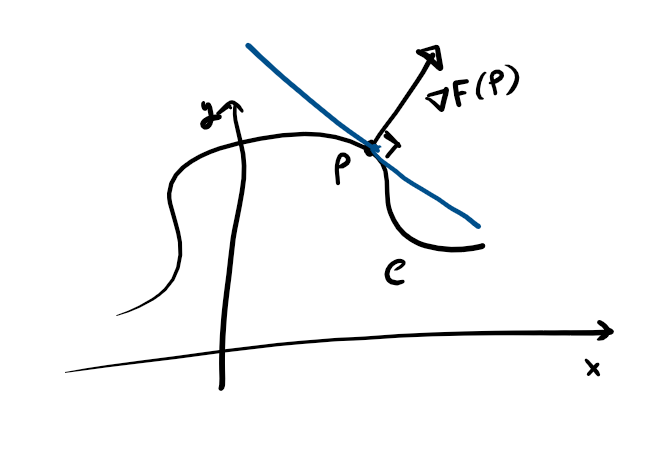
\includegraphics[width=70mm]{Images/tangent-line-grad}
\caption{Tangent line to an implicit curve $F(x,y)=0$ at point $P$}
\label{fig-tan-line}
\end{figure}
In the case that $C$ is described by the \textit{explicit} function $y=f(x)$, we can write $F(x,y)=y-f(x)$. Then $\nabla F=(-f',1)$ and so the above equation becomes \[ (-f'(a),1)\cdot(x-a,y-b)=0\] This may look somewhat strange, but actually this is just point-slope form: rearranging, expanding the dot product we get $-f(a)(x-a)+y-b=0$. Since $b=f(a)$, we therefore have \[y=f(a)+f'(a)(x-a).\]

\end{example}

\subsection{Tangent plane}
The following definition of the tangent plane to a surface is motivated by the previous example. 

\begin{defn} Let $S$ be a surface in $\mathbf{R}^3$ given by the implicit function $F(x,y,z)=0$ and $P=(a,b,c)$ a point on $S$. Repeating the idea from the previous example, we have that $\nabla F(a,b,c)$ must be perpendicular to this surface, and therefore the tangent plane is given by the equation\footnote{Recall the plane builder equation \eqref{plane-creator}} \begin{equation} \label{tp-1}
	\nabla F(a,b,c) \cdot (x-a,y-b,z-c)=0
\end{equation}
\end{defn}

\begin{figure}[h!]
\centering
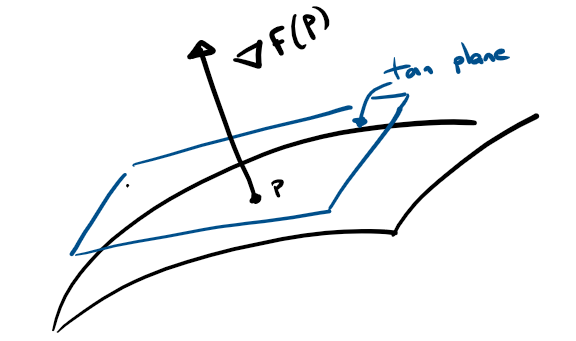
\includegraphics[width=80mm]{Images/tan-plan-grad}
\caption{Tangent plane to an implicit surface $F(x,y,z)=0$ at point $P$}
\label{fig-tan-plane-grad}
\end{figure}

\begin{remark}Note if we have an \textit{explicit surface} $S$ given by an equation $z=f(x,y)$, then set $F$ to be the function \[F(x,y,z)=z-f(x,y)\] and observe that $S$ is now given by the implicit function $F(x,y,z)=0$. We can then calculate that $\nabla F=(-f_x, -f_y, 1)$.  Therefore if $P=(a,b,c)$ is a point on $S$, then $c=f(a,b)$ then \eqref{tp-1} becomes \[ (-f_x(a,b),-f_y(a,b),1)\cdot (x-a, y-b,z-f(a,b))=0\] Combining all this we get the following: \end{remark}

\begin{corr} If $f=f(x,y)$ is a differentiable function of two variables and $(a,b)$ a point in the domain of $f$, then the \textbf{tangent plane} to $f$ at $(a,b)$ is the plane given by $z=P_{(a,b)}(x,y)$ where the function $P_{(a,b)}$ is given by \begin{equation} \label{tp-2} P_{(a,b)}(x,y)=f(a,b)+f_x(a,b)(x-a)+f_y(a,b)(y-b)\end{equation}
\end{corr}

Similarly, if $(x,y)$ is a point \textit{near} $(a,b)$, then $P_{(a,b)}(x,y)\approx f(x,y)$. Said differently, the tangent plane is the best plane-approximation to $f$ near $(a,b)$

\subsection{Differentials}
A similar idea to the tangent plane is the \textit{differential}. The exact definition of what a differential is is a bit beyond the scope of our class\footnote{But please feel free to ask me about if you're interested} but for our purposes the following will suffice.

\begin{defn}[The differential] Let $f=f(x,y)$ be a two variable function. The \textbf{differential} of $f$ is the following expression \begin{equation} \label{diff} df=f_x \,dx+f_y \,dy \end{equation}
\end{defn}

\begin{remark}On its own this doesn't look like much, or even really tell us what to do with it. Our use will be the following: given a point $(a,b)$ and small displacement vector $(d x, d y)$, $df$ is evaluated as \[f_x(a,b)\, d x+f_y(a,b) \, d y.\] This expression is really just the tangent plane without the constant term $f(a,b)$, but its inputs should be thought of as vectors from $(a,b)$ rather than points in the domain of $f$. Differentials for us compute the \textit{approximate change} of a function when moving its input from a ``known'' value $(a,b)$ to a nearby (and presumably more difficult to calculate) value $(a+d x, b+d y)$\footnote{Really what's happening here is the differential of $f$ is a \textit{linear transformation} on defined on the tangent plane of the domain of $f$. This level of subtlety is not needed for this term. }. 
\end{remark}

As with the other topics, these ideas can be readily transferred to functions with three or more variables. The only difference being that ``plane'' gets replaced by ``hyperplane''---the appropriate $n$-dimensional linear ``thing''---and the functions and equations take on more terms.

\subsection{Exercises}

\begin{enumerate}[label=\arabic*.]

\item Compute the following differentials, leave your answer in terms of $dx$ and $dy$.
\begin{enumerate}
	\item $z=e^{xy}\cos(x)$
	\item $w=x^3y^2+z^2+yz^2$
	\item $w=\cos(xy)+\sqrt{yz}$
	\item $w=\arctan(xyz)$
\end{enumerate}

\item Give the equation for the tangent plane to $f$ at the indicated point $(a,b)$
\begin{enumerate}
	\item $f(x,y)=xy^2+\tan(x)$; $(0,1)$
	\item $f(x,y)=\ln(xe^y-1)$; $(2,0)$
\end{enumerate}

\item Use the differential to approximate the change in the $f(x,y)=\dfrac{xy}{x+y}$ between points $(1,1)$ and $(1.02,0.99)$. Do the same for $g(x,y,z)=\cos(xy+\pi z)$ from $(0,1,1)$ to $(0.1,1.1,0.9)$.

\item Let $\alpha,\beta$ be real numbers. Show that the linear approximation to $f(x,y)=x^{\alpha}y^{\beta}$ at $(1,1)$ is given by $L(x,y)=1+\alpha(x-1)+\beta(y-1)$.

\item The \textit{ideal gas law} states that pressure $P$, temperature $T$, and volume $V$ of a contained gas are related by \[ P= \dfrac{kT}{V}\] for some constant $k$. Approximate the total error of $P$ if the measured temperature has a maximum error of $2\%$ and volume has a maximum error of $4\%$.

%\item In this problem we'll show where the equation for the tangent plane \eqref{tp} comes from using the gradient. Let $f=f(x,y)$ be a two variable function and $(a,b)$ some point in the domain. Define a function $F$ by \[F(x,y,z)=z-f(x,y)\]

%\begin{enumerate}
%	\item Explain why the surface produced by the graph $z=f(x,y)$ is the level surface $F(x,y,z)=0$.
%	\item The vector $\nabla F$ is then perpendicular to this surface. Compute $\nabla F(a,b,f(a,b))$ (\textit{this will be in terms of $a,b$})
%	\item Show that \eqref{tp} comes from the plane builder equation (see \eqref{plane-creator}) \begin{equation}\nabla F(a,b,f(a,b)) \cdot (x-a, y-b,z-f(a,b))=0\end{equation}

%\end{enumerate}

\item The total resistance $R$ of two resistors of resistance $R_1$ and $R_2$ connected in parallel is given by \[ \dfrac{1}{R}=\dfrac{1}{R_1}+\dfrac{1}{R_2}.\] Suppose two 49.9$\Omega$ resistors are connected in parallel. Compute the approximate change in resistance if one of the resistors is replaced with a more standard 47$\Omega$ resistor. 
\end{enumerate}



Suggested additional exercises: \textit{Stewart} Section 14.4 


\section{The chain rule}

In ordinary one variable differential calc, the \textit{chain rule} is a technique for differentiating a composite of two or more functions in terms of its parts. That is, if $f=f(x)$ but $x=x(t)$ is a function of $t$, then we can calculate \begin{equation} \dfrac{d}{dt} f(x(t))= \dfrac{df}{dx} \dfrac{dx}{dt}\end{equation}

With multivariable functions the idea is essentially the same: the simplest form of the chain rule would apply when, say, $f=f(x,y)$ is a function of $x,y$ but $x=x(t)$ and $y=y(t)$ are separately functions of a third variable $t$ (think of $f(x(t),y(t))$ then as asking about $f$ \textit{along} the parametric curve $(x(t),y(t))$.) Though you \textit{could} just evaluate \[\dfrac{d}{dt} \lbrack f(x(t),y(t)\rbrack\] by first evaluating the composite, the \textit{chain rule} tells us how this derivative breaks down into the constituent partial (and ordinary) derivatives. 

\subsection{Multivariable chain rule, main formulation} Let $f$ be a two variable function and $r(t)=(x(t),y(t))$ a smooth curve within the domain of $f$. With this set up, the \textbf{multivariable chain rule} is the following statement: 
\begin{equation} \dfrac{d}{dt} f(x(t),y(t))=f_x \dfrac{dx}{dt} + f_y \dfrac{dy}{dt} \label{cr-1}\end{equation}
Using a similar interpretation from the differential and directional derivative, it's often conceptually useful to interpret \eqref{cr-1} using the gradient as: \[ \dfrac{d}{dt} f(x(t),y(t)) = \nabla f(x(t),y(t)) \cdot (x'(t), y'(t)) \] So, if $f(x(t),y(t))$ is the function restricted to the curve $r(t)=(x(t),y(t))$ then $\dfrac{d}{dt} f$ comes from two pieces of information: (i) the gradient $\nabla f$ at a point along the curve, (ii) the tangent vector to the curve.


\subsection{Change of variable chain rule} There are other forms of the chain rule. For instance, we'll be interested in \textit{change of variable} transformations $x=x(u,v)$ and $y=y(u,v)$ in how they relate to multivariable functions. In this instance, if $f=f(x,y)$ then the chain rule would tells us:
\begin{equation} \label{cr-2} f_u = f_x x_u+f_y y_u \qquad \qquad f_v = f_x x_v+f_y y_v\end{equation} 


\subsection{Other chain rules} All of these chain rules essentially amount to the same process: take all the partials of the outer function, multiply each by the partial (or ordinary) derivative of the inner with respect to whatever variable you are attempting to differentiate with, then add up all of these terms. Said differentially, it's always the gradient of the outer function \textit{dotted} with the tangent vector of the inner in the direction of the variable you are differentiating with respect to (for \eqref{cr-2} this will make more sense when we get to parametrized surfaces).

\subsection{The implicit function theorem}
There's one theorem here, but it's a bit clunky to state in full generality. Here it is in its simplest form.

\begin{thm}[Implicit function theorem] Let $C$ be the curve in the $xy$-plane given by the implicit function $F(x,y)=0$ (assume that $F_x,F_y$ exist and are continuous). Then, for any point on this curve with $F_y\neq 0$, \begin{equation} \dfrac{dy}{dx}= -\dfrac{F_x}{F_y}\label{ift}\end{equation}
\end{thm}
\begin{proof}
	This is actually not too difficult to show: apply $\partial/\partial x$ to both sides of the equation $F(x,y)=0$ to get \begin{align*}
		\dfrac{\partial}{\partial x} F(x,y)&= \dfrac{\partial}{\partial x} 0 \\
		F_x(x,y)+F_y(x,y)\dfrac{dy}{dx}&=0\\
		\dfrac{dy}{dx}&=\dfrac{-F_x(x,y)}{F_y(x,y)}
	\end{align*}
\end{proof}
That is to say, the slope of the tangent line to the curve can be computed by the partial derivatives of its defining implicit function\footnote{You may recall \textit{implicit differentiation} from calculus 1. This allows you to avoid doing the somewhat laborious process of finding $dy/dx$ for such implicit curves}. 


\begin{remark}[Implicit function theorem for implicit surfaces] The full theorem is actually quite a bit more general\footnote{It involves implicit functions defined by \textit{systems} of equations} and somewhat tedious to write out. There is a nice extension to functions of three variables---namely, if $S$ is a surface defined by the implicit function $F(x,y,z)=0$, then at any ``reasonable'' point on the surface one of the variables, say $z$, can be treated as a function of the other two. Then, the partial derivatives of this function are computed as follows (note the rule: it's the negative reciprocal of ratios of partials).  \[ \dfrac{\partial z}{\partial x}=-\dfrac{F_x}{F_z}, \qquad \dfrac{\partial z}{\partial y} = -\dfrac{F_y}{F_z} \]
\end{remark} 
\subsection{Exercises} \label{ch-rule-ex}
\begin{enumerate}[label=\arabic*.]

\item Given the following functions for $z=z(x,y)$ and $x=x(u,v), y=y(u,v)$, compute $\partial z/\partial u$ and $\partial z/\partial v$ at the indicated point via the chain rule. 

\begin{enumerate}
	\item $z=x^2y-\tan (xy)$, \quad $x=u^2+2v, y=3\sin v$; \quad $(u,v)=(0,\pi/6)$
	\item $z=\cos (y\sin x)$, \quad $x=2uv, y=u^2-e^{v}$; \quad $(u,v)=(0,0)$
	\item $z=\ln(2+x)+y$,\quad $x=u-v, y=\arcsin(v-u)$\quad $(u,v)=(1/2,0)$
\end{enumerate}

\item Consider the \textit{polar substitution} $x=r\cos \theta$, $y=r\sin \theta$. Let $T=x^2y-y^3+10x$. Compute $T_r$ and $T_{\theta}$. Do the same for $T=e^{xy}-e^{x+y}$

\item Later in this course (see section \ref{spherical-coord}) we'll learn about \textit{spherical coordinates}. Use the following functions \[x=\rho \sin \varphi \cos \theta, \quad y=\rho \sin \varphi \sin \theta, \quad z=\rho \cos \varphi\] to find $\partial w/\partial \varphi$ and $\partial w/\partial \theta$ for $w=4x^2-y^2+z^4-2$.


\item An equation of the form $f(x,y)=0$ describes some of curve in the $xy$-plane. Use implicit differentiation to derive the \textit{implicit function theorem} from \eqref{ift}.

\begin{enumerate}
\item Use the implicit function theorem to compute $dy/dx$ for the curve given by $x^2y-ye^{x}+y=0$. 
\item Show that $(0,1)$ lies on the curve from part a. and find the tangent line at that point.%change this stupid problem
\end{enumerate}

\item Let $f=f(t)$ be a differentiable function and set $z=f(x^2-y^2)$. Show that $y z_x+xz_y=0$.

\item The \textit{wave equation} is a differential equation which states \[ u_{tt}=c^2 u_{xx}\] where $u(x,t)$ is the displacement as a function of position $x$ and time $t$, and $c$ is some constant. 
\begin{enumerate}

\item Show that any function of the form $u(x,t)=f(x+ct)$ (where $f$ is a twice differentiable function) satisfies the wave equation $u_{tt}=c^2 u_{xx}$
\item Show that $\sin(x+2t)$ and $\cos(x+2t)$ are solutions to the wave equation $u_{tt}=4u_{xx}$
	
\end{enumerate}

\item \textit{Second derivative formulas}

\begin{enumerate}

\item Let $z=z(x,y)$, $x=x(t)$ and $y=y(t)$. Determine a formula for $\partial^2 z/\partial t^2$ in terms of the derivatives of $x$ and $y$ and the partial derivatives of $z$. 

\item Like in problem 4, a curve is defined implicitly by $f(x,y)=0$. Show the following: \begin{equation} \dfrac{d^2y}{dx^2}=\dfrac{ f_{xx} f_y^2-2f_{xy}f_xf_y+f_{yy}f_{x}^2}{f_y^3}\end{equation}

\end{enumerate}

\item In this problem, we'll give another explanation for  why equation \eqref{dirder} is the correct expression for the directional derivative of $f$. Let $f$ be given, $P$ a point in the domain of $f$, and $u$ be a unit vector. Let $r(t)$ be a parametric curve such that $r(0)=P$ and $r'(0)=u$ (why does such a curve exist?). 

Use the multivariable chain rule to explain the following calculation \[ D_uf(P)=\left. \dfrac{d}{dt} f(r(t)) \right|_{t=0} = \nabla f(P)  \cdot r'(0)=\nabla f(P)\cdot u \]
\end{enumerate}

Suggested additional exercises: Section 14.5 





%%%
\section{Extrema of two variable functions}

An \textbf{extremum} (plural \textbf{extrema}) is a point in the domain of a function $f$ where that function is either largest or smallest. Finding extrema is an extremely useful application of calculus (you may recall this from one-variable optimization problems in calc 1). We'll cover two similar but distinct type of extrema problems. First \textit{local} extrema, then second \textit{global} extrema. 

\subsection{Local extrema}
Local extrema can be thought of as the largest/smallest values of the function ``nearby'' the given point. In one-variable calculus you may recall the following. Any \textit{local} extremum of a (differentiable) function $f$ must occur at a value $x$ such that $f'(x)=0$ (or $f'(x)$ does not exist). In nice cases, we can use the second derivative to test for concavity at a critical point, and determine local information about whether a given critical point is a max or a min.

\begin{defn}[Critical point] A point $(a,b)$ in the domain of $f$ is called a \textbf{critical point} if both $f_x(a,b)=0$ and $f_y(a,b)=0$. 
\end{defn}

Note that this is the same as $\nabla f(a,b)=(0,0)$ (in terms of what the gradient tells us, it's useful to think of the zero vector as the gradient ``breaking down'' at a point and not being able to give us a direction of greatest change\footnote{For instance, at the bottom of the parabola $f(x,y)=x^2+y^2$ \textit{all} directions are directions of increase of the same amount, the only thing the gradient can return so that $\nabla f$ is a differentiable function is the zero vector}.) 

As in one-variable calc, we need to first find all critical points of $f$. Then we will test each of them to determine max/min behavior (or neither). For our purposes, there isn't an easily-applied analog of the first-derivative test from one-variable calc. (similar to our discussion on continuity, this would require checking the behavior of $f$ along \textit{every path} to $(a,b)$) so we focus on the analog of the second derivative test. 

%\textit{Second derivative test for one-variable function}. Recall for a function $f=f(x)$ of one variable, the second derivative $f''$ tells us about \textit{concavity} of $f$. If, at a critical point $x=c$, $f''(c)>0$, then $f$ is \textit{concave up} (i.e., looks like $y=x^2$) and so $x=c$ is a \textit{minimum}. Conversely, if $f''(c)<0$ is concave down (i.e., looks like $y=-x^2$) then $x=c$ is a \textit{maximum} of $f$. These are both local properties, not necessarily the largest values of $f$ overall, but only within some ``small neighborhood'' of the critical point $c$ in question. 

%One thing to note is that the terms ``concave up'' and ``concave down'' are less meaningful with functions of two or more variables. 

\subsection{The Hessian matrix and second derivative test}
Let $(a,b)$ be some critical point for $f$. Consider the following $2\times 2$ matrix, let's call it $H$. \begin{equation} \label{Hessian} H=\begin{pmatrix} f_{xx} & f_{xy} \\ f_{yx} & f_{yy} \end{pmatrix} \end{equation}
This is called the \textbf{Hessian matrix} of $f$, it consists of all possible second-order partial derivatives of $f$ and contains information which tells us about max/min behavior of a $f$ at a critical point\footnote{For those who know something about linear algebra, if $u$ is a unit (column) vector, then $u^T H u$ is denotes the \textit{concavity} of $f$ in the direction $u$}.

%Recall, for a given $2\times 2$ matrix that the \textbf{determinant} is defined as: \begin{equation} \label{det} \det \begin{pmatrix} a & b \\ c & d\end{pmatrix} =ad-bc\end{equation}

\begin{defn}[Hessian determinant] Let $f=f(x,y)$ be a (twice differentiable) function of two variables. The \textit{Hessian determinant}, $D$, of $f$ is defined as the determinant of the matrix $H$ from \eqref{Hessian}. That is, \[ D=\det \begin{pmatrix} f_{xx} & f_{xy} \\ f_{yx} & f_{yy} \end{pmatrix} = f_{xx}f_{yy}-f_{xy}f_{yx}.\]
\end{defn}

Note that since $f_{xy}=f_{yx}$ (Clairut's theorem) that $D$ can be written \begin{equation} \label{Hess-det} D=f_{xx}f_{yy}-(f_{xy})^2\end{equation} 

\begin{remark}You can think of $D$ as a ``shape parameter"\footnote{When evaluated at a critical point this term $D$ is exactly the \textit{Gaussian curvature} of the surface given by $z=f(x,y)$. Positive curvature means your surface looks ``paraboloid like" or ``sphere like", while negative curvature means your surface looks like a saddle point.}  (see also Figure \ref{fig-2nd-der-test}) for a surface at a critical point, via the following: 
\begin{itemize} 
\item If $D>0$ then $f$ looks more or less like a paraboloid locally\footnote{One thing to note is that the terms ``concave up'' and ``concave down'' are less meaningful with (graphs of) functions of two or more variables, since it's dependent on your perspective as the viewer in $\mathbf{R}^3$. A Hessian of $D>0$  mean that it either points up or points down, giving a min/max, respectively. A better way to think about it is that the concavity directions of $x$ and $y$ agree (compare with $D<0$ which gives a saddle point)} (you'll also sometimes see the word \textbf{elliptical} used here)
\item If $D<0$ then it appears more or less as a saddle point (similarly, this is sometimes referred to as \textbf{hyperbolic})
\item If $D=0$ it's telling us that our Hessian tool isn't quite refined enough to get a good picture for the surface.
\end{itemize}\end{remark}

\begin{figure}[h!]
\centering
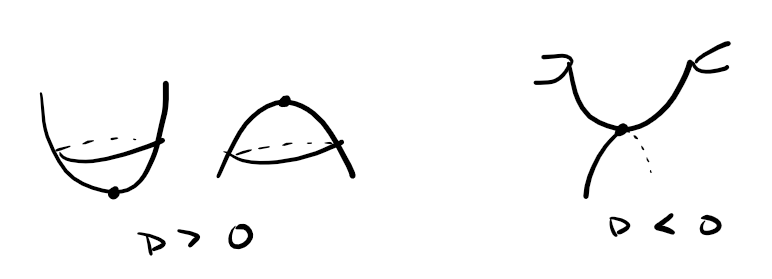
\includegraphics[width=120mm]{Images/2nd-der-test}
\caption{Critical points with $D>0$  (left) and $D<0$ (right)}
\label{fig-2nd-der-test}
\end{figure}

Also, it's worth mentioning that $D$ is still a two-variable function of $x$ and $y$, as each of the partial derivatives of $f$ are. The following theorem tells us how to use this to determine the behavior of a function at a critical point.



\begin{thm}[Second derivative test] Suppose we have a function $f=f(x,y)$ and a critical point $(a,b)$ for $f$. Let $D$ be the Hessian determinant of $f$ as above. Then the following holds:
\begin{itemize} 
	\item If $D(a,b)>0$ then $f$ has a maximum or a minimum depending on the following:
		\begin{itemize}
			\item If $f_{xx}(a,b)>0$ then $(a,b)$ is a \textit{minimum}
			\item If $f_{xx}(a,b)<0$ then $(a,b)$ is a \textit{maximum}
		\end{itemize}
	\item If $D(a,b)<0$ then $f$ has a saddle point at $(a,b)$; this is neither a max nor a min.
	\item If $D(a,b)=0$ the test is inconclusive; $(a,b)$ could be a max, min, saddle point, or something else entirely; further exploration is needed.
\end{itemize}
\end{thm}

\begin{remark}We'll focus primarily on the first two cases, as the third requires a more in-depth analysis of the function at hand. In the case $D>0$ note the similarity to the second-derivative test for one-variable functions, $f_{xx}$ is a measurement of concavity of $f$, but in the $x$-direction only. In fact, in this case, you could just as well replace $f_{xx}$ by $f_{yy}$ as they will have to have the same behavior (\textit{why is this? you can actually figure this out by looking at the expression for $D$}).\end{remark}

\subsection{Steps for finding local extrema}
The process for finding local extrema then is the following: First find critical point, then use the second derivative test to determine whether each critical point is a max, min, or saddle point. If the test is inconclusive at any of the critical points you can try to use a graph to determine any further information about the behavior of the function at that point.

\subsection{Global extrema}

Recall that, in contrast with a \textit{local} extremum, a \textit{global} extremum of a function is the largest/smallest overall value taken by that function on the given domain. Not all functions have global extrema on all domains, and both parts (that is, the function and the domain) are equally important in finding global extrema. 

For a function $f=f(x)$ the process goes as follows: Suppose $f$ is a function defined on some interval $[a,b]$---that this is a closed interval (contains the endpoints) is important here---then, any global extrema can occur at one of two types of places:
\begin{itemize}
	\item At a critical point
	\item At one of the endpoints of the interval
\end{itemize}

To find it, you simply plug these values into the function and ask which is the largest/smallest. To find global extrema for a function of two variables we rely on the following observation:

\begin{thm}[Condition for existence of global extrema for functions of two variables)]Suppose that $f=f(x,y)$ is a (continuous) function of two variables defined on some domain $D$ in the $xy$-plane. If $D$ is \textit{closed} then $f$ must attain a global maximum and minimum on its domain
\end{thm}

\begin{remark} The precise definition of what makes a region closed is not entirely necessary: it's sufficient for us to know that $D$ contains all curves that make up its boundary. For instance the box $-1\leq x\leq 1, -1\leq y\leq 1$ is closed as it contains the boundary line segments, while the open box $-1<x<1, -1<y<1$ does not and is therefore not closed (see Figure \ref{fig-squares}).
\begin{figure}[h]
\centering
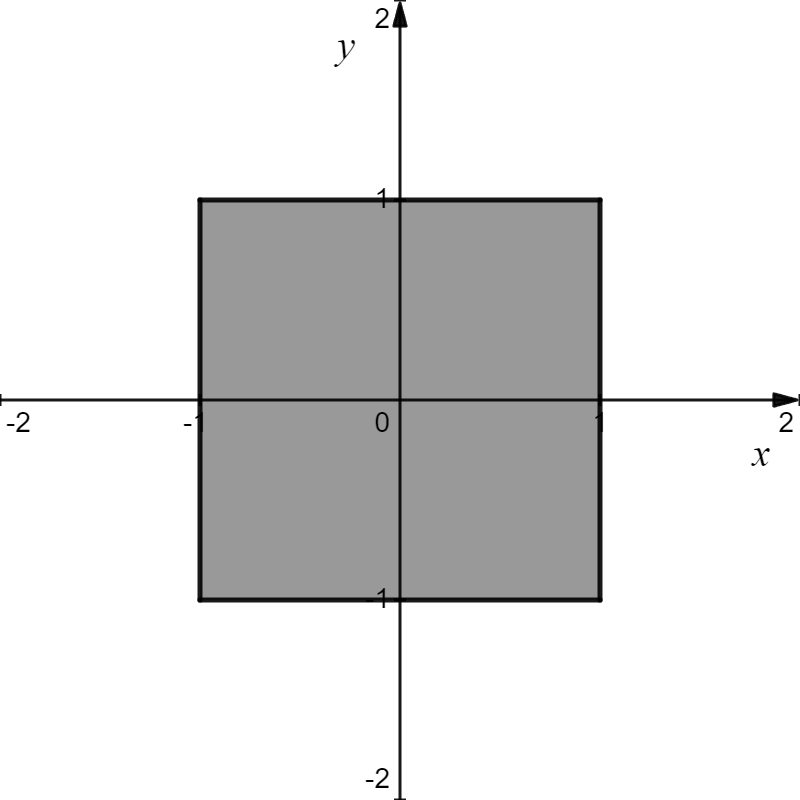
\includegraphics[width=50mm]{Images/closed} \qquad \qquad \qquad 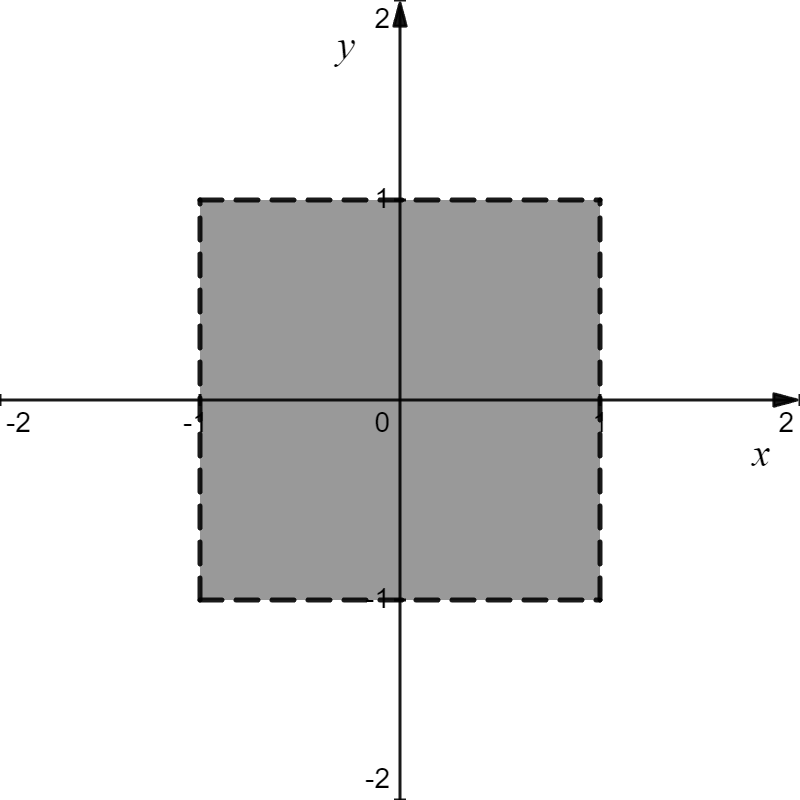
\includegraphics[width=50mm]{Images/open}
\caption{Closed square (left), open square (right)}
\label{fig-squares}
\end{figure}
\end{remark}

\subsection{Finding global extrema of a two-variable function}Suppose $f=f(x,y)$ is a (differentiable) function of two variables defined on a closed region $D$ in the $xy$-plane. Then, the global max/min of $f$ must occur at one of the following places:

\begin{itemize}
	\item At a critical point in the interior of $D$ (i.e., not on the boundary)
	\item At a critical point along the boundary
	\item At an intersection of any two boundary components
\end{itemize}

The first is simple enough, find critical points as you would for local extrema and check that they lie inside the region $D$. 

For the second, we must \textit{parametrize} any component of the boundary, plug that parametrization into the function $f$, and treat it as a one-variable function. If $D$ is the box region above, and $f(x,y)=x^2y$, this would amount to parameterizing each of the four line segments that make up the boundary of the square and plugging each into $f$. For instance, one such component is $r(t)=(t,1)$ for $-1\leq t\leq 1$. So $f(r(t))=t^2\cdot 1=t^2$, and then you find critical points for this function on the domain $[-1,1]$. 

Lastly, any ``corner point'' where two different parametrization is automatically a point where a max/min could occur. For the square then the four corners $(\pm 1, \pm 1)$ all must be checked for global extrema. 


This is a long process, and gets longer as the number of variables of the function goes up. In section \ref{LM}, we'll learn about Lagrange multipliers---a technique that can save us some effort here by using the gradient in a clever way.

\subsection{Exercises}
\begin{enumerate}[label=\arabic*.]
\item Determine any local extrema and saddle points for the following functions:

\begin{enumerate}
	\item $f(x,y)=x+3+xy+x^2$
	\item $f(x,y)=x^3-y^2$
	\item $f(x,y)=xe^y$
	\item $f(x,y)=y\sin(x)$
\end{enumerate}

\item Let $R$ be the triangle in the $xy$-plane with vertices at $(0,0)$, $(0,4)$ and $(5,0)$. In this problem we will find the global extrema of the function $f(x,y)=xy-x-3y$ on $R$.

\begin{enumerate}
	\item For each of the lines that make up the boundary of $R$ (i.e., edges of the triangle) give a parametrized function for that line
	\item Use the parametrization from part a. to any critical points of $f$ along each of the edges of its domain
	\item Find any critical points on the interior of $R$ by solving for where $f_x=f_y=0$ within the region. 
	\item Use the points obtained from parts b. and c., along with the three vertices of the triangle, to check for global extrema of $f(x,y)$ on $R$
\end{enumerate}

\item Find the global extrema of $f(x,y)=x^2+2y^2-x$ on the region given by the disc $x^2+y^2\leq 4$ in the following steps
\begin{enumerate}
	\item Find any critical points of $f$ on the interior of the disc $x^2+y^2<4$
	\item The boundary of the disc is given by $x^2+y^2=4$. Use the substitution $y^2=4-x^2$ in $f(x,y)$ to solve for any critical points of $f$ on the boundary.
	\item Using the points from parts a. and b., solve for any global extrema of $f$ on $R$
\end{enumerate}

\item Find the points on the surface $x^2-yz=5$ closest to the origin. \textit{Hint: The distance from $(x,y,z)$ to the origin can be computed as $d(x,y,z)=x^2+y^2+z^2$. Use that if $(x,y,z)$ is on the surface then $x^2=5+yz$, to make a substitution into $d(x,y,z)$ and minimize the resulting function of two variables.}

\item \textit{True or False}. Determine if the following statements are true or false. Give a brief justification of your answer. Let $D$ be the Hessian determinant from \eqref{Hess-det}

\begin{enumerate}
	\item If $D(a,b)>0$ then $f$ has a local extrema at $(a,b)$
	\item If $f=f(x,y)$ has a global maximum at a point $(a,b)$, then $D(a,b)>0$
	\item Any continuous function $f=f(x,y)$ with domain given by $x^2+y^2\leq 1$ must have a global minimum
	\item If $(a,b)$ is a critical point of $f$ with $f(a,b)=0$ and $D(a,b)<0$. Then $f$ must attain both positive and negative values on its domain.

\end{enumerate}
\end{enumerate}

Selection additional exercises: \textit{Stewart} section 14.7

\section{Lagrange multipliers} \label{LM}

The strategy of \textit{Lagrange multipliers} is a convenient way to find maximum or minimum values of functions of several variables given some list of constraints. The simplest case is when you want to find extrema of a function $f=f(x,y)$ along some level curve $g(x,y)=k$ of of another function $g$.

The technique comes from the following observations: \begin{itemize} 
	\item $\nabla f$ points in the direction of greatest increase of $f$
	\item $\nabla g$ is always perpendicular to any level curve of $g$
	\item If the function $f$ obtains an extremum along a level curve of $g$, then $\nabla f$ and $\nabla g$ must be parallel. 
\end{itemize} 
\begin{remark}For the last condition: assume at a point $(a,b)$ on $g(x,y)=k$, that $\nabla f$ and $\nabla g$ are not parallel. Let $u$ be a tangential direction to the level curve $g(x,y)=k$. Since $u\cdot \nabla g=0$ then we cannot have $u\cdot \nabla f=0$ as well (otherwise $\nabla f$ and $\nabla g$ would be parallel). So, $D_u f$ is not 0. Suppose that $D_uf>0$ then $D_{-u}f<0$ and so $f$ cannot have an extremum at this point. A similar argument holds if $D_uf<0$. Therefore, $f$ can attain a maximum or minimum at $(a,b)$ only if $\nabla f(a,b)$ is parallel to $\nabla g(a,b)$.
\end{remark}

Piecing these together we get a system of equations:
\[
 	f_x=\lambda g_x, \qquad
	f_y=\lambda g_y, \qquad
	g(x,y)=k
\]
where the first two come from setting $\nabla f=\lambda \nabla g$ (i.e., insisting that the two vectors be parallel), and the third is the particular level curve of $g$ that is desired. In general, the method of Lagrange multipliers is applied as follows:




\begin{thm}[Condition for extrema via Lagrange multipliers] Let $f$ and $g$ be functions of two variables and let $k$ be a constant such that the level curve $g(x,y)=k$ is contained within the domain of $f$. Then, any global extrema of $f$ along the level curve $g(x,y)=k$ must occur at a point $(a,b)$ such that
\begin{equation} \label{LM-1} \nabla f(a,b)= \lambda \nabla g(a,b) \qquad \text{and} \qquad g(a,b)=k \end{equation}
where $\lambda$ is a constant. Notably, \eqref{LM-1} gives a system of equations we can solve to try to find all global extrema of the given function. 
\end{thm}
\begin{figure}[h!]
\centering
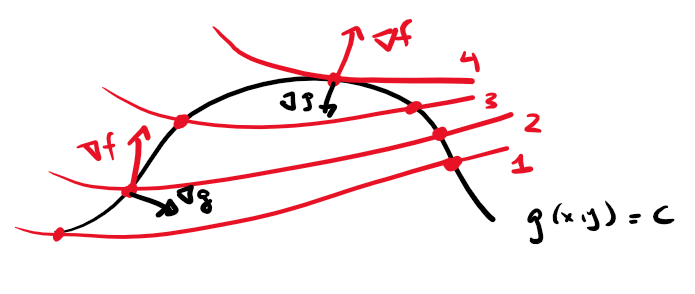
\includegraphics[width=100mm]{Images/LM}
\caption{Gradient vectors for a two variable function $f$ and constraint curve $g(x,y)=c$}
\label{fig-LM}
\end{figure}

\begin{example}Suppose we want to find the maximum of $f(x,y)=x^2+2y^2$ along the curve $x^2+y^2=1$. The second equation gives $g(x,y)=x^2+y^2$ which results in the equations\[ 
	2x=\lambda 2x, \qquad
	4y=\lambda 2y, \qquad
	x^2+y^2=1\]
Typically these systems can be quite tricky to solve, but it's always possible to solve for $\lambda$ two ways, equating $x$ and $y$. Sometimes you might find it easier to solve for $x,y$ in terms of $\lambda$, and use these in the constraint function to find what values of $\lambda$ are possible. In either case, here we find solutions $(x,y)=(\pm 1,0)$ and $(0,\pm 1)$ (note that each has a value of $\lambda$ attached to it, but we don't actually care what that value was). Since these are the only critical points of $f$ found in the domain, we just evaluate $f$ at each to find that $f(\pm 1,0)=1$ are the minima and $f(0,\pm 1)=2$ are the maxima. 
\end{example}

\begin{remark}Importantly this gets away without having to parametrize boundary components like we did before. The technique also extends readily to finding extrema of a function $f=f(x,y,z)$ along a level \textit{surface} $g(x,y,z)=k$ of another function $g$. Using the same idea from \eqref{LM-1} we get a system of \textit{four} equation system of four variables, \[\nabla f(a,b,c)=\lambda \nabla g(a,b,c), \quad g(a,b,c)=k\] that any extrema $(a,b,c)$ of $f$ must satisfy. Even more better, this technique can be further modified to find extrema of $f$ with two constraint functions (or even more generally a function of $n$ variables with $m<n$ constraints).\end{remark}

\subsection{Exercises}
\begin{enumerate}[label=\arabic*.]
\item Use Lagrange multipliers to find all extreme values of $f$ along the given constraint.

\begin{enumerate}
	\item $f(x,y)=x^2-y^2$, $x^2+y^2=1$
	\item $f(x,y)=xe^y$, $x^2+y^2=2$
	\item $f(x,y,z)=xy^2z$, $x^2+y^2+z^2=4$
	\item $f(x,y,z)=e^{xyz}$, $2x^2+y^2+z^2=24$
\end{enumerate}

\item Show that $f(x,y)=x^2+y^2$ has no maximum value along the level curve $xy=1$. Then use Lagrange multipliers to find its minimum value.

\item Use Lagrange multipliers to show that the largest rectangle with a given perimeter is a square. Can the same idea be used to show that the same to show that the largest rectangular prism with a given surface area is a cube?

\item Use Lagrange multipliers to find the maximum value of $f(\alpha, \beta,\gamma)=\cos \alpha \cos\beta \cos\gamma$ given that $\alpha, \beta$ and $\gamma$ are the three inner angles of a triangle. (\textit{Hint: the inner angles of a triangle always add to $\pi$.})

\item *Let $n\geq 2$ and set $f(x_1,x_2,\dots, x_n)=\sqrt[n]{x_1x_2\cdots x_n}$. Use Lagrange multipliers to find the maximum value of $f$ given that all inputs $x_i$ are positive numbers and $x_1+\cdots+x_n=k$ for some constant $k$. 

Use this to show that \[ \sqrt[n]{x_1x_2\cdots x_n} \leq \dfrac{x_1+x_2+\cdots+x_n}{n} \] for all positive numbers $x_1,\dots, x_n$\footnote{This last inequality is often called the \href{https://en.wikipedia.org/wiki/AM\%E2\%80\%93GM_inequality}{AM-GM inequality}, i.e., that the arithmetic mean of $n$ numbers is always greater than the geometric mean $\sqrt[n]{x_1x_2\cdots x_n}$}.

\end{enumerate}
Suggested additional exercises: \textit{Stewart} section 14.8


\section{**Gradient descent}

Gradient descent is a very general optimization strategy found within a variety of applications from pure mathematics to machine learning and neural networks. Here we'll pick up some basic approaches to the technique, but know this is just the tip of the iceberg in terms of the subject.

Suppose you have a system of $n$ equations in $n$ variables, for instance consider the following $2\times 2$ system:
\begin{align} 2x-y & =1 \nonumber \\
x+y &=2 \label{sys-1} \end{align}
Since the equations in \eqref{sys-1} are linear in the variables $x$ and $y$, we can use basic ideas from linear algebra to show that this system has just the one solution $(x,y)=(1,1)$. In particular, it's possible to solve any $n\times n$ system of linear equations without too much pain.

\subsection{Nonlinear systems of equations}
But what if the equations are nonlinear? For instance, let's consider the $2\times 2$ system 
\begin{align}
2\cos(y-1)+2x&=1 \nonumber \\ y-\cos(x) &=3 \label{sys-2} \end{align}
Attempting to isolate $x$ or $y$ and proceed as before \textit{may} be possible, but is definitely no longer as straightforward. Here comes our idea of gradient descent. Recall the following fact (see theorem \ref{gradient-properties}).

\begin{fact}For a differentiable function $f$ of $n$ variables, the gradient $\nabla f$ is a vector in $\mathbf{R}^n$ which points in the direction of greatest increase of $f$. \end{fact}

One corollary is that the \textit{negative} gradient $-\nabla f$ points in the direction of greatest \textit{decrease} of $f$\footnote{Why is this? it follows from the formula for the directional derivative $D_uf=\nabla f \cdot u$}. This leads us to the question: \textit{Given an $n\times n$ system of equations, what function gives us a measure of ``accuracy'' for a solution?} There's possible many answers but an obvious choice would be to measure the \textit{error} of a guess solution in terms of the distance formula (which is essentially what we do below). 

\begin{defn} Let $f,g$ be differentiable functions of two variables and consider the system $f(x,y)=g(x,y)=0$. Define the \textbf{error} function $E$ by \begin{equation} \label{error} E(x,y)=\dfrac{1}{2} \left( f(x,y)^2 + g(x,y)^2 \right)\end{equation} \end{defn}

Note that this error function can just as well be defined for a system of $n$ equations with $n$ variables. If $(x,y)$ is a solution to the system $f(x,y)=g(x,y)=0$ then $E(x,y)=0$, otherwise $E(x,y)>0$. So, what $E$ measures is a (rescaling) of the distance from a guess solution to an \textit{actual} solution of the given system. 

\begin{example} \label{gd-ex}Let's consider the system \eqref{sys-1}. Moving the $1$ and $2$ to the other side, we get $f(x,y)=2x-y-1$ and $g(x,y)=x+y-2$, and so  \[ E(x,y)= \dfrac{1}{2} \left( (2x-y-1)^2 + (x+y-2)^2 \right)=\dfrac{1}{2} \left( 5 x^2 - 2x y - 8 x + 2y^2 - 2y + 5\right) \]
Taking gradients, we find \[ \nabla E(x,y) = \left( -4 + 5 x - y, -1 - x + 2 y\right)\]
Let's interpret this gradient. Suppose we have an initial guess solution $(x_0,y_0)=(0,0)$ to this system of equation. It's not right, as $E(0,0)=5/2$, but  since $-\nabla E$ always points in the direction of \textit{greatest decrease} of $E$ we can improve this guess by taking a small step in the $-\nabla E(0,0)$ direction. Let $\epsilon$ be a small number (we'll decide a good value for it later) and set \[ (x_1,y_1)=(x_0,y_0) - \epsilon \nabla E(x_0, y_0)\]  The hope would be that by taking a small enough step in this direction, we simply go toward a minimum of $E$. Let's set $\epsilon=0.1$ for now. Since $\nabla E(0,0)=(-4,-1)$ 
\[ (x_1,y_1)=(0,0)- 0.1 (-4,-1)=(0.4, 0.1)\]
Let's check what happened to the error: we now have \[E(x_1,y_1)=E(0.4, 0.1)=7/6<5/2=E(x_0,y_0).\] So, this improved guess is \textit{closer} to being a solution than our first guess of $(0,0)$, but still not quite there. The key here is that we can iterate this computation, keeping $\epsilon=0.1$ we have \begin{align*} (x_2,y_2) &= (0.4,0.1) - 0.1 (-2.1, 1.2)=(.61,.22) \\ 
(x_3,y_3) &= (.61,.22) -0.1 (-1.17, -1.17) = (0.727, 0.337)\end{align*}
with errors $E(x_2,y_2)= 0.68445$ and $E(x_3,y_3)=0.444892$, so our approximations continue to become closer to a solution to the given system. Repeating this process a few more times, we expect to converge to the known solution of $(1,1)$---or at least become \textit{close enough} to it---where close enough can be quantified in terms of the error function (\href{https://msoe.box.com/s/lkjin287s0ahd7dnecyb7t3pefqzrf0d}{here} is my Excel spreadsheet with these calculations, with these initial values after 20 iterates we have an error less than 0.001---this could be improved with a more informed choice of step size). 
\end{example}

Noteworthy is that we did all of the above algebraically (meaning, without having to know pictures of the functions involved), and while the computations become a bit tedious to do by hand, the process can easily be implemented with whatever computational coding language you feel most comfortable with.


\begin{defn}[Gradient descent ``formula"] Given differentiable functions of two variables $f,g$ let $E$ be the error function as defined in \eqref{error}. Given an initial guess solution $(x_0,y_0)$ and ``step size" $\epsilon$, we can inductively define a sequence $(x_n,y_n)$ of approximations to the system $f(x,y)=g(x,y)=0$ as follows. \begin{equation} (x_{n+1},y_{n+1})=(x_{n},y_{n})-\epsilon \nabla E(x_{n},y_{n}) \qquad ( n \geq 0) \label{gd} \end{equation} 
\end{defn}

\begin{remark}. There are many subtleties here, for instance: what makes a ``good'' step size $\epsilon$? When do we know to terminate this procedure? If the system has many solutions, how can we predict which solution this process will converge to? These are all great questions but quickly go beyond the scope of what we're trying to accomplish. For us, a step size will be given at the onset, but know that it's possible to determine ``good'' choices of $\epsilon$ based on properties of the functions which make up the given system.  (Also note you might want to allow the step size to vary with $n$, but that's not important at the moment). \end{remark}

\subsection{Using gradient descent on a nonlinear system} Let's go back to our nonlinear system \eqref{sys-2} from before. This has $f(x,y)=2\cos(y-1)+2x-1$ and $g(x,y)=y-\cos(x)-3$. Computing, we get \begin{align*} E_x(x,y)&= -2 + 4 x + 4 \cos(1 - y) + (-3 + y - \cos(x)) \sin(x) 
 \\ E_y(x,y)&= -3 + y - \cos(x) + 2 (-1 + 2 x + 2 \cos(1 - y)) \sin(1 - y) \end{align*}

A potential nightmare to work with, but let's give it a shot (now is a great time to use a calculator/computational software). Without thinking too hard, an initial guess could be $(x,y)=(1,2)$, in which case $E(1,1)\approx 3.351
$. Not great, but we can improve it. With a step size of $\epsilon =0.25$ we can calculate \begin{align*} 
(x_1,y_1)&=( 0.283,	3.260) && E= 1.6983 \\
(x_2,y_2)&= (1.185,	2.777) && E=0.6395 \\
(x_3,y_3)&=(0.843,	3.396) && E= 0.3420 \\ 
 (x_4,y_3)&=(1.285,	3.198) && E= 0.0817\\
(x_5,y_5)&=(1.107,	3.379) && E=0.0292\\
(x_6,y_6)&=(1.238,	3.316) &&E= 0.0073
\end{align*}
(These are truncated values: Again, I did this in Excel, you can use my spreadsheet \href{https://msoe.box.com/s/lkjin287s0ahd7dnecyb7t3pefqzrf0d}{here} if you want, or make a better version. If you use my version, you can play around with different values of $\epsilon$ (epsilon) and the starting $x$ and $y$ coordinates). Note how $E$ decreases with each iteration. If we desired to get within an error of $0.01$ then by the sixth iterate we're there. 


Since the functions we're working with here are only in two variables, we can still get some visual info about what is happening. \href{https://www.math3d.org/4J9C11cPD}{Here} is a Math3D plot of the error for function $E$ of the given two variable system. We can see visually we're converging to the global min where $E(x,y)=0$ in the first quadrant, which if we let our approximation machine run long enough would begin $(1.207...,3.356...)$. Furthermore, we can actually determine this is the \textit{only} solution by appreciating the graphs of the two functions  in Figure \ref{fig-grad-curves} and noting that this could be the only possible crossing of the two sinusoids.

\begin{figure}[h!]
\centering 
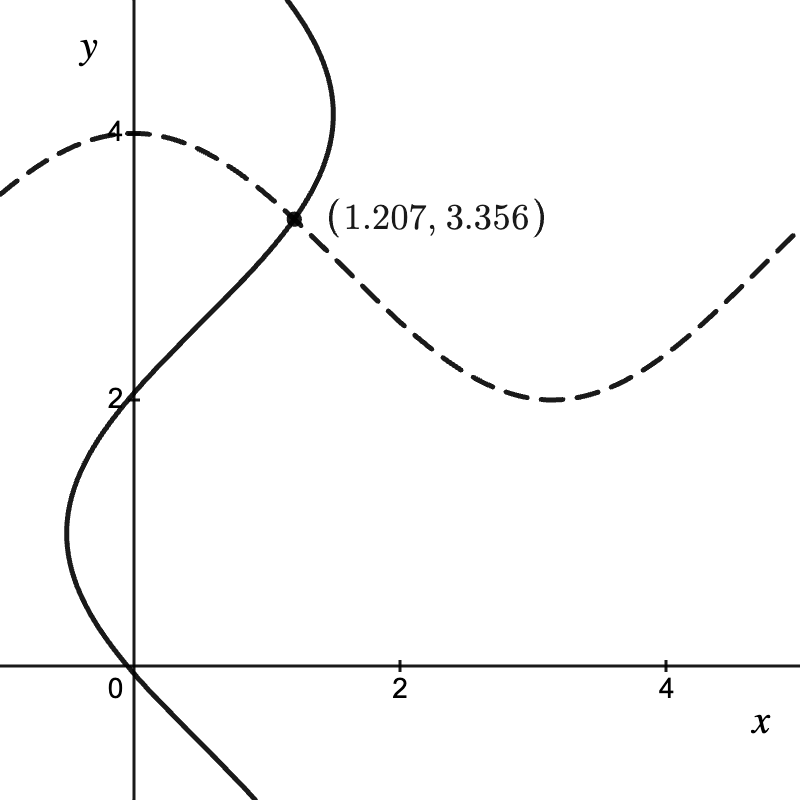
\includegraphics[width=60mm]{Images/ws14-sol-2}
\caption{Curves $f(x,y)=0$ (bold) and $g(x,y)=0$ (dashed)}
\label{fig-grad-curves}
\end{figure}


\begin{remark}While we benefit from the simplicity of $2\times 2$ systems for this example, one main benefit of this process is that \eqref{gd} can easily be modified to an arbitrary $n \times n$ system of equations, where the supplementary graphs of the functions are difficult if not impossible to parse meaningfully. In particular, if you have software that can effectively calculate derivatives and approximate basic elementary functions (e.g., $\sin$, $\cos$, etc) then you can ``easily'' implement this kind of idea and offload the many tedious calculations onto the computer (there are many python packages for this type of work).\end{remark}

Gradient descent is not limited to solving/approximating solutions to nonlinear systems of equations either: one common use to the measure the error of a neural network's prediction against some reliable testing data, adjusting the weights of each neuron according the a similar gradient descent formula as \eqref{gd}. But this is a story for another time.

\begin{warning}With any iterative approximation algorithm there's always the nagging question of ``when do we terminate this algorithm?" Since it's unlikely that our approach will land us \textit{exactly} at a solution to the system, if we set a level of acceptable error at the onset, we can safely terminate whenever you find a point within that threshold. But what if that's never achieved? For instance, the algorithm might get ``stuck" in a local min of $E$ somewhere far off from an actual solution and never hit the desired error threshold. It's also worth mentioning that this method will find you \textit{a} (or several) solution(s), but that it is difficult/impossible still to determine if it has found \textit{all} solutions to the given system.\end{warning}

\subsection{Exercises}
\begin{enumerate}[label=\arabic*.]

\item Modify the technique from \eqref{gd} to work with three variable functions, then approximate a solution to the following system of equations using a step size of $0.001$ (you should probably use some software).  \begin{align*}
	&3x-\cos(yz)=3/2 \\
	&4x^2-625y^2 +2y=1\\
	&e^{-xy}+20z+10\pi/3=1
\end{align*}

\item One useful application to data science is finding curves of best fit to a collection of data. Given a set of points $(x_i,y_i)$ for $i=1,\dots,n$ in the $xy$-plane, we can use gradient descent to approximate the linear regression; i.e., the line of best fit of the form $y=mx+b$. Here, the values of slope $m$ and $y$-intercept $b$ will be our values to approximate; so $E=E(m,b)$ is a function of these quantities given by \begin{equation} E(m,b)= \dfrac{1}{2} \sum_{i=1}^n \left( mx_i +b -y_i \right)^2\end{equation} 
(note that this is the distance from ``predicted'' $y$-value $m x_i+b$ to the given $y$ value $y_i$.)
\begin{enumerate}
	\item Show that $\nabla E$ has the form \begin{equation} \nabla E(m,b)=\left( \sum_{i=1}^n x_i (mx_i+b-y_i), \sum_{i=1}^n mx_i +b-y_i\right)\end{equation}
	\item Use the gradient descent method outlined in \eqref{gd} with a step size of $\epsilon=0.1$ to approximate the linear regression to the collection of points \[\{ (1,2), (0,1), (3,6), (-1,-4), (4,7), (5,12), (-3,-5)\}\] to within an error of $0.01$.
\end{enumerate}

%Expressions of such type are called
\item An ``optimal'' choice for $\epsilon$ at the $n$-th iterate of \eqref{gd} can be given as follows (under some moderate assumptions of the error function $E$). Let $\delta_{x,y}$ and $\delta_{E}$ be the displacement vectors given by \[ \delta_{x,y}=(x_n, y_n)-(x_{n-1},y_{n-1}) \qquad \qquad \delta_{E}=\nabla E(x_n,y_n)-\nabla E(x_{n-1},y_{n-1})\]
Then, $\epsilon$ to find $(x_{n+1},y_{n+1})$ can be set to \begin{equation} \epsilon = \left| \dfrac{ \delta_{x,y} \cdot \delta_E }{\delta_E \cdot \delta_E} \right|\end{equation} where $\cdot$ is the dot product of vectors, and absolute value is taken to ensure that $\epsilon>0$. Use this to chose the ``optimal'' $\epsilon$ to find $(x_2,y_2)$ for the system \eqref{sys-1}. Was our choice of $\epsilon=0.1$ good enough?
\end{enumerate}

\section{Double integrals}


Our main focus is now on integral calculus of multivariable functions. We start with double integrals: as we'll see, the difficulty here is in setting up the integrals. Most of the calculations are just multiple passes through integration techniques you may recall from Calc 2. It's not a bad idea to brush up on some of these skills, though as far as calculations in this course go it's unlikely we'll have to use a technique more sophisticated than integration by parts for most problems. 


First, we have to define what type of regions are suitable for integration. Recall that a region $R$ in $\mathbf{R}^2$ is \textbf{closed} if it contains all curves that make up its boundary, and \textbf{bounded} if it doesn't ``go off to $\infty$" in any direction\footnote{It's sufficient to say that a region is \textit{bounded} if it is contained entirely within the disc $x^2+y^2=r^2$ for some real number $r$}. 


\begin{defn}[The double integral] Let $f=f(x,y)$ be some two variable function which is defined and continuous on some domain $R$ in the $xy$-plane. The \textbf{double integral} of $f$ over $R$ is written \begin{equation} \iint_R f\,dA \label{int-dA} \end{equation} 
and is equal to the ``continuous sum" of $f$ over $R$.\end{defn}

\begin{remark}
Interpreted differently, the definite integral $\int_R f\,dA$ is the \textit{net signed volume} between the surface $z=f(x,y)$ and tthe $xy$-plane (within the region $R$). Here, \textbf{signed} means that stuff above the $xy$-plane is to be treated as positive volume, and stuff below the $xy$-plane negative. This should be the ``evident'' analog of a definite integral from one-variable calculus (regions formed by surfaces produce \textit{volumes}, regions formed by curves create \textit{areas})

%he symbol $\iint_R f\,dA$ is a number that number is the volume of the solid 3d region in question. As with definite integrals of one variable, the adjectives \textit{net signed} applied to volume tell us that ``stuff'' above the $xy$-plane is to be treated as positive volume and ``stuff'' below the $xy$-plane is to be treated as negative; \textit{underneath} is meant to be interpreted as ``between the graph of $z=f(x,y)$ and the $xy$-plane''. 

\end{remark}

The notation $dA$ is called the \textbf{area differential} and \eqref{int-dA} can be said as ``the (double) integral of $f$ with respect to area''. This doesn't yet tell us how to calculate a double integral, but we'll get there shortly.  As we'll see, looking at these differentials first is a good check for what kind of multivariable integral we're trying to evaluate.

\subsection{Riemann sums}
 It's possible to define $\iint_R f\,dA$ as a limit of Riemann sums, but this is expectedly as (if not more) tedious than you might recall the similar discussion for one variable functions being, so we wont go down this route.\footnote{The idea would be to chop the domain $R$ into a bunch of rectangular pieces $R_i$, select a point $(x_i,y_i)$ from each piece, and approximate the volume under $z=f(x,y)$ on this piece by the volume of the rectangular prism formed with base $R_i$ and height $f(x_i,y_i)$. Fubini's theorem (Theorem \ref{thm-fubini}) is really the statement that if $f$ is continuous that these sums converge regardless of choice of basepoint, and that moreover the double integral is computed by iterated one-variable integrals. 
 
I won't make you do anything with calculating multivariable Riemann sums but it's nice to know this \textit{can} be done. Never write off Riemann sums, they are extremely useful as an approximation technique, just not typically something you'd do by hand.}

\subsection{Iterated integrals}
Looking at \eqref{int-dA} it's reasonable then to wonder: \textit{how do we actually calculate this integral}? This is where \textit{iterated integrals} come into play. The idea is fairly simple: if we want to cover the whole area of a domain $R$ we can simply first ``sweep'' across one variable, then the other.

\begin{thm}[Fubini's theorem] \label{thm-fubini}Let $f=f(x,y)$ be a two variable function defined and continuous on a rectangular region $R$ given by $a\leq x\leq b, c\leq y\leq d$ (for constants $a,b,c,d$) in the $xy$-plane. Then: \begin{equation} \label{int-dxdy} 
	\iint_R f\,dA= \int_a^b \int_c^d f(x,y) \,dy \,dx= \int_c^d \int_a^b f(x,y) \,dx\,dy
\end{equation}
\end{thm}
We often can interpret this as an equivalence of differentials: \begin{equation} \label{differentials-1} dA=dx\,dy =dy\,dx\end{equation} which will fit in nicely with our discussion about change of variable substitutions in double and triple integrals. Note here that the expressions in \eqref{int-dxdy} should be parsed as \[ \int_a^b \left(\int_c^d f(x,y) \,dy\right) \,dx  \text{\quad and \quad } \int_c^d \left( \int_a^b f(x,y) \,dx \right) \,dy \] idea being that the inner integrals add up all the ``stuff'' along $y$ (resp. $x$) first as a function of $x$ (resp. $y$). These types of expressions are called \textbf{iterated integrals} and are our main tools for computing double (and triple and beyond) integrals. 

\begin{remark}When the domain region $R$ for a double integral is not simply a rectangle Fubini's theorem still applies, however, more work is needed is changing the bounds of integration upon swapping the order. For instance, when switching to $dx\,dy$ from $dy\,dx$ you may find that you need multiple integrals with different bounds to fully describe the region $R$. \end{remark}

\subsection{Exercises}
\begin{enumerate}[label=\arabic*.]
\item Evaluate the following iterated integrals

\begin{enumerate}
	\item $\displaystyle \int_0^1 \int_0^1 xe^y\,dx\,dy$
	\item $\displaystyle \int_0^1 \int_0^y e^x\,dx\,dy$
	\item $\displaystyle \int_{-1}^2 \int_{x^2}^{x}( x^2-y)\,dy\,dx$
	\item $\displaystyle \int_0^1 \int_0^{x^2} x\sin(y)\,dy\,dx$
\end{enumerate}

\item Evaluate the following double integrals on the indicate region $R$

\begin{enumerate}
	\item $\displaystyle \iint_R x^2\, dA$ where $R$ is bounded by $y=x, y=0$ and $x=1$. 
	\item $\displaystyle \iint_R y\,dA$ where $R$ is the region enclosed in the circle $x^2+y^2=1$ and line $x+y=1$ in the first quadrant
	\item $\displaystyle \iint_R (x-1) \,dA$ where $R$ is the region enclosed by $y=x$ and $y=x^3$ in the first quadrant
	\item $\displaystyle \iint_R xy\,dA$ where $R$ is the region enclosed by $y=\sqrt{x}, y=10-x$ and $y=0$
\end{enumerate}

\item Use a double integral to find the volume of the solid bounded above by the paraboloid $z=5-x^2-y^2$ above the square formed by $x=\pm 1, y=\pm 1$ in the $xy$-plane.

\item Express the following integrals as equivalent integrals with order of integration reversed 

\begin{enumerate}
	\item $\displaystyle \int_0^2 \int_0^{\sqrt{x}} f(x,y)\,dy\,dx$
	\item $\displaystyle \int_1^e \int_{\ln y}^{y} f(x,y)\,dx\,dy$
	\item $\displaystyle \int_0^1 \int_{\arcsin(y)}^{\pi/2} f(x,y)\,dx\,dy$
\end{enumerate}

\item The \textit{average value} of a function $f$ defined on region $R$ is given by \begin{equation} \bar{f}=\dfrac{1}{\text{area of $R$}} \iint_R f\,dA\end{equation}
Find the average value of $f(x,y)=\dfrac{1}{1+x^2}$ over the triangle $R$ with vertices $(0,0), (1,0), (0,1)$.

\item Find the volume of the tetrahedron with edges at $(0,0,0), (1,0,0), (0,1,0)$ and $(0,0,1)$. \textit{Hint: determine the equation of the plane which makes the top of the tetrahedron and use a double integral to find volume}. 


\item \textit{True or False}. Determine if the following statements are true or false. Give a brief justification of your answer. (For a,b, assume $f(x,y)$ is some integrable function on the given region.)

\begin{enumerate}
	\item $\displaystyle \int_a^b \int_c^d f(x,y)\,dy\,dx= \int_c^d \int_a^b f(x,y)\,dx\,dy$ for all constants $a,b,c,d$
	\item $\displaystyle \int_a^b \int_0^x f(x,y)\,dy\,dx= \int_0^x \int_a^b f(x,y)\,dx\,dy$ for all constants $a,b$
	\item $\displaystyle \int_0^1 \int_0^1 xy\,dx\,dy=\left( \int_0^1 x\,dx \right)\left( \int_0^1 y\,dy\right)$
	\item $\displaystyle \int_0^1 \int_0^{1-x} e^{-y^2}\,dy\,dx= \int_0^1 \int_0^y e^{-y^2}\,dx\,dy$
\end{enumerate}
\end{enumerate}


Suggested additional exercises: \textit{Stewart} sections 15.1, 15.2


\section[Polar coordinates]{Double integrals with polar coordinates}

In general, it's possible to ``exchange'' the $x,y$ coordinate system for an equally ``good'' one within a double integral, though the vastness of the collection of possible choices makes this often somewhat daunting. We learn one very useful substitution for double integrals: polar coordinates.

\subsection{Polar coordinates}
Recall that the polar coordinate system $(r,\theta)$ can be exchanged with $x,y$ coordinates as follows:
\begin{equation}x=r\cos\theta \qquad y=r\sin\theta \label{xy-to-polar} \end{equation}
The idea being that if $P=(x,y)$ is a point then $r$ and $\theta$ represent the distances from $P$ to the origin and angle from the positive $x$-axis (measure counterclockwise), respectively (see Figure \ref{fig-polar-coord}).

\begin{figure}[h!]
\centering
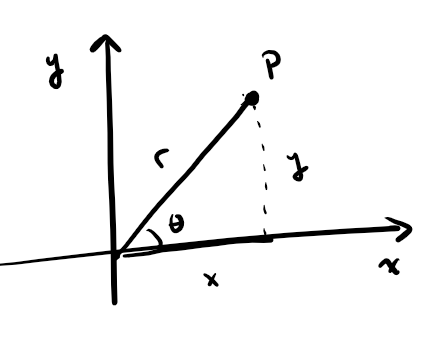
\includegraphics[width=60mm]{Images/polar-coord} 
\caption{Polar coordinates}
\label{fig-polar-coord}
\end{figure}

\subsection{Change of variables and the Jacobian}
In our language of multivariable functions, the polar substitution \eqref{xy-to-polar} can be interpreted as a \textit{function} $P\colon \mathbf{R}^2\to\mathbf{R}^2$ given by $P(r,\theta)=(x(r,\theta), y(r,\theta))$ where \[x(r,\theta)=r\cos\theta,\; y(r,\theta)=r\sin\theta\] What we want to figure out is how to get this substitution \eqref{xy-to-polar} involved with double integrals. Just like with one-variable functions, there is a rule for making a \textit{substitution} into an integral (i.e., a $u$-substitution). What we need to determine is how the differential ``$dA$'' will change when written in $r,\theta$ coordinates. This is called the \textit{Jacobian} (or more specifically, Jacobian determinant), and for polar coordinates is as follows:



\begin{defn}[Jacobian for polar coordiantes]
Let $x(r,\theta)=r\cos\theta,y(r,\theta)=r\sin\theta$ be the polar substitution functions. The \textbf{Jacobian matrix} for this substitution is given by \begin{equation} J=\begin{pmatrix} x_r & x_{\theta} \\ y_r & y_{\theta} \end{pmatrix}=\begin{pmatrix} \cos\theta & -r\sin\theta \\ \sin\theta & r\cos\theta\end{pmatrix} \end{equation}
	Correspondingly, the \textbf{Jacobian determinant} the determinant\footnote{Actually, it's the \textit{absolute value} of this determinant. When using polar coordinates, it's necessary to keep track of when the radius used to describe a region becomes negative. Whenever possible, use only positive radii in polar coordinates.} of this matrix \[ \det J=\cos\theta (r\cos \theta)-(-r\sin\theta)(\sin\theta)=r(\cos^2\theta+\sin^2\theta)=r\]
\end{defn}

The Jacobian determinant gives the appropriate ``scaling factor'' for dealing with how area changes with respect to the substituted functions in a double integral. 

\begin{thm}[Polar substitution for double integrals] Let $f=f(x,y)$ be a continuous function defined on a region $D$ in the $xy$-plane. Then \begin{equation} \label{polar-sub} \iint_D f\,dA= \iint_D f(r\cos\theta, r\sin\theta)\, r\, dr\,d\theta\end{equation} where, in the right hand side of the equation, $D$ also needs to be described in terms of the polar coordinates $r$ and $\theta$.
\end{thm}

\begin{remark}
	From \eqref{polar-sub} we get the equation of differentials (compare with \eqref{differentials-1}) \begin{equation} dA=r \,dr\,d\theta\end{equation} What this factor $r$ is doing is keeping track of how area has been distorted within this substitution. For instance, the ``polar rectangle'' $1\leq r\leq 2, 0\leq \theta\leq \pi/2$ has less area (viewed in the $xy$-plane) as the rectangle $3\leq r\leq 4, 0\leq \theta\leq \pi/2$ despite both of them having the same ``area'' in terms of $r,\theta$ coordinates (see Figure \ref{fig-polar-Jacob}). 
	
	\begin{figure}[h!]
	\centering
	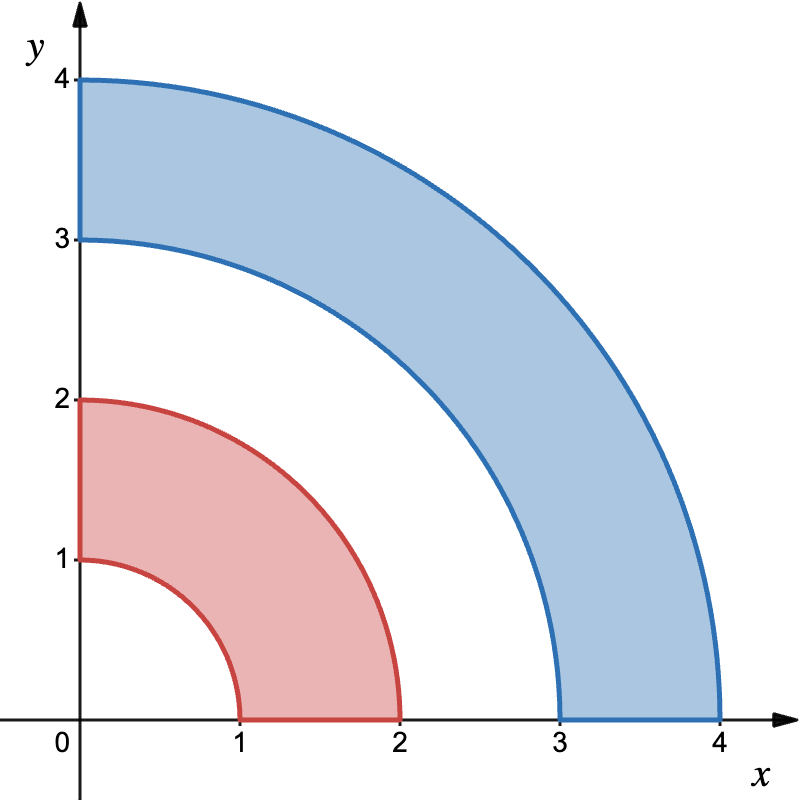
\includegraphics[width=60mm]{Images/polar-regions-area} \qquad \qquad 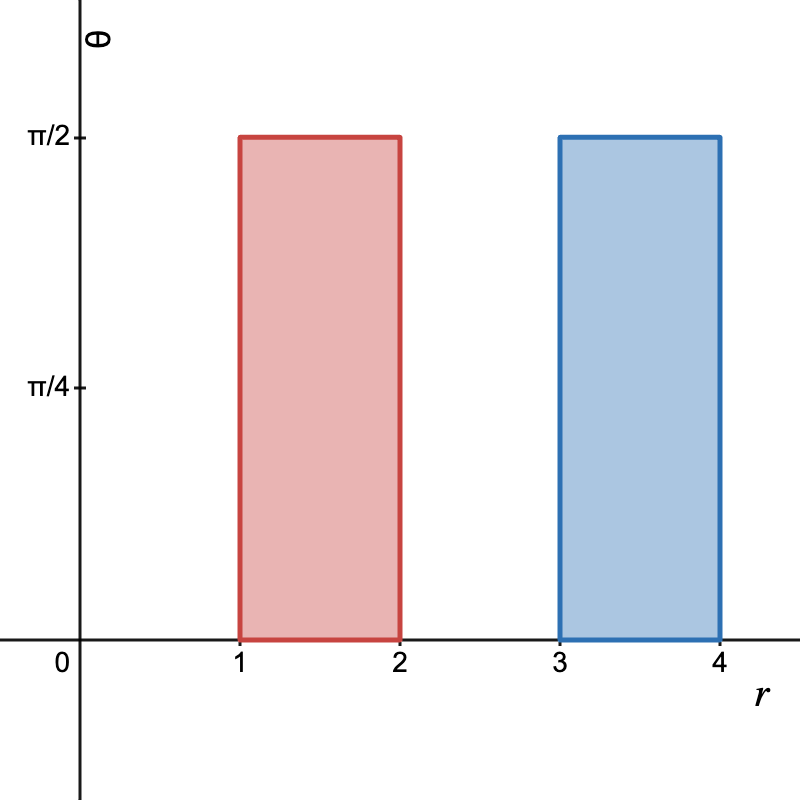
\includegraphics[width=60mm]{Images/rtheta-area}
	
	\caption{Polar rectangles $1\leq r\leq 2, 0\leq \theta \leq \pi/2$ (red) and $3\leq r\leq 4, 0\leq \theta \leq \pi/2$ (blue) which have the same area in the $r,\theta$ plane (right picture), but different areas in the $xy$-plane(left picture)}
	\label{fig-polar-Jacob}
	\end{figure}
	With this viewpoint, $dA$ is always ``area as we see it'' in the $xy$-plane, the right hand side is an integral in the variables $r,\theta$ which would make their own $r\theta$-plane, but we want to think of $r,\theta$ instead as how they encode areas in the $xy$-plane. Moreover, the order of integration $dr\,d\theta$ is more or less always this way. It's technically possible to reverse it, but geometrically it's much easier to think of $r$ as dependent on $\theta$ than vice-versa. 
	
\end{remark}
%%%ADD MORE TO HERE%%%

% The factor ``$r$'' in \eqref{polar-J} can look somewhat mysterious at first. It's best to think of it as a ``stretching factor'' of area when switching between the two coordinate systems. In general, there will be some ``stretching function'' when making a substitution of variables inside a double (or triple or beyond) integral (see problem 8 below).

\subsection{Exercises}
\begin{enumerate}[label=\arabic*.]
\item  Evaluate the following iterated integrals. If possible, describe the region of integration as a polar region in the $xy$-plane.
\begin{enumerate}
	\item $\displaystyle \int_0^{\pi} \int_0^{\sin \theta} r \cos \theta \, dr\,d\theta$
	\item $\displaystyle \int_0^{\pi/2} \int_0^{\sin \theta} r^2  \,dr\,d\theta$
	\item $\displaystyle \int_0^{\pi} \int_0^{\cos \theta} 3r^2 \, dr\,d\theta$
\end{enumerate}

\item  Use polar coordinates to evaluate the following double integrals

\begin{enumerate}
	\item $\displaystyle \iint_R \sin(x^2+y^2)\,dA$ where $R$ is the region inside the circle $x^2+y^2=1$
	\item $\displaystyle \iint_R \dfrac{1}{1+x^2+y^2}\,dA$ where $R$ is the region inside the circle $x^2+y^2 =4$ in the third quadrant
	\item $\displaystyle \int_0^1 \int_{-\sqrt{1-x^2}}^0 e^{x^2+y^2}\,dy\,dx$
\end{enumerate}

\item  Consider the region $R$ bounded by the polar function $r=\sin \theta$ and the Cartesian function $y=x$ as seen in the graph below. Use a double integral in polar coordinates to find the area of $R$

\[ 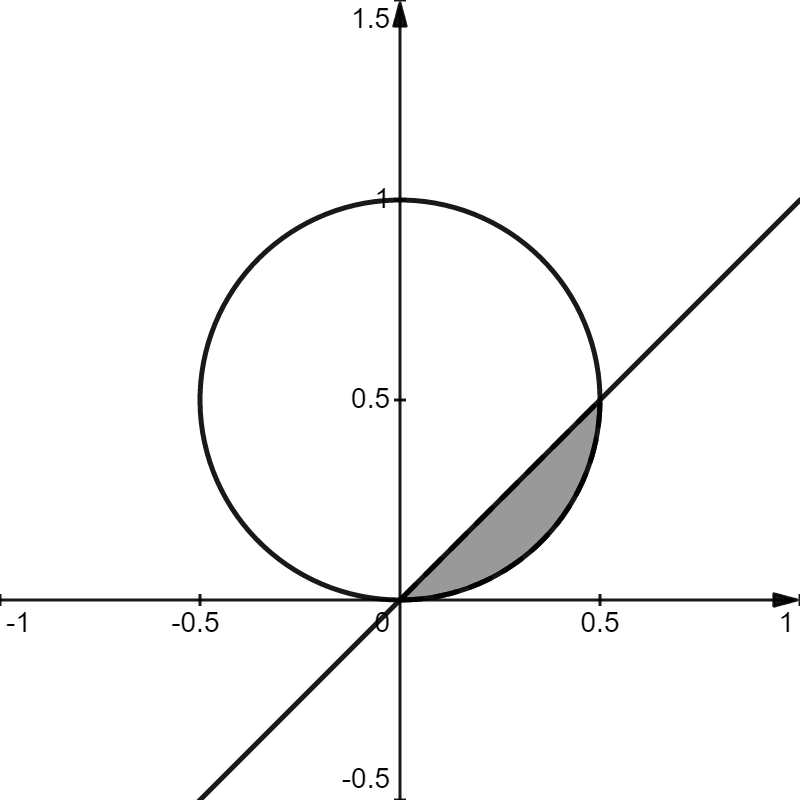
\includegraphics[width=50mm]{Images//ws7-sliver}\]

\item  Use a polar coordinates to find the volume of the solid region inside of the sphere $x^2+y^2+z^2=9$ and outside of the vertical cylinder $x^2+y^2=1$. 

\item  Describe the following surfaces in $3$-dimensional space
\begin{enumerate}
	\item $r^2+z^2=1$
	\item $r=2\cos \theta$
	\item $z=r \sin \theta$
	\item $z=r\sin \theta + 2r\cos \theta$
\end{enumerate}

\item A \textit{lemniscate} (i.e., figure eight) is a curve of the form $r^2=2a^2 \cos(2\theta)$ for some constant $a$ (as seen below with $a=1$). Use polar coordinates to find the area of the region inside the lemniscate, your answer will depend on $a$.

\[ 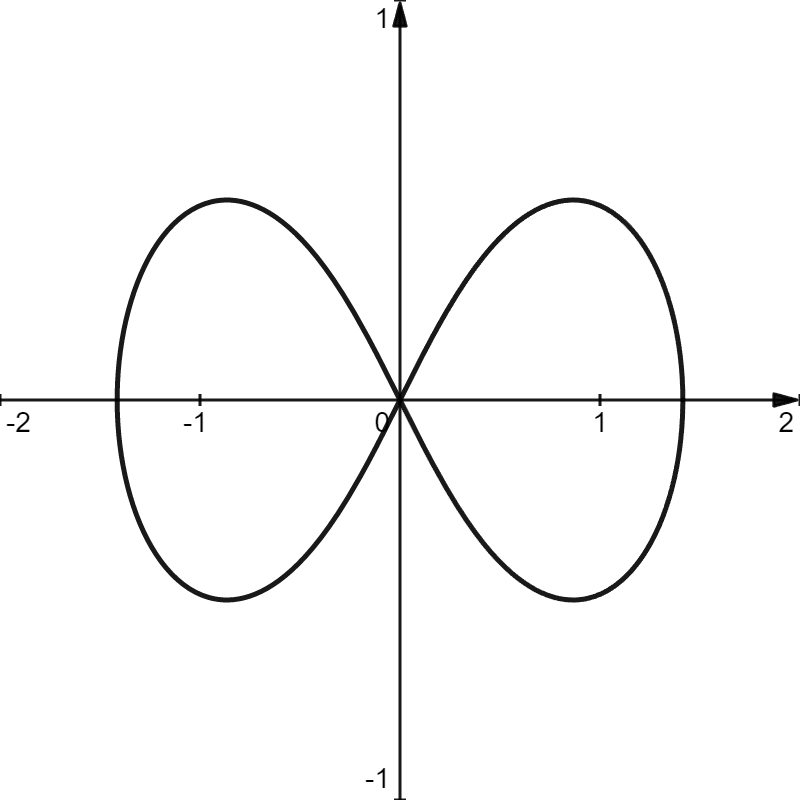
\includegraphics[width=60mm]{Images/ws7-lem}\]

\item \textit{True or False}. Determine if the following statements are true or false. Give a brief justification of your answer.

\textit{Suggestion}: If you want to test your understanding of polar coordinates, try to solve these using a geometric argument rather than just evaluating the integral.

\begin{enumerate}
	\item $\displaystyle \int_0^{2\pi} \int_0^1 1 \,dr\, d\theta=\pi$
	\item $\displaystyle \int_0^{\pi} \int_0^{\sin \theta} r \,dr \, d\theta=\pi/4$
	\item $\displaystyle \int_0^{2\pi} \int_0^1(3-r)r \,d{r}\,d\theta=\pi$
	\item $\displaystyle \int_0^{\pi/2} \int_0^{1/(\sin\theta+\cos\theta)}r \,d{r}\,d\theta=\dfrac{1}{2}$
\end{enumerate}

\end{enumerate}
Suggested additional exercises: \textit{Stewart} section 15.3







\section{**Change of coordinate systems}

Given a double integral $\iint_R f\,dA$ that you'd like to compute, it's often the case that either the function $f$ or the region $R$ is not reasonably integrated in the given $x,y$ coordinates. We've already seen polar coordinates; for triple integrals we'll learn similar strategies of \textit{cylindrical} and \textit{spherical} substitutions, but those are only some of the options. 

First, some basics: Suppose we have functions\footnote{These should be ``nice'', i.e., continuous, differentiable, etc.} $x=x(u,v)$ and $y=y(u,v)$, and want to evaluate a given definite \[\iint_R f\,dA\] by exchanging $x,y$ into the $u,v$ coordinate system. This is like doing a $u$-substitution in one variable calc, but also more complicated. The function $f$ can be turned into a function of $u,v$ by substituting in the given equations into the formula for $f$. But there's an additional factor by which the integral will change. It has to do with the \textit{Jacobian}. 

\subsection{The Jacobian}\label{jacobian-def}
Notationally, we write $\dfrac{\partial(x,y)}{\partial(u,v)}$ for the Jacobian. This factor is obtained from the determinant of the following matrix of partial derivatives
\begin{equation} J= \begin{pmatrix} x_u & x_v \\ y_u & y_v \end{pmatrix}\end{equation}
as follows: \begin{equation} \dfrac{\partial(x,y)}{\partial(u,v)} =|\det J|= |x_u y_v - x_v y_u|.\end{equation}

The bounds of the integral also need to be turned into $u,v$ coordinates. 

\begin{example} Let's say we want to integrate \[f(x,y)=\dfrac{x-y}{x+y}\] over the region $R$ bounded by: $x-y=0, x-y=1, x+y=1, x+y=3$. The region in $x,y$ and $u,v$ coordinates is given in Figure \ref{fig-change-of-var}.

\begin{figure}[h!]
\centering 
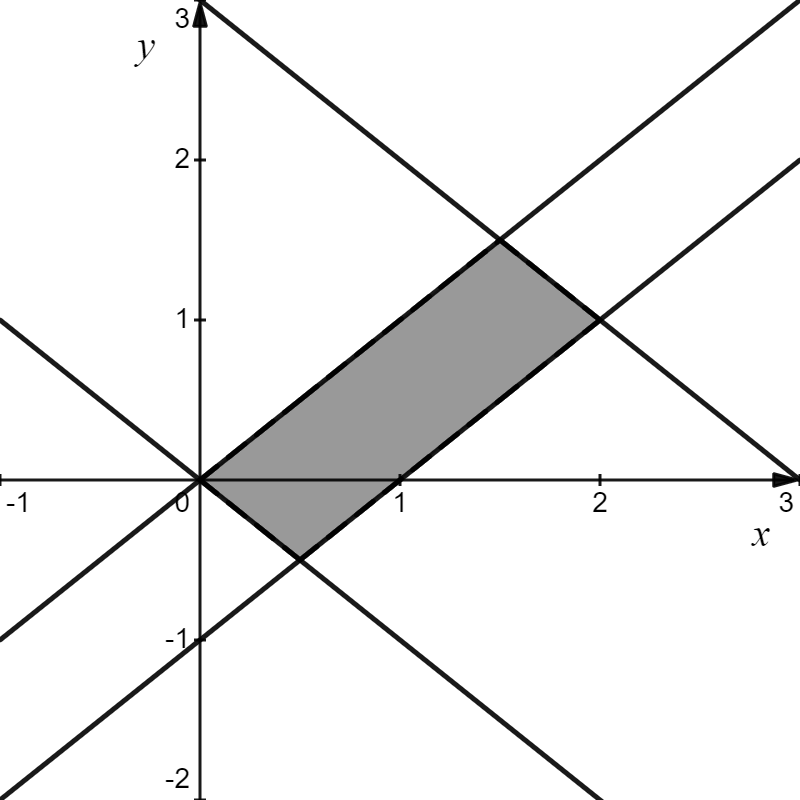
\includegraphics[height=50mm]{Images/ws65-xy} \hspace{30mm} 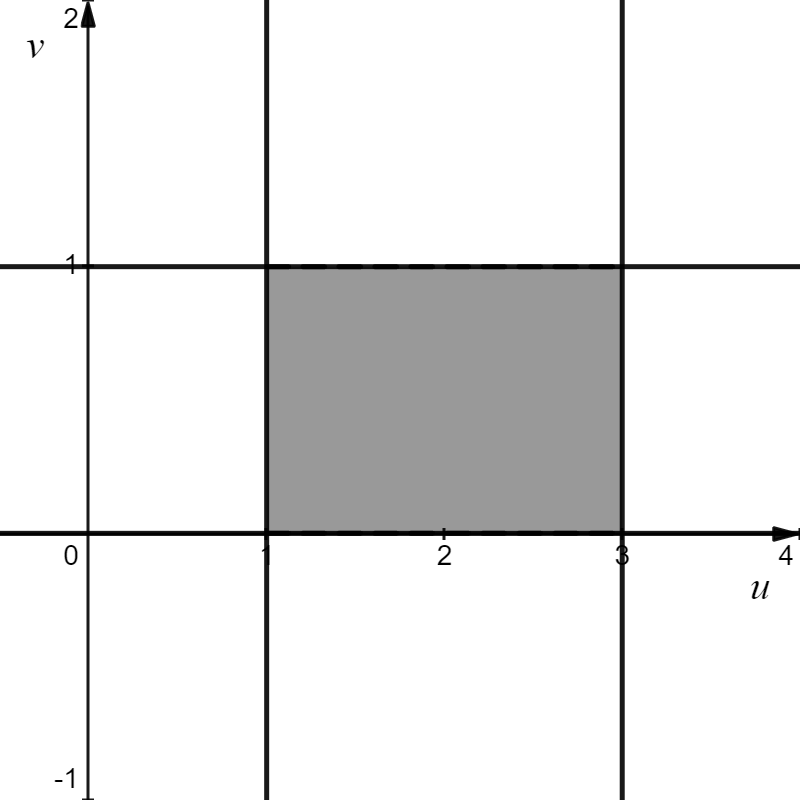
\includegraphics[height=50mm]{Images/ws65-uv}
\caption{Region $R$ in $xy$-coordinates (left), and corresponding $uv$-coordinates (right)}
\label{fig-change-of-var}
\end{figure}


With $x,y$ coordinates this is fairly tedious, as you'll need at least three separate integrals to evaluate it, but it's doable. However, a clever change of coordinate systems makes it much easier: Let's substitute $u=x+y$ and $v=x-y$. We can see that the new bounds of integration will be much nicer: $1\leq u\leq 3, 0\leq v \leq 1$. Solving for $x,y$ gives $x=(1/2)(u+v)$ and $y=(1/2)(u-v)$ so, 

\[ \dfrac{\partial(x,y)}{\partial(u,v)} = \left| \det \begin{pmatrix} 1/2 & 1/2 \\ 1/2 & -1/2 \end{pmatrix} \right|=|-1/4-1/4|=1/2\]

The integral $\iint_R f(x,y)\,dA$ can then  be evaluated

\[ \iint_R f(x,y)\,dA = \int_0^1 \int_0^3 \dfrac{v}{u} \dfrac{1}{2} \,dv\,du= \cdots = \dfrac{\ln 3}{4}.\] 
\end{example}

Cool. Of course this also works with three variables, where the matrix $J$ is replaced with the appropriate $3\times 3$ matrix of partials, and similarly for functions with more variables still. 

\subsection{Exercises}

\begin{enumerate}[label=\arabic*.]
\item Find the Jacobian $\dfrac{\partial(x,y)}{\partial(u,v)}$ for the following transformations

\begin{enumerate}
	\item $x=u+3v$, $y=3u-2v$
	\item $x=uv$, $y=u/v$
	\item $x=\sin(u)+\cos(v)$, $y=-\cos(u)+\sin(v)$
	\item $u=e^x, v=ye^{-x}$
\end{enumerate}

\item Use the transformation $u=x-2y$ and $v=2x+y$ to compute $\displaystyle \iint_R \dfrac{x-2y}{2x+y}\,dA$ where $R$ is the region bounded by $x-2y=1, x-2y=4, 2x+y=1$ and $2x+y=3$.

\item  Use the transformation $u=y/x$ and $v=xy$ to find $\displaystyle \iint_R xy^3\,dA$ where $R$ is the region bounded by $y=x, y=3x, xy=1$ and $xy=4$.

\item  Find a change of coordinate system $x=x(u,v)$ and $y=y(u,v)$ that sends the half-annulus bounded by circles $x^2+y^2=9$ and $x^2+y^2=1$ in the first and fourth quadrants in the $xy$-plane to the rectangle $1\leq u \leq 3, 0\leq v\leq 1$ in $u,v$ coordinates.
\end{enumerate}
Suggested additional exercises: \textit{Stewart} section 15.9

\section{Triple integrals}



A \textit{triple integral} is the evident analog of a double integral; the region of integration $R$ must be a solid region in $\mathbf{R}^3$ and the function $f$ to be integrated must be a three-variable function which has domain containing $R$. 

\subsection{Solid regions}
It's actually somewhat beyond the language of this class to give a definition of what a \textit{solid region}. but we can get close enough with the following: 

\begin{defn} \label{def-solid-region} A \textbf{solid region} in $\mathbf{R}^3$ is a 3 dimensional subset of $\mathbf{R}^3$ whose \textit{boundary} is a (finite) collection of surfaces.\end{defn}

By contrast, for double integrals we considered regions in $\mathbf{R}^2$ whose boundary consisted of a (finite) collection of curves. For instance, the box $0\leq x\leq 1, 0\leq y\leq 1, 0\leq z\leq 1$ is a solid region, but the \textit{surface} $x+y+z=1$ is not a solid region. We'll talk about how to integrate over surfaces in $\mathbf{R}^3$ later. 
Note that for our integrals to make sense, the solid regions $R$ we're considering must also be \textbf{bounded}\footnote{Like with two dimensional regions, it's sufficient here that $R$ be contained in some big enough sphere $x^2+y^2+z^2=r^2$, informally you can think of this as $R$ not ``going off to infinity" in any direction. Note that this is \textit{not} the same thing as requesting that $R$ have finite volume.}. 
	
	\begin{defn} Let $R$ be a solid region in $\mathbf{R}^3$ and $f$ a continuous function defined on $R$. The \textbf{triple integral} of $f$ over $R$ is the number \begin{equation} \iiint_R f\,dV\end{equation} given by ``continuous addition" of $f$ over $R$.
	\end{defn}
	
	\begin{remark}While one- and two-variable functions have definite integrals that can be interpreted as areas and volumes respectively, three (and more) variable functions lose the thread a bit. A triple integral \textit{could} be defined as  the $4$-dimensional ``hypervolume'' of the ``stuff'' between the graph $w=f(x,y,z)$ in $\mathbf{R}^4$ and the $xyz$-hyperplane. This is obviously hard to visualize, so it's better to just think of the triple integral $\iiint_R f\,dV$ as ``adding up'' the values of $f$ from the domain $R$ (for instance, $f$ could be density in which case $\iiint_R f\,dV$ is just the mass of this solid). \end{remark}

The differential $dV$ is the \textbf{volume differential} or \textbf{volume element}. As with double integrals, triple integrals are calculated by iterated integrals.
	
	
\subsection{Iterated integrals}
The first step here is to pick an order of integration; in $\mathbf{R}^3$ there are \textit{six}\footnote{$6=3!$, the number of ways to rearrange the three elements $dx$, $dy$ and $dz$. In $\mathbf{R}^n$ you have $n!$ different ways to set up an $n$-fold integral.} choices of orders of integration, meaning $dV$ is equal to any of the following: \[ dV=dx\,dy\,dz, \quad dy\,dx\,dz, \quad dx\,dz\,dy, \quad dz\,dx\,dy, \quad dy\,dz\,dx, \quad dz\,dy\,dx\]

Say we've decided that $dx\,dy\,dz$ is the order of integration we're going to use for a particular problem. Setting up a \textit{triple integral} amounts to finding the bounding functions for $R$  (you may need to split into several iterated integrals) so that \begin{equation} \iiint_R f\,dV = \int_a^b \int_{f(z)}^{g(z)}\int_{\alpha(y,z)}^{\beta(y,z)} f(x,y,z)\,dx\,dy\,dz\end{equation} Note how the bounds of the inner integrals only depends on variables from the outer integrals. 

\begin{remark} Most of the work here will be in finding these bounding functions for the region $R$, and a useful way to get started is to think of a triple integral as ``$2+1$''. That is, say you've decided that the inner variable of integration should be $z$, then the triple integral is set up as \[ \iiint_R f\,dV=\iint_{\text{projection of $R$ onto $xy$-plane}} \int_{\text{lower surface}}^{\text{upper surface}} f\,dz\,dA\] \end{remark}


Actually evaluating triple integrals is really just evaluating three integral (remember: iterated integrals always are evaluated inside to out). It's no secret getting a numerical answer can often be somewhat tedious. 
	
\subsection{Integrals with more variables} 
	 Similarly, there's nothing from stopping you from integrating functions of more variables. If $f=f(x_1,\dots,x_n)$ is a function of $n$ variables and $R$ is some ($(n+1)$-dimensional) region in $\mathbf{R}^n$, you can just as well define \begin{equation} \int \cdots \int_R f\,d\mathcal{V}\end{equation} where $d\mathcal{V}$ is the ``$n$-dimensional hypervolume element'', i.e.,  just means some order of the elements $dx_1, \dots dx_n$. It's up to you to determine how this will be useful. 


\subsection{Exercises}
\begin{enumerate}[label=\arabic*.]
\item Evaluate the following triple integrals

\begin{enumerate}
	\item $\displaystyle \int_0^1 \int_0^1 \int_0^3 (xy+yz+x^2) \,dx\,dy\,dz$
	\item $\displaystyle \int_0^1 \int_1^y \int_y^{x^2} 2y \,dz\,dx\,dy$
	\item $\displaystyle \int_{-1}^1 \int_z^1 \int_0^{y} \dfrac{y}{x^2+y^2} \,dx\,dy\,dz$
\end{enumerate}

\item Evaluate the following triple integrals over the given region $R$ by setting up a system of iterated integrals

\begin{enumerate}
	\item $\displaystyle \iiint_R xy \sin(z)\,dV$ \quad $R$ is the box defined by $0\leq x \leq 1, 0\leq y \leq 2, 0 \leq z \leq \pi/2$
	\item $\displaystyle \iiint_R x \,dV$ \quad  \quad $R$ the solid enclosed by $z=x$ and $x=1-y^2$ above the $xy$-plane
	\item $\displaystyle \iiint_R (x+y+z)\,dV$ \quad $R$ the solid enclosed by $x^2+y^2+z^2=1$ in the first octant
	\item $\displaystyle \iiint_R (2y-z)\,dV$ \quad $R$ the solid enclosed by paraboloids $z=1-x^2-y^2$ and $z=x^2+y^2-1$.
\end{enumerate}

\item Let $f=f(x,y,z)$ be some continuous function defined on the given region. Rewrite the following integrals to be of the form $\iiint f(x,y,z)\,dz\,dy\,dx$

\begin{enumerate}
	\item $\displaystyle \int_0^1 \int_0^{1-\sqrt{x}} \int_0^z f(x,y,z) \,dy\,dz\,dx$
	\item $\displaystyle \int_0^{16} \int_0^2 \int_0^{x/2} f(x,y,z) \,dy\,dz\,dx$
	\item $\displaystyle \int_0^1 \int_0^2 \int_0^{\sqrt{4-y^2}}f(x,y,z)\,dx\,dy\,dz$
\end{enumerate}

\item The \textit{average value} of a continuous function $f$ defined on a region $R$ in 3 dimensional space is given by \[ \bar{f}= \dfrac{1}{\text{volume of $R$}} \iiint_R f\,dV.\]

Find the average value of $f(x,y,z)=x+y+z$ defined on the tetrahedron with vertices at $(0,0,0)$, $(1,0,0), (0,1,0)$ and $(0,0,1)$.

\item Find the average value of $f(x,y,z)=xyz$ defined on the solid sphere $x^2+y^2+z^2\leq 1$ (\textit{hint: can you guess what it should be?})

\item Set up a triple integral which computes the volume of the piece of the solid cylinder $y^2+z^2\leq 1$ cut by the planes $y=x$ and $x=0$ in the first octant. 
\end{enumerate}

Suggested additional exercises: \textit{Stewart} sections 15.6

\section[Cylindrical and spherical coordinates]{Triple integrals in cylindrical and spherical coordinates}

Here we consider two commonly used substitutions for triple integrals: cylindrical and spherical coordinates.

\subsection{Cylindrical coordinates}
Cylindrical coordinates are really not all that new: most of the work behind them we already know from polar coordinates. The idea is to replace two of the three variables $x,y,z$ with their polar analogues. For simplicity, let's say we've made the substitutions \[ x=r\cos \theta, y=r\sin \theta\] and left $z$ alone. Then we could write: \begin{equation} \label{cyl-sub} dV=dz \,dx\,dy=dz\, dA=r \,dz \,dr\,d\theta\end{equation} 
where the last step comes from the differential $dA=r \,dr\,d\theta$ for polar coordinates. It's often best to have the unsubstituted variable on the inner most integral, so that you can define its bounds in terms of $r$ and $\theta$. Remember, the idea here is that the polar substitution on your variables should be \textit{helpful}!

\subsection{Cylindrical coordinate substitution in triple integrals} For a function $f=f(x,y,z)$ defined and continuous on a region $R$, \begin{equation}\iiint_R f\,dV=\iiint_{\text{$R$ in cylindrical coord.}} f(r\cos\theta,r\sin\theta,z)\, r \,dz  \,dr \, d\theta \end{equation}

\begin{remark}
	Of note is that this is just \textit{one} type of cylindrical substitution. While we think of the cylindrical substitution as replacing variables $x,y$ in terms of $r,\theta$; it's not strictly necessary that those be the substituted variables. This first type of substitution is useful when the region $R$ is symmetric (radially) about the $z$-axis of $\mathbf{R}^3$. However \[x=x,\quad y=r\cos\theta,\quad  z=r\sin\theta\] is another valid cylindrical substitution. This latter type could be useful for a region $R$ which is symmetric about the $x$-axis. In all, there are three (or six, depending on how you think about it) different cylindrical substitutions. However, they all operate more or less the same.
\end{remark}


\subsection{Spherical coordinates}
Spherical coordinates are something new to working with triple integrals. The idea here is to describe a point $P=(x,y,z)$ in $\mathbf{R}^3$ in terms of the following information 
\begin{itemize}
	\item The distance $\rho$\footnote{$\rho$ is the Greek letter \textit{rho}---it makes the [r] sound in English. Please note, this is not the letter ``p''} to the origin 
	\item Angles $\theta$ and $\varphi$\footnote{$\varphi$ is the Greek letter \textit{phi}---it makes the [f] sound in English} which tell you location on the unit sphere $x^2+y^2+z^2=1$ in $\mathbf{R}^3$.
	
	
\end{itemize}

We need to define these coordinates $\theta$ and $\varphi$. The angle $\theta$ is the same as in polar coordinates, the angle from the positive $x$-axis (in the $xy$-plane) measures counter-clockwise. Angle $\varphi$ gives the angle \textit{downward} (toward the $xy$-plane) from the positive $z$-axis to the point $P$ (see Figure \ref{fig-spherical})\footnote{A small annoyance that you may encounter (particular in the field of \textit{electrical engineering} is that the roles of $\varphi$ and $\theta$ are flipped form what we're about to write here. This makes little sense to me, $\theta$ should be the same $\theta$ as with polar coordinates, just be aware of it.}. 

\begin{figure}[h!]
\centering 
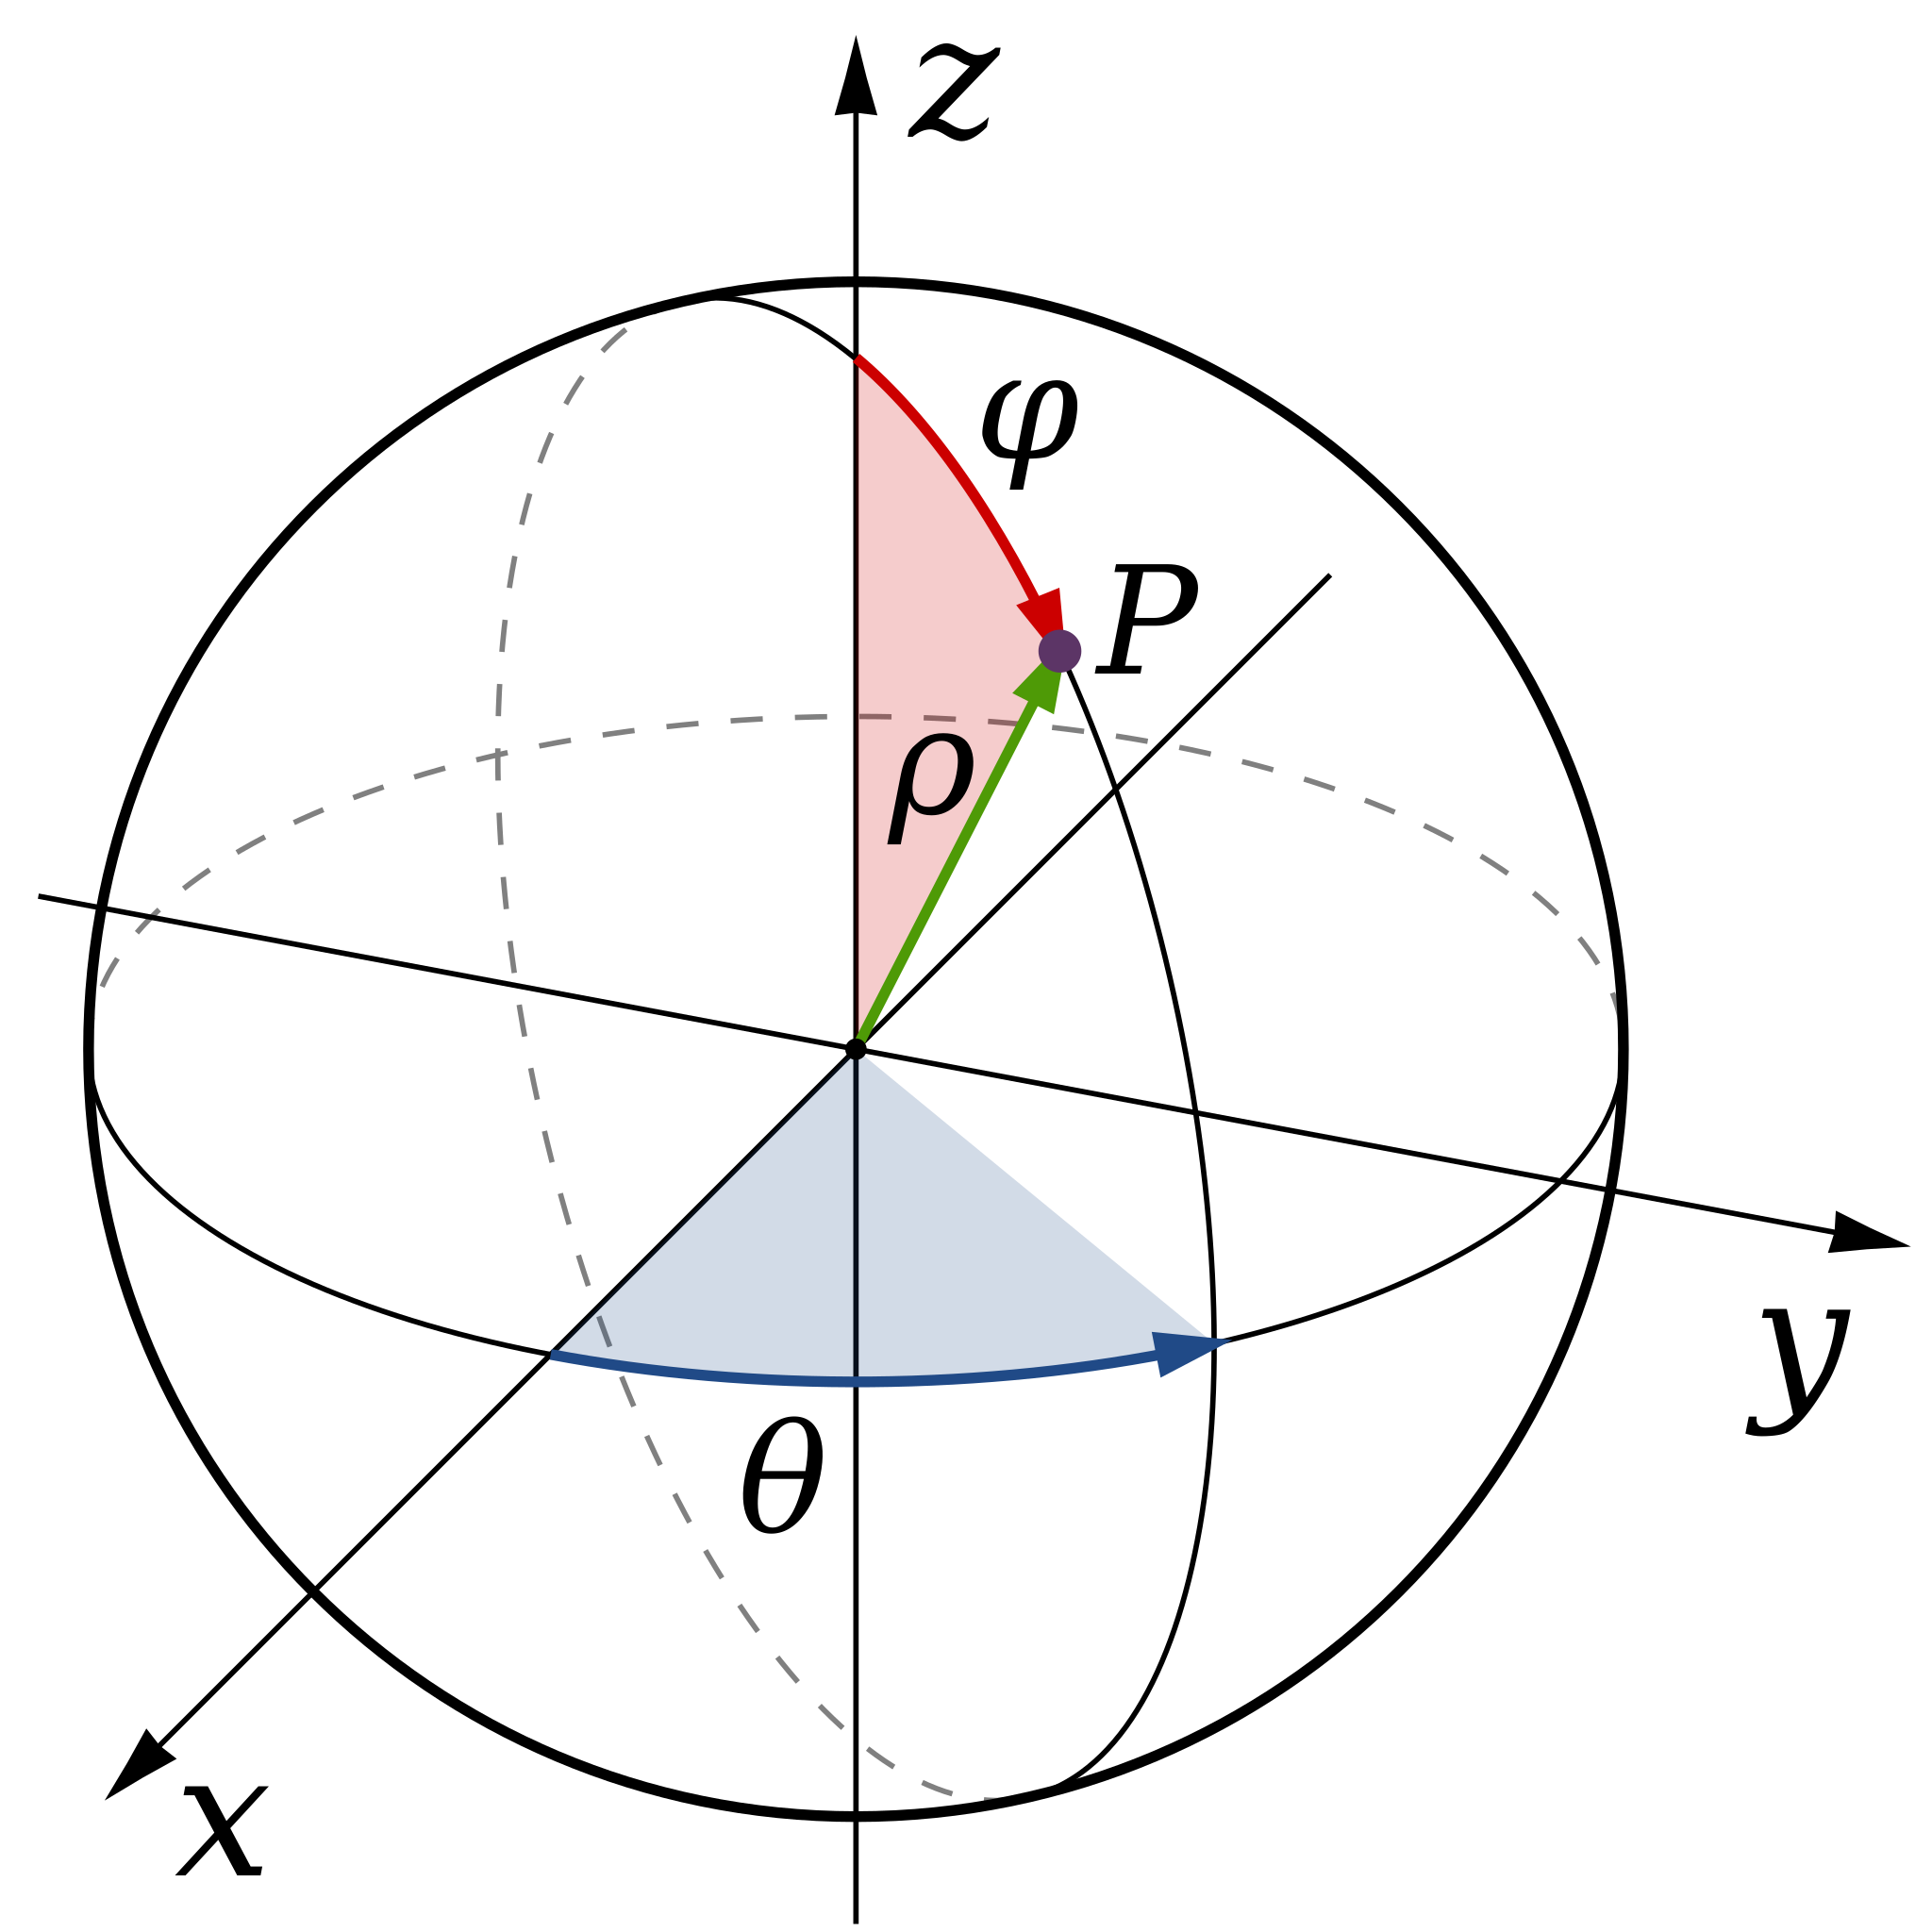
\includegraphics[width=60mm]{Images/ws9-spherical} 
\caption{Spherical coordinates}
\label{fig-spherical}
\end{figure}

It's a nice exercise to convince yourself that the domain of $0\leq \theta\leq 2\pi$ and $0\leq \varphi \leq \pi$ is enough to cover the unit sphere \textit{once}. We then get the \textbf{spherical coordinate substitutions}
\begin{equation} 
	x=\rho \cos \theta \sin \varphi, \qquad y=\rho \sin \theta \sin \varphi, \qquad z=\rho \cos \varphi \label{spherical-coord}
\end{equation}
It's another nice exercise to check that $x^2+y^2+z^2=\rho^2$ (\textit{can you find equations for $\theta$ and $\varphi$ in terms of $x,y,z$? it's possible but not exactly easy}) Lastly, we need to compute the differential $dV$ in terms of spherical coordinates. The same \textbf{Jacobian determinant} (see \ref{jacobian-def}) shows up here, which I leave for you to check: \[ \det \begin{pmatrix} x_{\rho} & x_{\theta} & x_{\varphi} \\ y_{\rho} & y_{\theta} & y_{\varphi} \\ z_{\rho} & z_{\theta} & z_{\varphi} \end{pmatrix} =\rho^2\sin\varphi\] 


Since the term $\rho^2\sin\varphi$ is always $\geq 0$ for $\varphi$ in the interval $[0,\pi]$, we get that \begin{equation} dV= \rho^2 \sin\varphi \, d\rho \,d\varphi\, d\theta \label{dV-spherical} \end{equation}

\subsection{Spherical coordinate substitution in triple integrals} Putting it all together, we get the spherical coordinate substitution: For a function $f=f(x,y,z)$ defined and continuous on a region $R$, \begin{equation}\iiint_R f\,dV=\iiint_{\text{$R$ in spherical coord.}} f(\rho\cos\theta\sin\varphi, \rho\sin\theta\sin\varphi, \rho\cos\varphi)\, \rho^2 \sin\varphi \,d\rho\,d\varphi \, d\theta \end{equation}

\begin{remark}
As with polar substitutions, the order $d\rho\, d\varphi\, d\theta$ is more or less fixed by virtue of how these variables are defined. That is, it's often easiest/only possible to describe $\rho$ in terms of $\theta, \varphi$ and $\varphi$ in terms of $\theta$. For instance, $\rho=\sec\varphi$ is the spherical function which defines the plane $z=1$.

 \end{remark}

While this may seem like a lot of information, the goal here is to use these substitutions to \textit{simplify} what it is we are calculating: this often means getting to avoid many cumbersome trig-substitution integral calculations.

\subsection{Exercises}
\begin{enumerate}[label=\arabic*.]
\item Evaluate the following triple integrals. If possible, describe the region of integration in the $xyz$-space in terms of cylindrical or spherical coordinates.

\begin{enumerate}
	\item $\displaystyle \int_0^{\pi} \int_0^{\cos \theta} \int_0^{r^2} r\sin \theta \,dz  \,dr\, d\theta$
	\item $\displaystyle \int_0^{2\pi} \int_{0}^{\pi/4} \int_0^{\sec \theta}  \rho^3 \sin \varphi \,d \rho\,d\varphi\,d\theta$
\end{enumerate}

\item Use spherical coordinates to find the following volumes

\begin{enumerate}
	\item The volume of the solid bounded above by the sphere $\rho=4$ and below by the cone $\varphi=\pi/3$. 
	\item The solid inside the sphere $x^2+y^2+z^2=16$ between planes $z=1$ and $z=3$
	\item The solid inside the sphere $x^2+y^2+z^2=1$ outside the cone $\varphi=\pi/4$ in the first octant
\end{enumerate}

\item  Use cylindrical coordinates to find the volume of the solid enclosed by the paraboloid $z=x^2+y^2$ and the plane $z=9$. 

\item Evaluate the following integrals by using either spherical or cylindrical coordinate substitution

\begin{enumerate}
	\item $\displaystyle \int_{-1}^{1} \int_0^{\sqrt{1-x^2}} \int_0^{\sqrt{1-x^2-y^2}}e^{-(x^2+y^2+z^2)^{3/2}} \,dz \,dy \, dx$
	\item $\displaystyle \int_{0}^{2} \int_0^{\sqrt{4-x^2}} \int_{\sqrt{x^2+y^2}}^{\sqrt{8-x^2-y^2}} z^2 \,dz \,dy \, dx$
\end{enumerate}

\item Describe the given by the following equations of spherical coordinates

\begin{enumerate}
	\item $\varphi=\frac{\pi}{3}$
	\item $\rho=1$
	\item $\theta=\pi$
	\item $1=\rho \cos \varphi$
	\item *$1=\rho \cos \varphi - \rho^2 \sin^2 \varphi$

\end{enumerate}

\item Evaluate $\iiint_R xyz \,dV$ where $R$ is the region inside the sphere $x^2+y^2+z^2=1$ in the first octant using (i) Cartesian coordinates, (ii) cylindrical coordinates, (iii) spherical coordinates. Which one is easiest?

\item Use cylindrical coordinates to derive the volume of a cone of radius $s$ and height $h$ (\textit{hint: Find the volume of the region between $z=h$ and $z=(h/s)r$}).

\item Show that the following formula for the Jacobian determinant of the spherical coordinate substitution is indeed correct \[ \det \left( \begin{matrix} x_{\rho} & x_{\varphi} & x_{\theta} \\ y_{\rho} & y_{\varphi} & y_{\theta} \\ z_{\rho} & z_{\varphi} & z_{\theta} \end{matrix} \right)= \rho^2 \sin \varphi \]
and moreover that for spherical coordinates substitutions $x^2+y^2+z^2=\rho^2$.

\item *In this problem we'll compute the ``hyper-volume'' enclosed by the 3-dimensional sphere $S^3$. Note that the $1$-dimensional sphere $S^1$ is the usual unit circle $x^2+y^2=1$ in the $xy$-plane. Similarly, the $2$-dimensional sphere $S^2$ is given by the equation $x^2+y^2+z^2=1$ in $xyz$-space. We know $S^1$ encloses an area of $\pi$ ($\pi r^2$ with $r=1$) and $S^2$ encloses a volume of $\frac{4}{3}\pi$ ($\frac{4}{3}\pi r^3$ with $r=1$). 

The three-dimensional sphere $S^3$ is given by the equation $x^2+y^2+z^2+w^2=1$ in the 4-dimensional $xyzw$-hyperspace (that is, just $\mathbf{R}^4$ with coordinates given by quadruples $(x,y,z,w)$). We will make a substitution into ``hyper-spherical'' coordinates $(r,\theta, \varphi, \psi)$, given by:
\[x=r \cos\theta \sin \varphi \sin \psi, \; y=r \sin \theta \sin \varphi \sin \psi , \; z=r \cos \varphi\sin \psi , \; w=r\cos \psi\]

\begin{enumerate}
	\item Compute the determinant of the $4\times 4$ Jacobian matrix given by 
	\[ J=\begin{pmatrix} x_r & x_{\theta} & x_{\varphi} & x_{\psi} \\
	y_r & y_{\theta} & y_{\varphi} & y_{\psi}\\
	z_r & z_{\theta} & z_{\varphi} & z_{\psi}\\
	w_r & w_{\theta} & w_{\varphi} & w_{\psi}
	\end{pmatrix}\]
	to show that \[d\mathcal{V}= r^3 \sin \varphi  \sin^{2}\psi \, dr\, d\theta \, d\varphi \, d\psi\] (here, $d\mathcal{V}$ is the differential for ``hypervolume'').
	\item The unit $3$-dimensional sphere in $xyzw$-hyperspace is given by bounds: \[0\leq r \leq 1, \quad  0\leq \theta \leq 2\pi, \quad 0\leq \varphi \leq \pi, \quad 0\leq \psi \leq \pi.\] Use this to set up a in integral in hyperspherical coordinates which evaluates the following 
	\[ \iiiint_{\text{stuff inside $S^3$}} 1\, d\mathcal{V}\] 
	\item Evaluate the integral from part b. to show that the hypervolume enclosed by the unit 3-sphere $S^3$ given by equation $x^2+y^2+z^2+w^2=1$ is $\frac{1}{2}\pi^2$. (Note, in general the $3$-dimensional sphere of radius $r$ will enclose a region of hypervolume $\frac{1}{2}\pi^2 r^4$.)
	%\item Let $V_n$ denote the ``$(n+1)$-dimensional hypervolume'' enclosed by the $n$-dimensional sphere $S^n$ in $(n+1)$-dimensional space. Use the recurrence relation $V_{n}=2\pi V_{n-2}/n$ to show that the $(n+1)$-dimensional hypervolume enclosed by the $n$-dimensional sphere goes to $0$ as $n\to \infty$.
\end{enumerate}
\end{enumerate}
Suggested additional exercises: \textit{Stewart} sections 15.7, 15.8




\section{Centroids and centers of mass}

Let's consider the following problem: for a region $R$ in $\mathbf{R}^2$, what is the \textit{center} of $R$? if $R$ is a disc, e.g. $x^2+y^2=1$ we know that the center is the center of the disc, in this case the origin (what other shapes do we ``know'' the center of already?). 

In general, the ``center'' of a shape is called the \textbf{centroid}. If you think of $R$ as a very thin sheet of some material of uniform density, the centroid would be the point of balance\footnote{This makes sense for 2D-regions here, as you could imagine balancing this thin sheet of material on your finger, but won't quite line up with our intuition from interacting with the ``real world" when talking about centroids for 3D-regions.} for $R$. 

\begin{defn}[Centroid]Let $R$ be a region in $\mathbf{R}^2$. The \textbf{centroid} of $R$ is the point $(\bar{x},\bar{y})$ computed via \begin{equation}
	\label{centroid} \bar{x} =\dfrac{\iint_R x\,dA}{\iint_R 1\,dA} \qquad \qquad \bar{y} =\dfrac{\iint_R y\,dA}{\iint_R 1\,dA}
\end{equation} \label{centroid-def-2}
\end{defn}
\begin{remark}Note that $\iint_R 1\,dA$ is just the \textit{area} of the region $R$, what then are the numerators for the coordinates $\bar{x}$ and $\bar{y}$? We can think of $\iint_R x\,dA$ as ``adding up'' all the $x$ values of $R$ (resp. with $y$), so really $\bar{x}$ and $\bar{y}$ are just the \textit{average} $x$ and $y$ coordinates of $R$. Thought of this way, the ``center'' (centroid) of the region is just what you get by the average of the $x$ and $y$ coordinates of that region. \end{remark}

\subsection{Center of mass}
One neat modification of this idea leads us to the \textbf{center of mass} of a region $R$. Let's define a \textbf{density function} to be a continuous function $\delta\colon R\to [0,\infty)$\footnote{Density in terms of mass density should probably be positive, though it could be useful to talk about something like density of electric charge in which case you'd change the range accordingly.} where $R$ is some region in $\mathbf{R}^2$. Given a region $R$ and density function $\delta$, the expression \begin{equation} \iint_R \delta \,dA\end{equation} is the \textbf{total mass} of $R$ (with respect to the density $\delta$).

\begin{defn}[Center of mass]Let $R$ be a region in $\mathbf{R}^2$ and $\delta$ be a density function on $R$. The \textbf{center of mass} of $R$ is the point $(m_x,m_y)$ computed as \begin{equation}
	\label{com} m_x =\dfrac{\displaystyle \iint_R x \delta(x,y) \,dA}{\displaystyle \iint_R \delta(x,y)\,dA} \qquad \qquad m_y =\dfrac{\displaystyle \iint_R y \delta(x,y) \,dA}{\displaystyle \iint_R \delta(x,y)\,dA}
\end{equation}\label{com-def-2}
\end{defn}
Similar to \eqref{centroid} we can think of the center of mass as a \textit{weighted} average of the $x$ and $y$ coordinates of $R$. 

\begin{remark}One good mathematical interpretation is when $\delta$ is a probability density function (i.e., $\iint_R \delta\,dA=1$), in which case the center of mass is just the \textit{expected value} of the random variable represented by $\delta$\footnote{That is, the random variable $X$ such that for  $D\subset R$ \[P(X\in D)= \iint_D \delta \,dA\]}. \end{remark}

\subsection{Centroids and center of mass in $\mathbf{R}^3$}
The evident analogs of \textit{centroid} and \textit{center of mass} from definitions \ref{centroid-def-2} and \ref{com-def-2} are what you'd probably expect for a solid region $R$ in $\mathbf{R}^3$. That is, the centroid is the point $(\bar{x},\bar{y},\bar{z})$ with coordinates computed as \begin{equation} \bar{x} =\dfrac{\iiint_R x\,dV}{\iiint_R 1\,dV}, \quad \bar{y} =\dfrac{\iiint_R y\,dV}{\iiint_R 1\,dV}, \qquad \bar{z} =\dfrac{\iiint_R z\,dV}{\iiint_R 1\,dV} \end{equation}
with the appropriate change for the center of mass formulas as well. 

\subsection{Exercises}
\begin{enumerate}[label=\arabic*.]
\item Find the coordinates of the centroid for the following regions $R$

\begin{enumerate}
	\item $R$ the triangle in the $xy$-plane with vertices $(0,0), (0,4), (3,0)$ 
	\item $R$ the portion of the disc $x^2+y^2=9$ within the first quadrant
	\item $R$ the unit square in the first quadrant
	\item $R$ the region bound by $y=1/x, y=-1/x$ and the lines $y=\pm 2, x=\pm 2$
\end{enumerate}
\item  Find the center of mass for the unit square in the first quadrant of the $xy$-plane with density function $\delta(x,y)=xy$. Do the same for the unit circle in the $xy$-plane with $\delta(x,y)=x^2+y^3$

\item  Show that the integrals which compute the center of mass $(\bar{x},\bar{y})$ of a region $R$ in polar coordinates are
 \[ \bar{x}=\dfrac{1}{\text{area of $R$}} \iint_R r^2 \cos(\theta) \,d{r}\,d\theta \qquad \bar{y}=\dfrac{1}{\text{area of $R$}} \iint_R r^2 \sin(\theta) \,d{r}\,d\theta\]
 
 \item  Show that if $R$ is a triangle with vertices $(a_1,b_1), (a_2,b_2), (a_3,b_3)$, then the centroid of $R$ is given by \begin{equation} \bar{x} =\dfrac{a_1+a_2+a_3}{3}\qquad \qquad \bar{y} = \dfrac{b_1+b_2+b_3}{3}\end{equation}

Show as well that the centroid of a triangle is equal to its \textbf{barycenter}\footnote{If you may have ``forgotten'', the barycenter of a triangle is the intersection the three lines connecting the midpoint of a leg to the opposite vertex of the triangle (see Figure \ref{fig-barycenter})}

\begin{figure}[h!] \centering
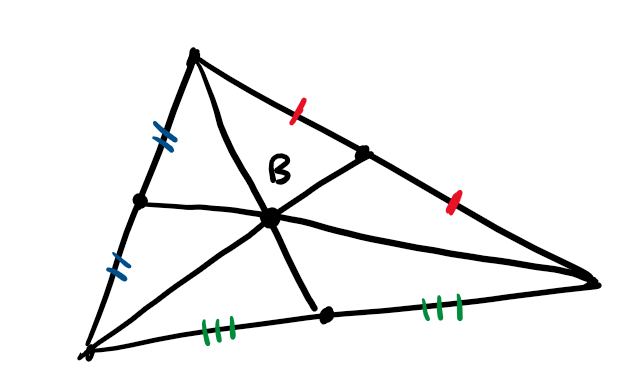
\includegraphics[width=70mm]{Images/barycenter}
\caption{A construction of the barycenter $B$ of a triangle}
\label{fig-barycenter}
\end{figure}

\item The \textit{moment of inertia} of a solid is its tendency to resist rotation about a particular axis. The moments of inertia $I_x,I_y,I_z$ with respect to the coordinate axes of a solid $R$ in the $xyz$-space with constant density $\delta=1$ are given by: \[ I_x = \iiint_R (y^2+z^2)\,dV, \quad I_y = \iiint_R (x^2+z^2)\,dV, \quad  I_z = \iiint_R (x^2+y^2)\,dV\]

Find the moment of inertia $I_z$ for $R$ the solid cylinder $x^2+y^2\leq 1$ with $0\leq z\leq 2$. Then, compute $I_x$ for $R$ the solid sphere $x^2+y^2+z^2\leq 4$ in the first octant, and argue why $I_x=I_y=I_z$ for this second region. 

\item  Let $\delta$ be given by \[\delta(x,y)=\dfrac{1}{2\pi} e^{-(x^2+y^2)/2}\] This function has $\iint_{\mathbf{R}^2} \delta\,dA=1$\footnote{One way to show this is by polar substitution: \[ \iint_{\mathbf{R}^2} \dfrac{1}{2\pi} e^{-(x^2+y^2)/2}\,dA=\int_{0}^{2\pi} \int_0^{\infty} \dfrac{r}{2\pi} e^{-r^2/2}\,dr\,d\theta= \left.2\pi \cdot \dfrac{1}{2\pi}e^{-u} \right\vert_{0}^{\infty}=1\] (Yes you ``should" use limits to evaluate the improper integral.)}, so we can interpret the center of mass $(m_x,m_y)$ as the expected value (i.e., average) of a probability distribution (This $\delta$ is just the two variable \href{https://en.wikipedia.org/wiki/Normal_distribution}{standard normal distribution}). Show that the expected value is $(0,0)$.

\item  \textit{True or False}. Determine if the following statements are true or false. Give a brief justification of your answer

\begin{enumerate}
	\item If a region $R$ is contained in the first quadrant, then all coordinates of its centroid will be nonnegative. 
	\item If a region $R$ has centroid $(0,0)$ then $R$ must be a disc
	\item Let $R$ be a region of the $xy$-plane with density function $\delta(x,y)=k$, $k$ some constant. Then its centroid and center of mass will always be the same
	\item If $R$ is a region in the $xy$-plane, and $\delta$ a  nonconstant density, then the centroid and center of mass of $R$ must be different points

\end{enumerate}
\end{enumerate}
Suggested additional exercises: \textit{Stewart} section 15.4



\section{Vector fields} \label{sec-vector-field}

With the basics of multivariable differential and integral calculus under our belt, the remainder of this course is dedicated to the field of \textbf{vector calculus}. To put it in perspective, so far we've dealt with the following:
\begin{itemize}
	\item Parametrized curves: functions $r\colon \mathbf{R}\to \mathbf{R}^n$, $n\geq 2$
	\item Multivariable functions: functions $f\colon \mathbf{R}^n\to \mathbf{R}$, $n\geq 2$
\end{itemize} and and worked with how to understand graphically what they represent. Now we move to a new type of function of multiple variables, called \textit{vector fields}. Vector fields have many uses throughout math, science and engineering; perhaps the most immediately useful is that vector field are \textit{the things} which carry forces in physics\footnote{In the classical (i.e., non-quantum) sense at least. There are also \textit{Quantum field theories} but this is a much more advanced topic.} (for instance, gravitational fields, electromagnetic fields, etc.).

\begin{defn}[Vector field]Let $n\geq 2$. A \textbf{vector field} $F$ on $\mathbf{R}^n$ is given by a function \[F\colon \mathbf{R}^n\to\mathbf{R}^n.\] In words, we say that ``$F$ is a vector field on $\R^n$" to mean that $F$ is a function $\R^n\to\R^n$.
\end{defn}


Graphically, a vector field $F$ is collection of vectors\footnote{Consider it like a field of wheat blowing in the wind; each stalk is the vector at that point.} one for each point in  $\mathbf{R}^n$. Vector fields are \textit{continuous} or \textit{differentiable} if this choice of vector depends \textit{continuously} or \textit{differentiably} on the points in $\mathbf{R}^n$ that produce them: this is a routine calculation to verify, but often no visually obvious. One of our goals is to determine ``visual cues'' for differentiability of vector fields. 

\begin{example} If $F$ is a vector field on $\mathbf{R}^2$. Then, $F$ is made up of \textit{component functions} $f,g$ (both functions of two variables) such that \begin{equation}F(x,y)=(f(x,y),g(x,y)).\end{equation} Then, given a point $(x,y)$ we think of the output $F(x,y)$ as the vector $(f(x,y),g(x,y))$ plotted in $\mathbf{R}^2$ with its tail at $(x,y)$\footnote{Recall that though ``all vectors start at the origin" it is often useful to blatantly ignore this advice, this is one of those times.}.

\label{Ex-vf-R2} Some examples of vector fields in $\mathbf{R}^2$ are in Figure \ref{fig-ex-vf}.
\begin{figure}[h!] \centering 
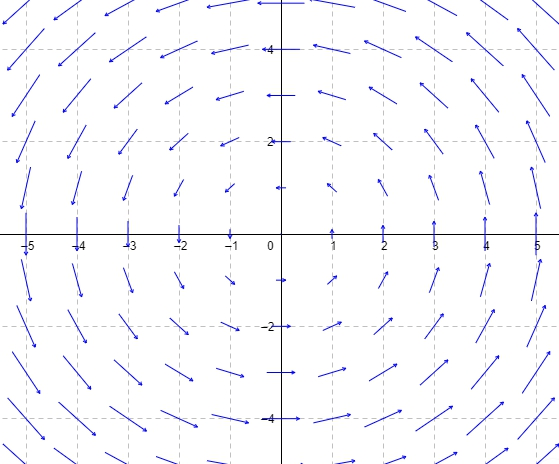
\includegraphics[width=50mm]{Images/ws21-a} 
\quad 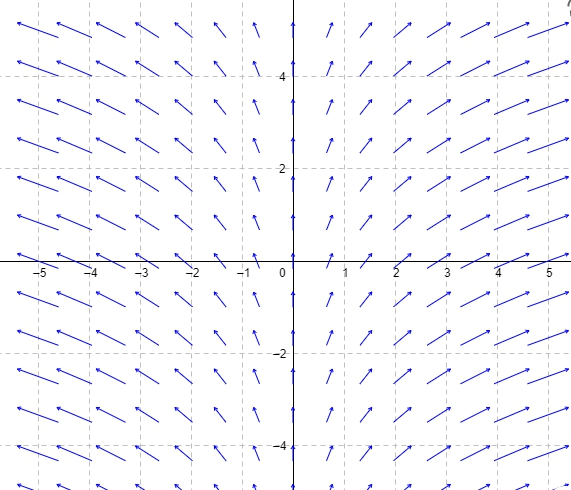
\includegraphics[width=50mm]{Images/ws21-b}
\quad 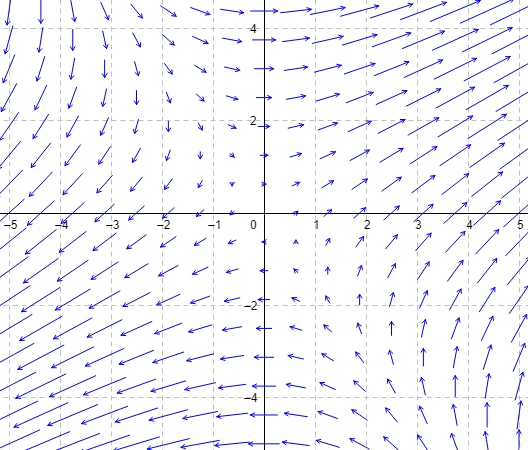
\includegraphics[width=50mm]{Images/ws21-d} 
\caption{Some vector fields on $\R^2$}
\label{fig-ex-vf}
\end{figure}
\end{example}

\begin{remark}In general, it's often quite difficult to produce a reasonably useful plot of a given vector field. As far as software goes, \href{https://www.math3d.org/}{Math3D} has a great tool for plotting vector fields in $\mathbf{R}^2$ and $\mathbf{R}^3$, but you'll probably need to finagle the parameters a bit to make the picture ``understandable''. There's also a (somewhat) useful \href{https://www.geogebra.org/m/QPE4PaDZ}{Geogebra applet} but Geogebra can be very hit or miss in terms of usability. 

Wolfram Mathematica is also quite good at plotting vector fields (and many other useful pictures), but is not free and has an interface which feels more like coding than Math3D or Geogebra. If this doesn't daunt you, you can get a license through the tech support office.  \end{remark}

\subsection{The gradient vector field}
We already know of a good wealth of examples of vector fields---specifically those from the gradient. 

\begin{fact} Let $f$ be a multivariable function $\mathbf{R}^n\to \mathbf{R}$. Then $\nabla f$ is a vector field on $\mathbf{R}^n$. 
\end{fact}

For instance, the function $f(x,y)=xe^y$ has the gradient vector field $\nabla f (x,y)=(e^y, xe^y)$. 

\begin{remark}[Gradient vector field is ``the derivative" of a multivariable function]We'll see soon that not all vector fields are gradient vector fields, and learn of special properties of those which are. An informal take is that $\nabla f$ is ``the thing'' which should be ``the derivative'' of $f$, however, when $f$ is a function of $2$ or more variables, this is telling us that ``the derivative'' of $f$ is no longer the same type of function. This story will be built upon throughout the remainder of this term, and is one of the reasons why vector calculus is so interesting/difficult.\end{remark}

\subsection{Exercises}

\begin{enumerate}[label=\arabic*.]
\item Sketch a plot of each of the following vector fields

\begin{enumerate}
	\item $F(x,y)=(-x, x+y)$
	\item $F(x,y)=\dfrac{(x,y)}{\sqrt{x^2+y^2}}$
	\item $F(x,y)=\dfrac{(-y,x)}{\sqrt{x^2+y^2}}$
\end{enumerate}

\item For each of the following vector fields, determine if their plots \textit{could} be any of the examples of vector fields given in Figure \ref{fig-ex-vf}.
\begin{enumerate}
	\item $F(x,y)=(-y,x)$
	\item $F(x,y)=(y,x)$
	\item $F(x,y)=(3,x)$
	\item $F(x,y)=(x,3)$
	\item $F(x,y)=(\sin(x),1)$
\end{enumerate}

\item Consider the vector field $F$ below, do you think it is possible that $F$ is of the form $\nabla f$ for some differentiable function $f=f(x,y)$? Explain why or why not. (\textit{Hint: recall $\nabla f$ points in the direction of max increase of a function})

\[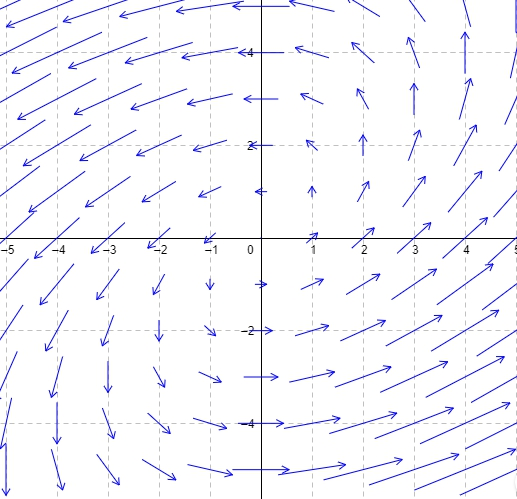
\includegraphics[width=60mm]{Images/ws21-c}\]

\item Vector fields $F$ in $\mathbf{R}^3$ of the form \[ F(x,y,z)=\dfrac{-k}{(x^2+y^2+z^2)^{3/2}} (x,y,z)\] ($k$ here is some constant) are commonly seen in physics as models of gravitational and electric fields. Describe the plot of this kind of vector field. 

Separately, describe the plot of the vector field $F(x,y)=(x^2-y^2-4, 2xy)$ in $\mathbf{R}^2$?
\end{enumerate}
Suggested additional exercises: \textit{Stewart} section 16.1

\section{Line integrals}

%\textit{Forewarning}: This is a long section with many different types of integral set-ups. One of the biggest challenges to understanding the upcoming material is understanding and using the notation correctly. Also, though we'll write what is about to follow for general $n$-dimensional space, we'll really only care about these for the cases $n=2$, $n=3$. You are free to mentally or physically replace $n$ by $2$ or $3$. 



In this section and throughout the remainder of the term we'll use the word \textbf{curve} to mean the trajectory of some smooth (see \ref{sec-smooth}) parametrized curve $r(t)$ in $\mathbf{R}^n$. Specifically, the domain of this curve is required to be a closed and finite interval $[a,b]$ of the real line (to avoid issues of improper integrals).  

Curves exist in the abstract: the main thing to know is that when we want to talk about an integral over a specific curve $C$, we need to first define a parametrization of $C$. 


\subsection{Line integrals of scalar functions} 

\begin{defn}[Line integral of a scalar function] Let $f$ be a continuous function $\mathbf{R}^n\to\mathbf{R}$ and $C$ be a curve in $\mathbf{R}^n$. We write  \begin{equation}  \int_C f \,ds\end{equation} for the \textbf{line integral of $f$ over $C$ with respect to arclength}. 
\end{defn} 
Note that $f$ does not have be defined on all of $\mathbf{R}^n$, just a suitably ``nice''\footnote{An open subset of $\R^n$ which contains $C$ is sufficient} region which contains the curve $C$. The differential $ds$ is called the \textbf{arclength differential} and conveys the information that we are to add this function $f$ up along the curve $C$ with respect to the \textit{length} of the curve. To compute it, we need to start with a parametrization $r(t)$ of the curve $C$, then \begin{equation} ds=|r'(t)|\,dt \end{equation}

\begin{defn} If $f$ is a continuous function $f\colon \mathbf{R}^n\to \mathbf{R}$, $C$ a curve in $\mathbf{R}^n$, and  $r(t)$ (for $t$ in $[a,b]$) is a parametrization of $C$, then: 

\begin{equation} \label{set-up-arclength-line-int}\int_C f \,ds = \int_a^b f\left( r(t) \right) |r'(t)|\,dt\end{equation}
\end{defn} 
Think of the right-hand side of \eqref{set-up-arclength-line-int} as the thing which evaluates the line integral $\int_C f\,ds$\footnote{Sometimes you'll see this called the \textit{pull-back} of the line integral (to $\mathbf{R}$).}. The thing to note here is that the right hand side of \eqref{set-up-arclength-line-int} is \textit{just} a normal (Riemann) integral of a one variable function: that is, these are the sorts of things we know how to evaluate using, say, the Fundamental theorem of calculus. 

In the particular case that $n=2$, \eqref{set-up-arclength-line-int} becomes
\begin{equation} \int_C f \,ds = \int_a^b f\left( x(t),y(t) \right) \sqrt{ x'(t)^2 +y'(t)^2 } \,dt\end{equation}
It's useful to know how to set up and interpret these different forms for line integrals. A good interpretation of these types of line integrals is that $f$ is a \textit{density} function and $\int_C f\,ds$ calculates mass of some thin wire. These types of integrals are sometimes called integrals of \textit{$0$-forms}

\begin{remark}It's worth bringing up that in \eqref{set-up-arclength-line-int} the \textit{choice} of parametrization of $C$ does not matter. This should be intuitively clear: the line integral depends on the curve, not the \textit{parametrization} of the curve; but is not immediately obvious on a more rigorous level. Nonetheless, we take this as given. You can think of sort of analogously to how we use Fubini's theorem for triple integrals: the choice of order $dx\,dy\,dz$ vs. $dy\,dz\,dx$ does not matter, it's just a convenience for how we choose to evaluate the thing that is the triple integral itself. \end{remark}




\subsection{Line integrals of vector fields} The second type of line integral we'll see is that of a \textit{vector field} over a curve $C$. Note that this is fundamentally a different type of object than a scalar function, so we'll need to figure out an appropriate description of a ``line integral'' of such a thing. 

\begin{defn}[Line integral of a vector field] Let $C$ be an oriented curve in $\mathbf{R}^n$ and $F$ be a vector field on $\mathbf{R}^n$. The \textbf{line integral of $F$ over $C$} is written
 \begin{equation} \int_C F\cdot d\vec{r}\end{equation}
 and represents the amount of \textbf{circulation} of the vector field $F$ along the curve $C$ in the given orientation.
 \end{defn} 
This requires unpacking: Let's say that $C$ is a curve in $\mathbf{R}^2$ and $r(t)=(x(t),y(t))$ a smooth parametrization of $C$ with domain $[a,b]$. We write $d\vec{r}$ for the \textbf{vector differential}\footnote{Really what's happening is we're seeing a new type of object. Differential geometers call these \textit{forms}, physicists may use the term \textit{tensor} (forms are an example of tensors, but not all tensors are forms). We'll refrain from requiring the use of the language of differential forms, but what we're calling vector fields are really just ``differential 1-forms"---that is, a smoothly varying collection of vectors just waiting to be integrated over a curve. The 1 in 1-form is essentially telling you these things can and should only be integrated over $1$-dimensional ``things" (manifolds) living inside the bigger space $\mathbf{R}^n$.} \[d\vec{r}:=(x'(t),y'(t)) \,dt=r'(t)\,dt\] (recall that $r'(t)$ is just the tangent vector to $C$).  The term $F\cdot d\vec{r}$ then represents the amount that $F$ ``goes in the direction" of $C$ when evaluated at a point on the curve. To integrate, we use the  parametrization $r(t)=(x(t),y(t))$ as follows: \begin{equation} \label{vector-line-int-2-alt}
	\int_C F\cdot d\vec{r}= \int_a^b F(x(t),y(t))\cdot (x'(t),y'(t))\,dt
\end{equation}
The right hand expression then tells us a bit more about what \textbf{circulation} means here: we're simply ``adding up" the amount which $F$ and the tangent vector $(x'(t),y'(t))$ to the curve go in the same direction over the curve. From here it's not too much trouble to write down a set-up for a line integral in $\mathbf{R}^n$. 

\begin{defn}[Line integrals of vector fields in $\mathbf{R}^n$] Let $F$ a vector field on $\mathbf{R}^n$ and $C$ a smooth curve in $\mathbf{R}^n$ given by the parametrization $r(t)$ for $a\leq t\leq b$. Then:
\begin{equation} \label{vector-line-int-3-alt}
	\int_C F\cdot d\vec{r}= \int_a^b F(r(t))\cdot r'(t)\,dt
\end{equation}
\end{defn}

\subsection{Other notation for line integrals of vector fields}
Recall that a vector field $F$ on $\mathbf{R}^n$ is made up of constituent functions: for instance, $F\colon \mathbf{R}^3\to \mathbf{R}^3$ is comprised of functions $f,g,h\colon \mathbf{R}^3\to\mathbf{R}$ such that \[ F(x,y,z)=\left(f(x,y,z), \, g(x,y,z), \,h(x,y,z)\right)\] (usually we suppress the input variables here for visual simplicity). Let $F=(f,g)$ be a vector field on $\mathbf{R}^2$ and $C$ a smooth curve in $\mathbf{R}^2$. Equivalent notation for the line integral $\displaystyle \int_C F\cdot d\vec{r}$ is to write the following: 
 \[\int_C F\cdot d\vec{r}= \int_C f \,dx+g\,dy \]


Here, $dx$ and $dy$ are really just the usual differentials we know and love from integral calculus. That is: if we have a parametrization $r(t)=(x(t),y(t))$ of $C$, then $dx=x'(t)\,dt$ and $dy=y'(t)\,dt$. We then have the following:
\begin{equation} \label{vector-line-int-2} \int_C F\cdot d\vec{r} =\int_C f\,dx + g\,dy= \int_a^b \left\lbrack f (r(t)) x'(t) + g(r(t)) y'(t) \right\rbrack\,dt\end{equation}


Similarly, if $F=(f,g,h)$ and $C$ is in $\mathbf{R}^3$ we have 
\[ \int_C F\cdot d\vec{r}= \int_C f \,dx+g\,dy+h\,dz\]
Given a choice of parametrization $r(t)=(x(t),y(t),z(t))$ of $C$ with domain $[a,b]$ we then have \begin{equation} \label{vector-line-int-3}
 \int_C f \,dx+g\,dy+h\,dz= \int_a^b \left\lbrack f(r(t)) x'(t)+ g(r(t)) y'(t)+h(r(t)) z'(t) \right\rbrack\,dt
\end{equation}

\begin{remark}Note that in all set ups \eqref{vector-line-int-2-alt}, \eqref{vector-line-int-3-alt}, \eqref{vector-line-int-2} and \eqref{vector-line-int-3} the terms on the right hand side are just ordinary integrals of (potentially complicated) 1 variable functions of $t$. These are functions we can integrate with the goold-old fundamental theorem of calculus. Consider these the ``set ups" of the given line integral. \end{remark}

\begin{remark}A good interpretation of these kinds of integrals is that $F$ is a force field (i.e., electromagnetic force, or force due to gravity) and $\int_C F\cdot d\vec{r}$ computes \textbf{work} of moving an object along path $C$. Terminology-wise, expressions of the form $f\,dx+g\,dy$, etc. are sometimes called integrals of \textit{$1$-forms} (here $1$ refers to the fact that these \textit{must} be integrated over $1$-dimensional ``things'' like curves, regardless of the dimension of the ambient space).\end{remark}

\subsection{Exercises}
\begin{enumerate}[label=\arabic*.]
\item Set up and evaluate the following line integrals with the given curve.

\begin{enumerate}
	\item $\displaystyle \int_C x^2y\,ds$ where $C$ is the unit circle $x^2+y^2=1$ starting at $(1,0)$ traveled once counterclockwise
	\item $\displaystyle \int_C xe^{yz} \,ds$ where $C$ is the line segment from $(0,0,0)$ to $(1,2,3)$
	\item $\displaystyle \int_C x/y \,ds$  where $C$ is the curve $x=t^3, y=t^4$ for $1\leq t\leq 2$.
	\item $\displaystyle \int_C x^2 \,dx + y^2\,dy$ where $C$ is the line segment from $(0,0)$ to $(3,4)$
	\item $\displaystyle \int_C z \,dx+ xy\,dy + y^2 \,dz$ where $C$ given by $r(t)=(\sin t, \cos t, \tan t)$ for $t$ in the interval $[-\pi/4 ,\pi/4]$
	\item $\displaystyle \int_C xy^2 \,dx  -x^2 \,dy$ where $C$ is given by $r(t)=(t^3,t^2)$ for $0\leq t\leq 1$
	\item $\displaystyle \int_C F\cdot d\vec{r}$ where $C$ is the unit circle $x^2+y^2=1$ starting at $(0,1)$ traveled once counterclockwise and $F(x,y)=(-y,x)$.
\end{enumerate}

\item A quarter circle of wire from the portion of the circle $x^2+y^2=9$ in the first quadrant. The wire is to have density given by $\rho(x,y)=xy$. Find the mass of the wire. (i.e., evaluate $\int_C xy\,ds$ where $C$ is the given quarter circle.)

\item \textit{Work} of moving an object through a force field $F$ along path $C$ is given by $\int_C F \cdot d\vec{r}$. Determine the work in moving an object along the parabola $y=x^2+1$ from $(0,1)$ to $(1,2)$ through force field $F(x,y)=(x^2,ye^x)$.

\item Given a curve $C$ in the plane let $-C$ denote the curve with the same trajectory but traversed in the opposite direction. Show that \[\int_C f\,ds= \int_{-C} f\,ds.\] Is it true that  $ \displaystyle \int_{-C} F\cdot  d\vec{r}=\int_C F\cdot d\vec{r}$?
\end{enumerate}


Suggested additional exercises: \textit{Stewart} Section 16.2 

\section{Conservative vector fields}

Our first observation is that by taking the gradient of any scalar function $f$, you produce a vector field. For instance if $f(x,y,z)=xy^2+2z$ then $\nabla f(x,y,z)= (y^2, 2xy, 2)$. We'll see that vector fields which originate this way are ``special''.

\begin{defn}[Conservative vector field] Let $F$ be a vector field on $\mathbf{R}^n$. $F$ is called \textbf{conservative} if there is a scalar function of $n$ variables $\varphi$ such that \begin{equation} F=\nabla \varphi \end{equation}

%Any vector field which can be identified as the gradient of some scalar function is called a \textit{conservative vector field}. If a vector field $F$ is given by the gradient of some scalar function $\varphi$, we call $\varphi$ a \textit{potential function} of $F$. 
 % Line integrals of the form $\int_C F \cdot d\vec{r}$ where $F$ is a conservative vector field have some special properties. 
\end{defn}
Terminology-wise, if $F=\nabla \varphi$ we call $\varphi$ a \textbf{potential function}\footnote{This terminology is motivated by physics---potential is as in \textit{potential energy}.} for $F$. A more mathematically motivated word is to call such vector fields \textbf{exact}.

\subsection{Computing potential functions} Suppose that $F=(f,g)$ is a vector field on $\mathbf{R}^2$. Note that if $F$ is conservative, then $f=\varphi_x$ and $g=\varphi_y$ for some scalar function $\varphi$. Therefore, solving for \textit{a} potential function of $F$ amounts to solving the system of differential equations: \begin{equation} f=\varphi_x, \;g=\varphi_y\end{equation} Though this may sound intimidating, no real advanced techniques from differential equations are required. One method is to do the following: Whatever $\varphi$ is, it must be an antiderivative of $f=\varphi_x$ with respect to $x$. So you can write \[ \varphi(x,y)= \int f \,dx+c(y)\] where $c(y)$ is some function which just depends on $y$. Then, you can solve for $c(y)$ by taking $y$ partials on both sides, equating \[ g=\varphi_y=\dfrac{\partial}{\partial y} \left( \int f\,dx + c(y)\right)\]
With functions of more variables, the same idea is employed, a ``zig-zag'' of integrating and differentiating with respect to the different variables. 

\subsection{Line integrals of conservative vector fields}

\begin{thm}[Fundamental theorem of line integrals] \label{ftc-line-int} Suppose that $F$ is a conservative vector field in $\mathbf{R}^n$ and that $\varphi$ is a potential function for $F$. Let $C$ be a (smooth) curve from point $A$ to $B$ in $\mathbf{R}^n$. Then: \begin{equation} \label{ftc} \int_C F \cdot d\vec{r}= \varphi(B)-\varphi(A)\end{equation}
\end{thm}
Note how this bears a resemblance to the familiar Fundamental theorem of calculus for $1$-variable functions\footnote{That is, if $f$ is a continuous function on $[a,b]$ and $g$ is a function such that $g'(x)=f(x)$ (i.e., an antiderivative) for all $x$, then \[\int_a^b f\,dx=g(b)-g(a)\]}. This turns the problem of evaluating certain types of line integrals into a problem of solving a system of differential equations to find a potential function of $F$. 


\begin{remark} There are some fairly useful and interesting implications of theorem \ref{ftc-line-int}. Let $F$ be a conservative vector field on $\mathbf{R}^n$ with potential function $\varphi$, and $C$ a (smooth) curve between points $A,B$. Then: 
\begin{enumerate}[label=\roman*.]
	\item The \textit{path} that $C$ takes from points $A$ to $B$ does not actually matter---just the value of the potential function of the vector field at the end points. Whenever a line integral of a given vector field $F$ has this property we say that the value of $\int_C F\cdot d\vec{r}$ is  \textbf{path independent}. Line integrals of conservative vector fields over smooth curves are always path independent. 
	
	\item \label{closed-path-int} Let's say that a a curve $C$ is \textbf{closed} if the start and end points of $C$ are the same. Then if $F$ is conservative and $C$ a closed path, we must have \begin{equation} \int_C F \cdot d\vec{r}=0\end{equation} This follows readily from theorem \ref{ftc-line-int}: if the end points of $C$ are the same, then $\varphi(B)=\varphi(A)$, so $\varphi(B)-\varphi(A)=0$. 
	
	\item If $F$ is \textit{any} vector field, then the statement that $\int_C F\cdot d\vec{r}$ is path independent is equivalent to the property that $\int_C F\cdot d\vec{r}=0$ for any closed curve $C$. (This is worth checking for yourself)
	
	\item The converse to \ref{closed-path-int} is also true: If $\int_C F\cdot d\vec{r}=0$ for \textit{all} closed paths $C$ in some region $R$ then $F$ is conservative (on the domain $R$)\footnote{This is a bit trickier to show, but the idea is as follows: Since $\int_C F\cdot d\vec{r}=0$ for all closed curves $C$, then $\int_C F\cdot d\vec{r}$ must be path independent. Fix a basepoint $P$ in $R$ and let $B$ be any point in $R$. Define $\varphi(B)=\int_C F\cdot d\vec{r}$ for $C$ some path from $P$ to $B$. Since $\int_C F\cdot d\vec{r}$ is path independent, this produces a well-defined function $\varphi$. The claim is then that $\varphi$ must be a potential function for $F$.}.
	

%	\item If a vector field $F=(f,g)$ is continuous in some domain $D$ of $\mathbf{R}^2$ then $f_y=g_x$ for all points in $D$. The converse is true if the domain $D$ is \textit{simply connected} (i.e., has no holes\footnote{This observation is sort of the beginning of the field of algebraic topology...or at least one of them}). 
\end{enumerate}
\end{remark}

It's worth pointing out that sometimes you'll see the notation \[\oint_C F\cdot d\vec{r}\] used for line integrals over a \textit{closed} path $C$, use this if you like, but use it correctly (i.e., don't write this unless you know the path is really closed).



\begin{thm}[Equivalent conditions for conservativeness of a vector field] Let $F$ be a vector field defined on a region $R$ in $\mathbf{R}^n$. The following statements are equivalent.
\begin{enumerate}[label=(\arabic*)]
	\item $F$ is a conservative vector field
	\item $\displaystyle \int_C F\cdot d\vec{r}$ is path independent for all smooth curves $C$ in the domain of $F$
	\item $\displaystyle \oint_C F\cdot d\vec{r}=0$ for all closed paths $C$ in $R$. 	
\end{enumerate}
\end{thm}
There's one more statement to add to this list but it's specific to $\mathbf{R}^2$ and will take a bit of set-up. 

\subsection{Test for conservativeness of a vector field on $\mathbf{R}^2$} Knowing whether a given vector field is conservative or not is fairly useful, as it then tells us meaningful things about line integrals of that vector field. How then to determine if a vector field is actually conservative? Solving for a potential function is certainly one way, but can rely on solving difficult integrals to produce a function explicitly.

Suppose that a vector field $F=(f,g)$ is given. If $F=\nabla \varphi$ then we would need to have $f=\varphi_x$ and $g=\varphi_y$ as in . In particular then, by Clairut's theorem (theorem \ref{Clairut-thm}), the component functions $f$ and $g$ need to satisfy \begin{equation} \label{curl-free} f_y=g_x \qquad \qquad\end{equation} since both are equal to $\varphi_{yx}=\varphi_{xy}$. 
This brings us to the next definition.

\begin{defn}[2D curl]Let $F=(f,g)$ be a vector field on $\mathbf{R}^2$ such that $f,g$ are differentiable functions. Define the \textbf{2D-curl} of $F$ by \begin{equation} \curl_{2D} F=g_x-f_y\end{equation}\end{defn}

This gives us a two-variable function $\curl_{2D} F$ which represents the \textbf{instantaneous rotation} of the vector field $F$ at a point in its domain. Said more explicitly, given a point $P$ 
\begin{itemize}
	\item If $\curl_{2D}F(P)>0$ then $F$ is has \textit{instantaneous counterclockwise rotation} at $P$
	\item If $\curl_{2D}F(P)<0$ then $F$ is has \textit{instantaneous clockwise rotation} at $P$
	\item If $\curl_{2D}F(P)=0$ then $F$ has \textit{no instantaneous rotation} at $P$
\end{itemize}
The last case is useful to have a word for, so let's also define the following
\begin{defn} \label{def-curl-free} Let $F=(f,g)$ such that $f,g$ are differentiable functions in some region $R$ in $\mathbf{R}^2$. We say that $F$ is \textbf{curl-free}\footnote{Sometimes also called \textit{closed}, however this word is hilariously overused} if $f_y=g_x$. 
\end{defn}

Equivalently, a vector field $F$ is curl-free if $\curl_{2D}F=0$. Any conservative vector field on $\mathbf{R}^2$ is necessarily curl-free. The converse is true on particular types of regions, and a precise definition of what types of regions work here requires a bit of terminology from \textit{topology}. 

\begin{defn}Let $R$ be a region in $\mathbf{R}^2$. We say that $R$ is simply connected if $R$ has no \textit{holes} in it. \end{defn}

\begin{remark} \textit{Makes sense}? Maybe not quite. A more precise definition of what this should mean is beyond the scope of what we'll need in this class\footnote{The right tool here is the \href{https://en.wikipedia.org/wiki/Fundamental_group}{\textit{fundamental group}} of a topological space.}, but we'll be able to at least diagnose simply-connectedness visually. For instance, of the two regions in Figure \ref{fig-simpl}, the one on the left is simply connected, while the one on the right is not\footnote{The old joke is that this shape is just a t-shirt---can you tell why?} 

\begin{figure}[h!]
\centering 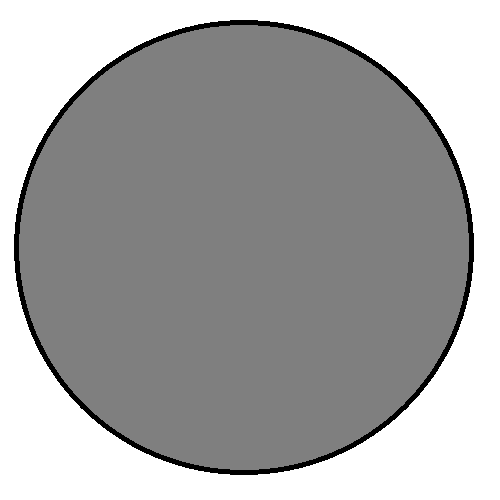
\includegraphics[width=45mm]{Images/sc} \qquad \qquad 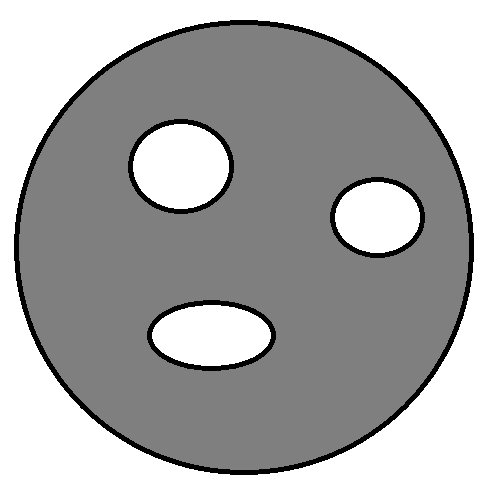
\includegraphics[width=45mm]{Images/nsc}
\caption{Simply connected region (left), non-simply connected region (right)}
\label{fig-simpl}
\end{figure}

For instance, $\mathbf{R}^2$ is simply connected, as are each of the quadrants in $\mathbf{R}^2$. The ur example of a non-simply connected region is $\mathbf{R}^2$ with a point removed. 
 \end{remark}

%So, we can then finally add the last equivalent statement to the theorem above (given that $F$ is a vector field in $\mathbf{R}^2$, at least). 


\begin{thm}[Equivalent condition for conservativeness of a vector field in $\mathbf{R}^2$]
Let $F$ be a vector field defined on a region $R$ in $\mathbf{R}^2$. If $F$ is curl free and $R$ is simply connected, then $F$ is conservative.
\end{thm}


\subsection{Exercises}
\begin{enumerate}[label=\arabic*.]

\item For each of the following, determine if the given vector field is conservative. If it is, find a potential function for it. 

\begin{enumerate}
	\item $F(x,y)=( xy+y^2, x^2+2xy)$
	\item $F(x,y)=(ye^x, e^x+e^y)$
	\item $F(x,y)=(-y,x)$
	\item $F(x,y)=(\ln y +y/x, \ln x+x/y)$
\end{enumerate}

\item Use the fundamental theorem of line integrals to evaluate the following line integrals

\begin{enumerate}
	\item $\displaystyle \int_C 2x \,dx + 4y \,dy$ where $C$ is the arc of the parabola $y=x^2$ from $(0,0)$ to $(2,4)$.
	\item $\displaystyle \int_C (3+2xy^2)\,dx+ 2x^2y\,dy$ where $C$ is the line segment between $(1,1)$ and $(3,14)$
	\item $\displaystyle \int_C \sin y \,dx + (x\cos y+\cos z) \,dy-y \sin z\,dz$ where $C$ is the segment of the helix $r(t)=(\cos t, \sin t, 3t)$ for $0\leq t\leq 5$.
\end{enumerate}

\item Vector fields of the form \[ F(x,y,z)= \dfrac{k}{(x^2+y^2+z^2)^{3/2}} (x,y,z)\] are of important use in physics (examples include electromagnetic and gravitational force fields), where $k$ is some constant. Show that \[\varphi(x,y,z)= \dfrac{-k}{(x^2+y^2+z^2)^{1/2}}\] is a potential function for $F$. Use this to find the work done in moving an object from point $(1,0,-1)$ to $(0,2,0)$ through the vector field $F$ (leave you answer in terms of $k$). 

\item For each of the following, sketch the region of the $xy$-plane determined by the set and determine if the given set is simply-connected. 

\begin{enumerate}
	\item $\{ (x,y) \, | \, (x,y)\neq (2,3) \}$ 
	\item $\{ (x,y) \, | \, 1 < |x| < 5, x^2+y^2\geq 4 \}$
	\item $\{ (x,y) \, | \, 0< y< 3, 0< x< 10\}$	
\end{enumerate}

\item Show that if $f,g,h$ are functions with continuous first-order derivatives and $F=(f,g,h)$ a vector on $\mathbf{R}^3$ is conservative i.e., there is a scalar function $\varphi$ with $F(x,y,z)=\nabla \varphi(x,y,z)$ for all $(x,y,z)$ that \[ f_y=g_x, f_z=h_x, \text{ and } g_z=h_y.\] (\textit{Question: Why do we need the first condition about continuous first order derivatives?})

\item \textit{True or false}. Determine if the following statements are true or false. Give a brief justification of your answer

\begin{enumerate}
	\item The following vector field is conservative 
	
		\[ 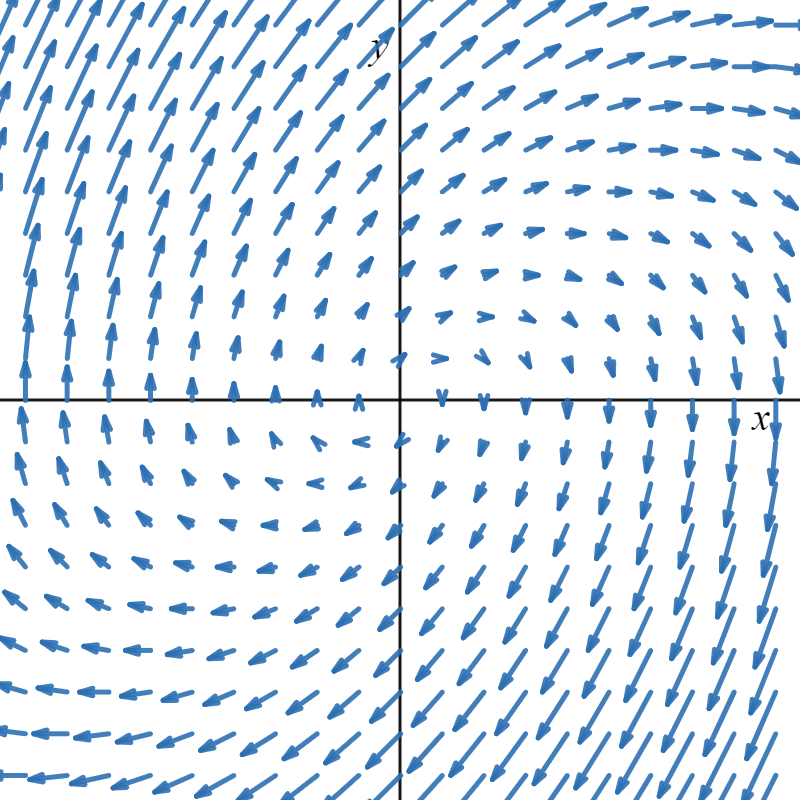
\includegraphics[width=60mm]{Images/ws9-vf}\]

	\item If $F=(f,g)$ is a vector field defined and continuous on all of $\R^2$ with $f_y=g_x$ then $F$ must equal $\nabla \varphi$ for some potential function $\varphi$
	
	\item If there is a closed curve $C$ with $\int_C F\cdot d\vec{r}=0$ then $F$ must be conservative
	
	\item If $a,b$ are constants such that the vector field $F(x,y)=(ay,bx)$ is conservative then $a=b$. 
\end{enumerate}

\end{enumerate}
Suggested additional exercises: Section 16.3 

\section{Green's theorem}

Green's\footnote{It's worth reading up on \href{https://en.wikipedia.org/wiki/George_Green_(mathematician)}{George Green}. He was self-trained in mathematics and wholly unappreciated in his time, it's a remarkable story how Green's theorem name came to be named after him.}  theorem is the first instance of the ``stuff on inside of region'' equals ``stuff on boundary'' phenomenon we see with a region that is two dimensional (while this may not make perfect sense now, hopefully it does by the end of the term). The slogan for Green's theorem is that \textit{total circulation} (the left hand side of \ref{green}) of a vector field over a closed curve $C$ is equal to the sum (double integral on the right of \ref{green}) of \textit{circulation density} (i.e., 2D curl) over the 2D region bounded by $C$. 
\begin{figure}[h!]
\centering
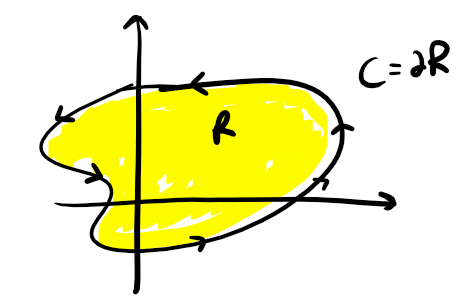
\includegraphics[width=70mm]{Images/greens-region}
\caption{A closed simple curve $C$ bounding a region $R$ (yellow)}
\label{fig-greens-curve}
\end{figure}
%:
\begin{thm}[Green's theorem]\label{thm-green}If $C$ is a positively oriented, piecewise smooth, closed, simple curve in $\mathbf{R}^2$, $R$ the region enclosed by $C$, and $f,g$ functions with continuous first order derivatives on $R$, then: \begin{equation} \label{green} \int_C f\,dx+g\,dy=\iint_R (g_x-f_y)\,dA.\end{equation}

\end{thm}




There's a lot of adjectives here describing the curve $C$, which are defined below. Let's call a curve which meets al of these conditions ``good''.
\begin{itemize}

	\item \textbf{piecewise smooth} means $C$ has a parametrization which is smooth except at perhaps finitely many points (think of these like places where a piecewise function changes definition). Unless otherwise mentioned, we always assume our curves are piecewise smooth. 
	\item \textbf{closed} means $C$ starts and ends at the same point.
	\item \textbf{simple} means $C$ has no self-intersections (except for \textit{possibly} the start and end point).
	\item \textbf{positively oriented} means $C$ is oriented \textit{counter-clockwise} (meaning if you can deform $C$ to a circle without breaking or tearing the path, then the corresponding circle is parametrized counter-clockwise). Note that this term really only makes sense when talking about a closed, simple curve. 
\end{itemize}

\begin{figure}[h!]
\centering
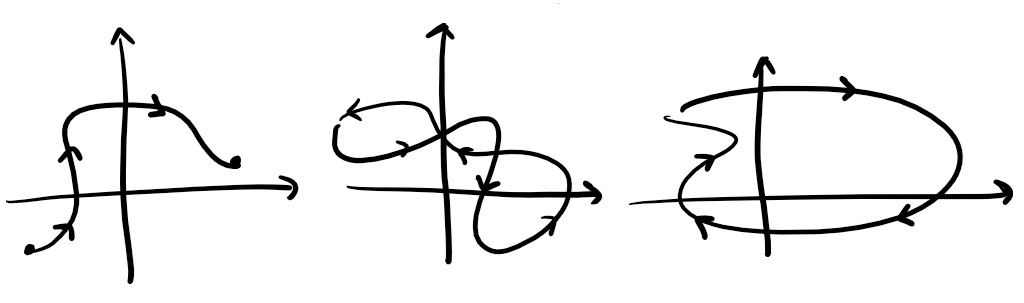
\includegraphics[width=150mm]{Images/curves-not-green}
\caption{Left to right: A curve which is not closed; a curve which is not simple; a curve which not positively oriented.}
\label{fig-curves-ex}
\end{figure}


\begin{remark}It's actually a somewhat deep theorem that \textit{any} closed simple curve will split the plane into an inside and outside\footnote{This is called the \href{https://en.wikipedia.org/wiki/Jordan_curve_theorem}{Jordan curve theorem}.} but at least drawing a few examples we can empirically verify it. If $C$ is such a curve, and $R$ the corresponding enclosed region, we also write\begin{equation} C=\partial R \end{equation} and call $C$ the \textbf{boundary} of $R$. 
Another, equivalent, way of writing Green's theorem is that \[ \int_{\partial R} F\cdot d\vec{r}=\iint_R \curl_{2D} F\,dA\] 
\end{remark}
\begin{example}[Relation to curl-free vector fields]Green's theorem also gives us another way of interpreting the relation between \textit{curl-free} (see def. \ref{def-curl-free}) vector fields and their line integrals over closed paths. Note that if $F=(f,g)$ is curl free (i.e., $f_y=g_x$), then the integrand $g_x-f_y$ for the double integral in \eqref{green} is just identically $0$ inside $R$. So, if $C$ is a closed path bounding $R$ then, \begin{equation} \int_C F\cdot d\vec{r}=\int_C f\,dx+g\,dy=\iint_R (g_x-f_y)\,dA=\iint_R 0 \,dA=0\end{equation}
\end{example}

\subsection{Relation to the Fundamental theorem of calculus}One thing to note is that for an interval $[a,b]$ we have \[\partial [b,a]=\{ b^+, a^-\}\] where $b^+$ means the point $b$ signed \textit{positively} and $a^-$ means $a$ signed \textit{negatively}. In particular, the expression $(g_x-f_y)\, dA$ behaves somewhat like the ``derivative'' of the vector field $f\,dx+g\,dy$, so \eqref{green} can be interpreted as an expression of the form \[ \int_{\partial D} \text{stuff} = \iint_D \text{derivative of stuff}.\] 
In particular, this should reminiscent of the Fundamental theorem of calculus (from Calc 1) (and also the Fundamental theorem of line integrals, theorem \ref{ftc-line-int}). Since integrals are, at their core, just (continuous) sums, we have the following heuristic understanding of FTC in this context:
\[ \int_{\partial [a,b]} g\,dx =g(b)-g(a)=\int_a^b g'(x)\,dx= \int_{[a,b]}g'\,dx \]
(\textit{can you make the correlation also with the fundamental theorem of line integrals we saw in the last section?}) This is the general theme we'll see with the remaining theorems in this term. In particular, later we'll see that Green's theorem \eqref{green} is really just a special case of a more general theorem (Stokes' theorem\footnote{Which is also a specific case of something else called Stokes' theorem.}).


\subsection{Flux form of Green's theorem} \label{flux-form-greens}
Let $F$ be a vector field and $C$ a closed curve in $\mathbf{R}^2$. We know that $ \int_C F \cdot d\vec{r}$ represents the total circulation of $F$ on $C$, i.e., how much $F$ \textit{rotates} over the region. A complementary piece of information we can measure is the \textbf{flux} (i.e., flow) of this vector field \textit{through} the curve $C$. 

Given a closed simple curve $C$, let's let $\vec{n}$ be the \textit{outward} normal vector\footnote{Note this is different from the \textit{principal normal vector} $N$ we saw with \eqref{unit-normal}. You can relate the two, but it doesn't really matter for what we're trying to accomplish.}. That is, $\vec{n}$ points away from the region which $C$ bounds. 
\begin{defn}[Flux of a vector field over a curve in $\mathbf{R}^2$]
	Let $F$ be a vector field and $C$ a closed simple curve in $\mathbf{R}^2$. Let $\vec{n}$ be the outward normal vector for $C$. The (outward) \textbf{flux} of $F$ over $C$ is the expression \begin{equation} \int_C F\cdot d\vec{n} \end{equation}
\end{defn}
Outward flux represents the amount which $F$ ``flows" out of the region bound by $C$. If $\int_C F\cdot d\vec{n}$ is positive, then the vector flows \textit{out} (think water overflowing a cup, the curve is the rim of the cup), if negative the vector field flows \textit{in}.

\begin{figure}[h!]
\centering
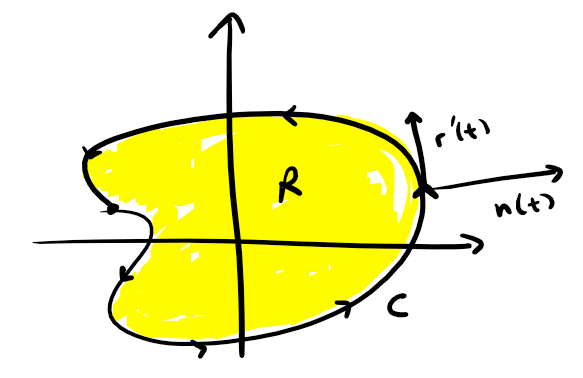
\includegraphics[width=70mm]{Images/normal-greens}
\caption{Outward normal vector $\vec{n}$ for a closed, simple, positively oriented curve} 
\label{fig-n-from-r}
\end{figure}


How to calculate? Here's a neat observation: If $\vec{r}(t)=(x(t),y(t))$ is a parametrization of $C$ in the positive orientation, then $\vec{n}$ is given by\footnote{If you know a bit about rotation matrices this is not so hard to show. Here, $\vec{n}$ is the result of applying the transformation \[T=\begin{pmatrix} 0 & 1 \\ -1 & 0\end{pmatrix}\] to $\vec{r}$. Here, $T$ is just the ``rotate by angle $\pi/2$ clockwise" transformation for vectors in $\mathbf{R}^2$. This is exactly the rotation needed to turn $\vec{r}\,'$ into $\vec{n}$.} (see Figure \ref{fig-n-from-r}) \begin{equation} \vec{n}(t)=(y'(t),-x'(t))\end{equation}


So, given a (positively oriented) parametrization $r(t)$ of $C$ with domain $[a,b]$, the (outward) flux of $F$ over $C$ is calculated by \begin{equation} \int_C F\cdot d\vec{n} = \int_a^b F(r(t))\cdot (y'(t),-x'(t))\,dt\end{equation}

That is to say, the outward flux is just a line integral over $C$. Which means, we can apply Green's theorem to this line integral. Let's suppose $F$ has component functions $F=(f,g)$
\begin{align*}
	\int_C F\cdot d\vec{n} & = \int_C F(r(t))\cdot (y'(t),-x'(t))\,dt \\
	& = \int_C \left( f(r(t)) y'(t) - g(r(t))x'(t) \right) \,dt\\
	& =\int_C  -g\,dx+f\,dy \\
	& = \iint_R (f_x-(-g_y))\,dA 
\end{align*}
where the last step comes from Green's theorem \eqref{green}. We can summarize this with the \textit{flux form} of Green's theorem

\begin{corr}[Flux form of Green's theorem]\label{green-flux}
Let $C$ a closed simple curve in $\mathbf{R}^2$ bounding a region $R$, $\vec{n}$ the outward normal vector for $C$, and  $F=(f,g)$ a vector field such that $f,g$ have first order derivatives which are defined and continuous on $R$. Then \begin{equation} \label{div-2} \int_{C} F\cdot d\vec{n} = \iint_R (f_x+g_y) \,dA\end{equation} 
\end{corr}
The expression $f_x+g_y$ that we see in the right hand side of \eqref{div-2} is called the \textbf{divergence} of $F$. We'll see more examples of divergence, and how to extend it to higher dimensions, in later sections. 


\subsection{Exercises}
\begin{enumerate}[label=\arabic*.]

\item Use Green's theorem to evaluate the following:

\begin{enumerate}
	\item $\displaystyle \int_C ye^x\,dx+2e^x\,dy$ where $C$ is the rectangle with vertices $(0,0), (3,0), (3,4)$ and $(0,4)$.

	\item $\displaystyle \int_C y^3\,dx+x^3\,dy$ where $C$ is the circle $x^2+y^2=4$.
	\item $\displaystyle \int_C x^2y^2\,dx + y\arctan(y)\,dy$ where $C$ is the triangle with vertices $(0,0), (1,0)$ and $(1,3)$. 
\end{enumerate}

\item Let $C$ be the curve (oriented positively) in the following picture. 

\[ 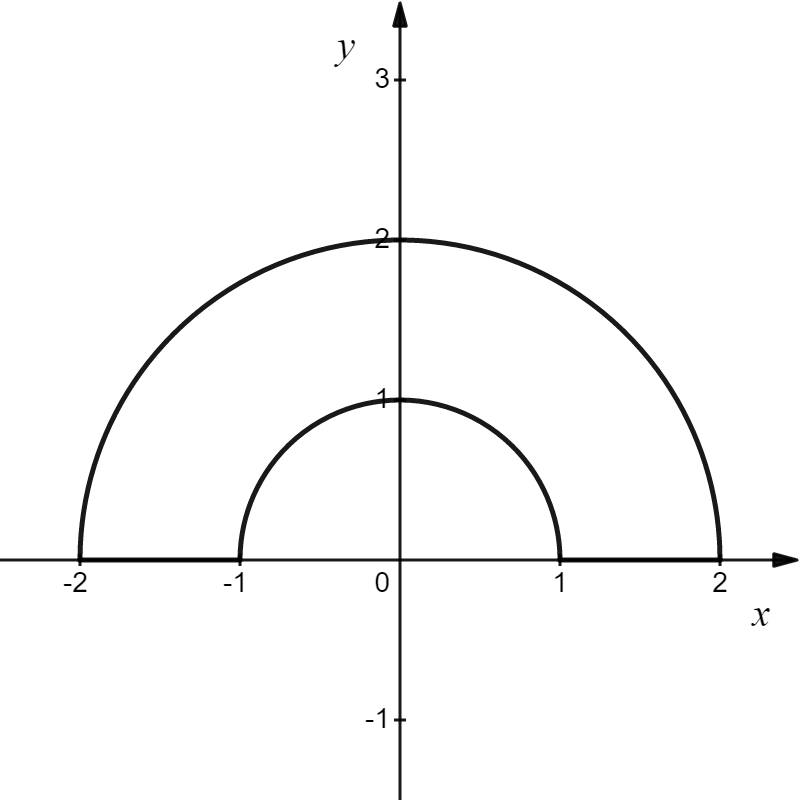
\includegraphics[height=60mm]{Images/ws10-arc}\]

Use Green's theorem to evaluate $\displaystyle \int_C y^2\,dx + 3xy\,dy$. (\textit{Hint: use polar coordinates for the double integral over the region.})


\item Use Green's theorem to show the following



\begin{enumerate}

\item If $F=(f,g)$ is a conservative vector field and $C$ a ``good'' curve, then \[\int_C F\cdot d\vec{r}=0\]
\item If $D$ is a region with $\partial D$ a ``good'' curve, then\footnote{There's actually a nifty device that makes use of this called a \href{https://en.wikipedia.org/wiki/Planimeter}{planimeter}.} \[ \text{area of $D$}= \int_{\partial D} x\,dy=-\int_{\partial D}y\,dx\]
 
\item If $D$ is a region with $\partial D$ a ``good'' curve, then \[ \bar{x}=\dfrac{1}{2(\text{area of $D$})} \int_{\partial D} x^2\,dy \qquad \bar{y}=-\dfrac{1}{2(\text{area of $D$})} \int_{\partial D} y^2\,dx\]
(\textit{here $\bar{x}$ and $\bar{y}$ denote the coordinates of the \textit{centroid} of $D$}.)
\item If $C$ is the line segment between points $(a,b)$ and $(c,d)$ in $\mathbf{R}^2$ then \[ \int_C x\,dy - y\,dx= ad-bc=\det\begin{pmatrix} a & b \\ c & d\end{pmatrix}\]
\end{enumerate}
\item Use 3b. to show that the area of the ellipse $\dfrac{x^2}{a^2}+\dfrac{y^2}{a^2}=1$ is $\pi ab$. 

\item \textit{True or false}. If $C$ is a ``good'' curve enclosing a region $D$, then $D$ must be simply connected. 
\end{enumerate}

Suggested additional exercises: \textit{Stewart} section 16.4



\section{Surface integrals}

We focus now (and for the remainder of the term pretty much) on surfaces in 3 dimensional space $\mathbf{R}^3$. The first step is understanding \textit{how} to parametrize a surface and what such functions look like. Recall that a \textit{parametric curve} is a function $r\colon \mathbf{R}\to \mathbf{R}^n$, that is, a function $r(t)$ defined by component functions $x(t), y(t)$ (and possibly $z(t)$, etc.). 

A \textit{parametric surface} is the same idea, but with input ``$t$'' replaced by two variables (generically we use the letters $u$ and $v$ but not necessarily always). What this gains us from, say, just an equation of the surface, is to allow us talk about ``stuff'' on the surface. For instance, this ``stuff'' could be a function that'd we'd like to integrate.

\begin{figure}[h!] 
\centering
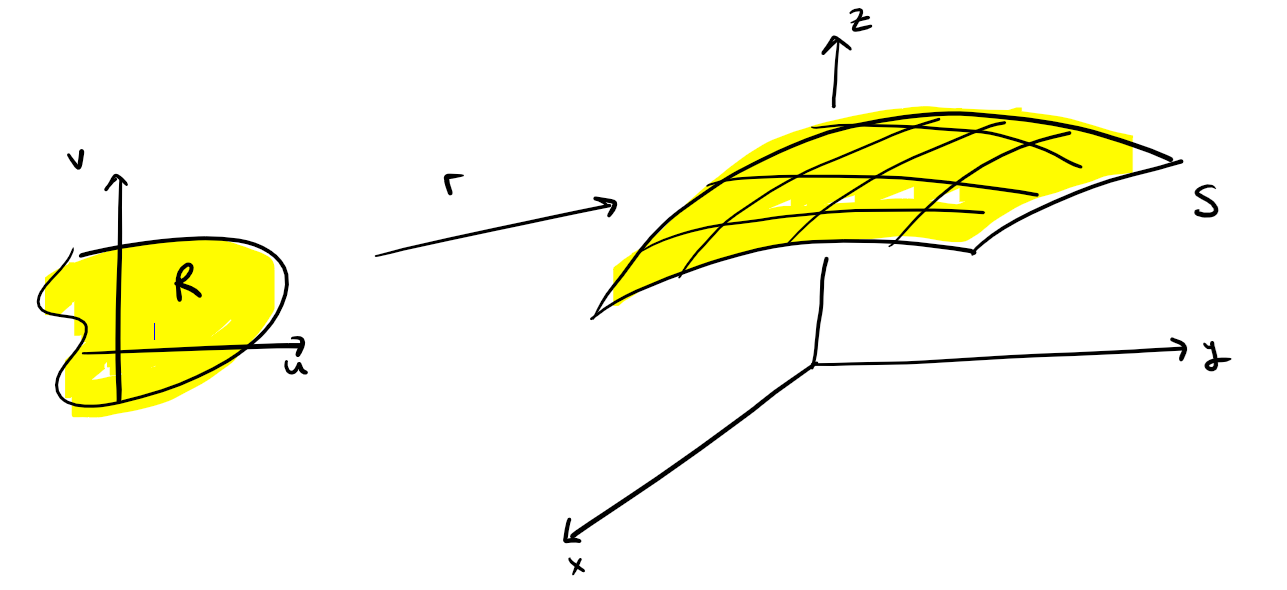
\includegraphics[width=150mm]{Images/surface-r}
\caption{Parametrization $r$ of surface $S$ with domain $R$.}
\label{fig-surface-param}
\end{figure}

\begin{defn}[Parametric surface] Let $S$ be some surface in $\mathbf{R}^3$ given by the implicit equation $F(x,y,z)=0$. A \textbf{parametrization} of $S$ is a function $\vec{r}\colon R\to \mathbf{R}^3$ defined by component functions \begin{equation} \vec{r}(u,v)=\left(x(u,v), y(u,v), z(u,v)\right)\end{equation}
for points $(u,v)$ within some domain $D$ in $\mathbf{R}^2$ such that \begin{itemize}
\item  $F(x(u,v),y(u,v),z(u,v))=0$ for all point $(u,v)$ in the domain of $r$
\item The range of $r$ is $S$. 
\end{itemize}
\end{defn}
That is to say, the component functions of the parametrization must satisfy the equation to be on $S$, and must cover all of $S$. For the types of surfaces we're considering we'll usually require that the component functions should have partial derivatives $x_u,x_v$, etc existing whenever necessary. 

When useful to distinguish it as a vector, we can decorate the parametrization with the vector-hat, $\vec{r}$, though this is not entirely necessary. The key is that the notation should be \textit{useful} to you, but not overly burdensome to write.

\begin{example}[Parametrization of a sphere] Consider the surface $S$ that is the unit sphere $x^2+y^2+z^2=1$ in $\mathbf{R}^3$. A parametrization of $S$ comes from our spherical coordinate substitution with $\rho=1$. That is, \begin{equation} \vec{r}(u,v)=(\sin u\cos v, \sin u\sin v, \cos u) \qquad 0\leq u\leq 2\pi, 0 \leq v \leq \pi\end{equation}
It's worth checking for yourself that for this parametrization that  \[(x(u,v))^2+(y(u,v))^2+(z(u,v))^2=1\] for all points $u,v$ and that the (outward) normal vector $\vec{n}$ (see \eqref{unit-normal}) is given by \begin{equation} \vec{n}(u,v)=(\sin^2 u\cos v, \sin^2 u\sin v, \sin u\cos u).\end{equation} What's more is that you can easily modify this to be a parametrization of any sphere: the sphere of radius $k$ with center at point $(a,b,c)$ is parametrized by \begin{equation} r(u,v)=(a+k\sin u \cos v, b+k\sin u \sin v, c+k\cos v)\end{equation} and has (outward) normal vector given by \begin{equation} r_u\times r_v= (k^2\sin^2 u\cos v, k^2\sin^2 u\sin v, k^2\sin u\cos u)
\end{equation}
\end{example}

\subsection{Non-degenerate surfaces} In the same way that we can only integrate over a smooth curve, we must have a similar condition for surfaces. This is called a \textbf{non-degenerate surface} (also called a \textbf{smooth} surface).  

\begin{defn}[Non-degenerate surface] Let $r(u,v)$ be a parametrization of a surface $S$. A parametrization $r=r(u,v)$ of a surface $S$ is called \textbf{non-degenerate} if these tangent vectors are not parallel, or equivalently if $r_u \times r_v$ is not the zero vector. 
\end{defn}
The idea is that, when evaluated at a point, the partial derivatives $r_u$ and $r_v$ produce two vectors which are both tangent to the surface $S$. If these vectors happen to be parallel there is a ``dimension collapse" or redundancy in the parametrization, making the surface $S$ not really 2-dimensional. Since $r_u,r_v$ are necessarily vectors in $\mathbf{R}^3$ we can use that vectors are parallel and only if their cross-product is not the zero vector to phrase non-degeneracy as $|r_u \times r_v|\neq 0$. Unless stated otherwise, we'll only be considering non-degenerate parametrizations. 

\begin{figure}[h!]
\centering
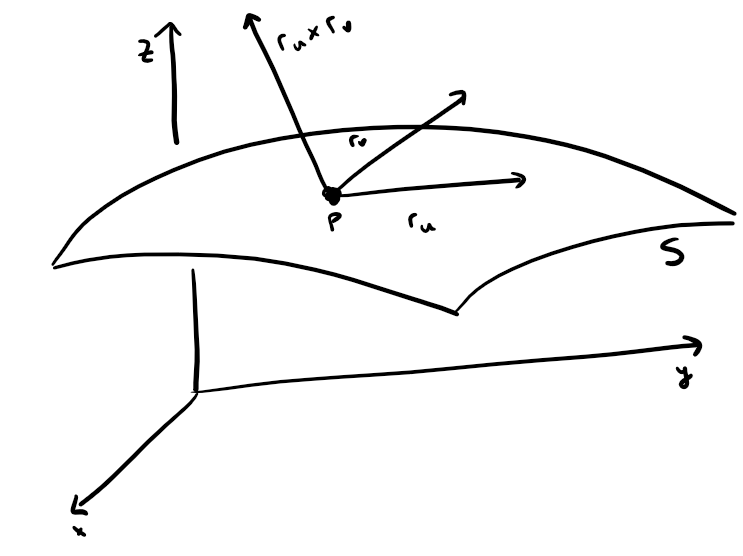
\includegraphics[width=90mm]{Images/surface-normal}
\caption{Tangent vectors $r_u,r_v$ and normal vector $r_u\times r_v$ to a parametrized surface $S$.}
\label{fig-surface-normale}
\end{figure}
\begin{remark}Let $S$ be a non-degenerate surface parametrized by $r=r(u,v)$ on domain $D$ in $\mathbf{R}^2$. Some useful observations:

\begin{itemize}
	\item Since the cross product of two vectors is always orthogonal to both, we can use the tangent  vectors $r_u,r_v$ to compute a \textbf{normal vector} to $S$ as follows (see also Figure \ref{fig-surface-normale}): \begin{equation} \label{unit-normal} \vec{n}=r_u \times r_v \end{equation}
	As a corollary, the \textit{tangent plane} to $S$ at point $r(u,v)$ is given by \[\vec{n}(u,v) \cdot ((x,y,z)-r(u,v))=0.\]

	\item Furthermore, the magnitude of the cross product gives us the appropriate ``skewing factor'' of area when viewing a small rectangle in $u,v$ on the surface itself. The \textbf{surface area} of $S$ is computed by \begin{equation} \label{SA}  \iint_D |r_u \times r_v| \,dA\end{equation}
	
	\item One of the nicest cases is when $S$ arises as the graph $z=f(x,y)$ of a two variable function $f$. In this case, $r(u,v)=(u,v,f(u,v))$ is a parametrization of $S$. 
	
	We can then check: \[ \vec{n} = (-f_u,-f_v,1) \] and surface area is given by  \begin{equation} \label{eq-SA} \iint_S 1\,d\sigma= \iint_D \sqrt{ 1+ (f_u)^2+(f_v)^2 }\,dA\end{equation}

	%\item If $r(u,v)=(x(u,v),y(u,v), z(u,v)$ defines a surface $\sigma$ and $f(x,y,z)$ a continuous function whose domain includes $\sigma$, then the \textit{surface integral} of $f$ is computed as: \[ \iint_{\sigma} f\,dS = \iint_D f \left( x(u,v), y(u,v), z(u,v) \right) |r_u \times r_v| \,dA \]
\end{itemize}
\end{remark}




\subsection{Surface integrals of scalar functions} Let's stick with the assumptions that $S$ is a surface in $\mathbf{R}^3$ given by a non-degenerate parametrization $r=r(u,v)$ on domain $D$.  As with line integrals, we'll experience two similar, but distinct in style, types of surface integrals. The first type is that of a \textit{continuous function $f$} of three variables over a surface $\sigma$ . 

\begin{defn}[Surface integral of a scalar function]Let $f$ be a continuous function on $\mathbf{R}^3$ whose domain contains a surface $S$. The \textbf{surface integral of $f$ over $S$} is given by

\begin{equation} 
	\label{Surface-func}
	\iint_{S} f \,d\sigma= \iint_D f\left(r(u,v)\right) \, |r_u \times r_v| \,dA
\end{equation}
\end{defn}
On the left hand side the differential ``$d\sigma$'' is the \textbf{surface area differential} given by \begin{equation} d\sigma= |r_u \times r_v| \,dA\end{equation} Compare with \eqref{SA} we see that if $f(x,y,z)=1$, then this is just surface area. You can think of $\iint_{S} f\,d\sigma$ then as ``weighted surface area'' weighted by the function $f$. 

\subsection{Surface integrals of vector fields} The second type of surface integral we'll find is that of a \textit{vector field} over a surface $S$. Dimension wise, these vector fields will always be to be in $\mathbf{R}^3$ (since that's where our surface is). Surfaces for us will be integrated with respect to the normal vector \eqref{unit-normal}.

\begin{defn}[Surface integral of a vector field] Let $F$ be a vector field in $\mathbf{R}^3$ whose domain contains the surface $S$. The \textbf{surface integral of $F$ over $S$} is given by 
\begin{equation}
	\label{Surface-vf}
	\iint_{S} F\cdot d\vec{n} = \iint_D  F(r(u,v)) \cdot (r_u \times r_v) \,dA	
\end{equation}
\end{defn}

The differential ``$d\vec{n}$\,'' is what tells us this is with respect to the normal vector. Here, $d\vec{n}$ is the vector differential given by \begin{equation} d\vec{n}= r_u \times r_v \,dA\end{equation} Where $dA$ stands for the usual $du \,dv$ or $dv\,du$. %Surface integrals of this type compute the \textbf{flux} of the vector field $F$ through the surface $S$. 

\subsection{Surface flux} Given a vector field $F$, the integral \eqref{Surface-vf} computes the \textbf{flux} of the vector field through the surface (this is the surface-analog of the \textit{flux} we saw with the flux form of Green's theorem in \ref{flux-form-greens}). This presents an immediate dilemma though: which ``way" does this flux actually flow? 

For this to be well-defined, the surface $S$ needs to be \textbf{oriented}\footnote{Interestingly, unlike curves, not all surfaces can be oriented. As far as we're concerned, we won't need to verify that a surface is orientable, but it's interesting to know of some famous examples of non-orientable surfaces: the M\"obius strip, the Klein bottle, and the real projective plane $\mathbf{R}P^2$ come to mind. See also ex. \ref{NO-surfaces}}. What this means is that the normal vector $\vec{n}$ from \eqref{unit-normal} is a continuous function of the variables $u,v$ of the parametrization. It's actually a pretty subtle thing to check whether a surface is oriented (or orientable), and quickly veers down paths that are beyond the scope of what we're trying to accomplish in this course. For us, we'll only consider surface integrals over orientable surfaces: when setting up a flux integral, we'll just need to be careful that the parametrization we've chosen actually produces the desired normal vector for the problem as stated. 

%These types of integrals of vector fields over oriented surfaces are often called \textit{flux integrals}. For instance, if $F$ is an electromagnetic field, $\iint_{\sigma} F\cdot d\vec{n}$ computes the electromagnetic flux through the surface $\sigma$ (same idea with, say, fluid flow). \\

\subsection{Exercises}
\begin{enumerate}[label=\arabic*.]
\item Describe the shape of the following parametrized surfaces

\begin{enumerate}
	\item $r(u,v)=(u+v, 3-v, 1+4u+5v)$
	\item $r(u,v)=(u \cos v, u \sin v, u)$, $u\geq 0, 0\leq v\leq 2\pi$
	\item $r(u,v)=(3\cos u, v, \sin u)$, $-1\leq v\leq 1$
\end{enumerate}

\item Determine a parametric representation of the following surfaces, include any relevant information about the domain

\begin{enumerate}
	\item The plane through the origin containing the vectors $(1,1,0)$ and $(-1,0,1)$
	\item The part of $4x^2-y-z^2=4$ with with $x\geq 0$
	\item The ellipsoid $x^2+2y^2+3z^2=1$
	\item The part of the cylinder $x^2+z^2=4$ between planes $y=0$ and $y=-4$
	\item The part of the plane $z=x+3$ which lies outside the cylinder $x^2+y^2=1$
\end{enumerate}

\item Determine the surface area (see \eqref{eq-SA}) of the following surfaces:
	
\begin{enumerate}
	\item The part of plane $3x+y+2z=6$ which lies in the first octant
	\item The part of surface $z=xy$ which lies within the cylinder $x^2+y^2=1$
	\item The ``spiral ramp'' (helicoid) $r(u,v)=(u\cos v, u\sin v, v)$ with $0\leq u\leq 1$ and $0\leq v\leq \pi$
	\item The surface given by $r(u,v)=(u^2, uv, v^2/2)$ for $0\leq u \leq 1$, $0\leq v\leq 2$ (\textit{Question: what does this surface look like?})
\end{enumerate}

\item Evaluate the following surface integrals of continuous functions

\begin{enumerate}
	\item $\displaystyle \iint_{S} (x+y+z)\,d\sigma$ where $S$ is the parallelogram $r(u,v)=(u+v, u-v, 1+2u+v)$ for $0\leq u\leq 2, 0\leq v\leq 1$.
	\item $\displaystyle \iint_{S} z^2 \,d\sigma$ where $S$ is the part of the paraboloid $x=y^2+z^2$ with $0\leq x\leq 1$
	\item $\displaystyle \iint_{S} y^2\,d\sigma$ where $S$ is the part of the sphere $x^2+y^2+z^2=1$ above the cone $z=\sqrt{x^2+y^2}$.
	\item $\displaystyle \iint_{S} (x+y)\,d\sigma$ where $S$ is the half cylinder $x^2+z^2=1$ with $z\geq 0$ between the planes $y=0$ and $y=2$. 
\end{enumerate}

\item Evaluate the following flux integrals 
\begin{enumerate}
	\item $\displaystyle \iint_{S} F\cdot d\vec{n}$ where $F=(ze^{xy}, -3ze^{xy}, xy)$ and $S$ is the surface from 4a. with $n$ pointing in the positive $z$-direction. 
	\item $\displaystyle \iint_{S} (x,y,z^2)\cdot d\vec{n}$ where $S$ is the sphere $x^2+y^2+z^2=1$ with $n$ pointing outwards.
	\item $\displaystyle \iint_{S} F\cdot d\vec{n}$ where $F=(xy, yz, zx)$ and $S$ is the portion of paraboloid $z=4-x^2-y^2$ with $0\leq x\leq 1$ and $0\leq y\leq 1$ oriented upwards.
	\item* $\displaystyle \iint_{S} F\cdot d\vec{n}$ where $F=(y,z-y,x)$ and $S$ is the tetrahedron with vertices $(0,0,0)$, $(1,0,0)$,$(0,1,0)$ and $(0,0,1)$ oriented inwards.
\end{enumerate}

\item Let $k$ be a constant and $F$ be the \textit{inverse square field} \[ F(x,y,z)=\left( \dfrac{kx}{(x^2+y^2+z^2)^{3/2}}, \,\dfrac{ky}{(x^2+y^2+z^2)^{3/2}} , \,\dfrac{kz}{(x^2+y^2+z^2)^{3/2}} \right) \] (for instance, gravitational or electromagnetic field.) Show that the flux through a sphere centered at the origin $x^2+y^2+z^2=\rho^2$ does not depend on the radius $\rho$\footnote{One interpretation of this theorem is through Electrostatics: Gauss' law relates the total (net) enclosed charge by a closed surface to the flux through that surface produced by the enclosed charge. Since electric fields generally have the form of $F$ from this problem, this statement is just that it doesn't matter what \textit{size} of sphere is used to enclose that charge. In fact, it doesn't even matter if the surface is a sphere---it just needs to be a blob-y region deformable to a sphere.}. 

\item Someone provides you a mysterious parametrization: \[ r(\theta, \varphi)=\left( (3+2\cos\theta)\cos \varphi, (3+2\cos\theta) \sin \varphi, 3\sin \theta\right)\] What surface does this parametrize? 

\item \label{ex-this} A classic example of a non-oriented surface is the \href{https://en.wikipedia.org/wiki/M\%C3\%B6bius_strip}{M\"obius strip}\footnote{ \textit{Neat fact}: the M\"obius strip can be parametrized by the following:
\[ M(r,\theta)= \left( 2\cos \theta+r \cos(\theta/2), 2\sin\theta+r \cos(\theta/2), r\sin(\theta/2) \right) \] Since the M\"obius strip is non-orientable, there must be some problem to defining a continuous normal vector function $\vec{n}(r,\theta)$. Can you tell what it is?}
in Figure \ref{fig-Mob}. Explain why this surface is not orientable. (\textit{hint: try tracing a normal vector one time around the loop}.) 
\begin{figure}[h!]
\centering  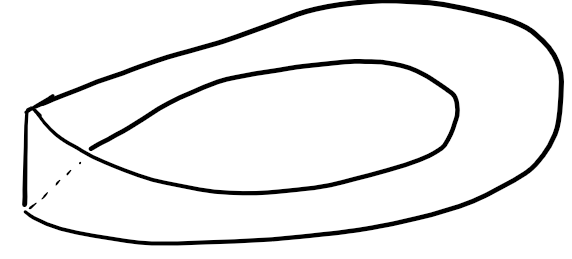
\includegraphics[width=60mm]{Images/mobius}
\caption{A (bad?) drawing of a M\"obius strip}
\label{fig-Mob} 
\end{figure}

\item \label{NO-surfaces} *Repeat problem \ref{ex-this} the \href{https://en.wikipedia.org/wiki/Klein_bottle}{Klein bottle} and \href{https://en.wikipedia.org/wiki/Real_projective_plane}{real projective plane} as well. 

\item *If you are wondering where surface integral notion that looks like the notation \[\int_C f\,dx+g\,dy\] of line integrals is, it's technically buried in the expression \eqref{Surface-vf}. The problem is, the ``thing'' we have to integrate over $S$ is called a \textit{2-form} (more generally a type of differential form). We benefit from differential forms simplifying to easier to parse equations like \eqref{Surface-vf} for dimensions 2 and 3, but this is not the case more generally. 

Suppose we have a surface $S$ parametrized by $r(u,v)=(x(u,v), y(u,v), z(u,v))$. Let us define the following \textit{wedge products} of differentials
\[ 
	dx\wedge dy= \det \begin{pmatrix} x_u  & x_v \\ y_u & y_v \end{pmatrix}dA ,\quad  
	dy\wedge dz= \det \begin{pmatrix} y_u  & y_v \\ z_u & z_v \end{pmatrix}dA, \quad 
	dx\wedge dz= \det \begin{pmatrix} x_u  & x_v \\ z_u & z_v \end{pmatrix}dA
	\]
where $dA$ is a placeholder for either $du\,dv$ or $dv\,du$.
\begin{enumerate}
	\item Show that $dy\wedge dx=-dx\wedge dy$. (Note: this also shows $dz\wedge dy=-dy\wedge dz$ and $dz\wedge dx=-dx\wedge dz$)
		
	\item Use part a. along with \eqref{Surface-vf} to show that if $F=(f,g,h)$ is a given vector field in $\mathbf{R}^3$ then 
	
	\[ \iint_{S} f \, dy\wedge dz + g\, dz\wedge dx+h \, dx\wedge dy =\iint_{S} F\cdot d\vec{n} \] 
\end{enumerate}
\end{enumerate}

Suggested additional exercises: \textit{Stewart} sections 16.6, 16.7


\section{Curl and divergence}

We now introduce the terminology of \textit{curl} and \textit{divergence} as vector field operations for vector fields in $\mathbf{R}^3$. 


Recall that for a scalar function $f=f(x,y)$ we have $\nabla f=(f_x,f_y)$ (similarly with three variable functions, etc.). Said differently, $\nabla$ assigns vector field to each scalar function so can be thought of as a ``function whose domain is functions''\footnote{This is still technically a function, but sometimes we use the word \textit{operator} for this kind of thing}. \[ \nabla \colon \text{ \{scalar functions of $n$ variables\} } \to \text{ \{vector fields in $\mathbf{R}^n$\} } \]
Once a dimension is fixed (for instance, $n=3$) it is helpful to think of  $\nabla$ as the ``symbolic vector'' \begin{equation}\label{grad} \nabla = \left( \dfrac{\partial}{\partial x} \, , \dfrac{\partial}{\partial y}\, , \dfrac{\partial}{\partial z}\, \right) \end{equation} 

\subsection{Curl of a vector field in $\mathbf{R}^3$}
\begin{defn}[Curl of a vector field in $\mathbf{R}^3$] The \textbf{curl} of a vector field $F=(f,g,h)$ in $\mathbf{R}^3$ is defined as follows. 
\begin{equation} \label{curl} \curl F = ( h_y-g_z, f_z-h_x, g_x-f_y)\end{equation}
\end{defn}

\begin{remark}
	The equation \eqref{curl} is obviously a bit opaque at first, but there's a much better way of thinking about it. Let's let $F=(f,g,h)$ be a vector field on $\mathbf{R}^3$, then \begin{equation}
		\curl F= \nabla \times F = \det \begin{pmatrix} \vspace{2mm} \vec{i} & \vec{j} & \vec{k} \\ \vspace{2mm} \dfrac{\partial}{\partial x} & \dfrac{\partial}{\partial y}  &\dfrac{\partial}{\partial z} \\ f & g & h\end{pmatrix}
	\end{equation}


 In the most general sense, $\curl F$ calculates the \textbf{instantaneous rotation} of $F$ at a point in its domain. What's maybe not clear at first is that rotations in $\mathbf{R}^3$ must occur about an axis\footnote{This is intuitive but maybe not known explicitly: it follows from \href{https://en.wikipedia.org/wiki/Euler\%27s_rotation_theorem}{Euler's rotation theorem} and is generally reflected in the \href{https://en.wikipedia.org/wiki/3D_rotation_group}{``rotational structure''} of $\mathbf{R}^3$.}. 

To reemphasize, $\curl F$ is a \textit{vector}, so it has a direction and magnitude. Let's write out what these do. At a point $P$ in $\mathbf{R}^3$:
\begin{itemize}
	\item The \textbf{direction} of $\curl F$ is the normal vector to the plane of rotation for the vector field at the point $P$. This normal direction is taken in accordance with the \textit{right hand rule} (i.e., if your right-hand fingers go in the direction of the rotation, the thumb points in the direction of the normal vector).
	\item The \textbf{magnitude} of $\curl F$ is proportional to the ``amount'' of rotation\footnote{Physically you can think of this as angular velocity, mathematically, this is the limiting ratio of $\oint_C F\cdot d\vec{r}$ and the arclength of $C$ for $C$ a small loop around $P$ in the plane of rotation going \textit{with} the rotation of $F$.}
\end{itemize}
Note that the $z$-component of $\curl F$ is the same quantity from Green's theorem and for testing conservativeness of a vector field $F=(f,g)$ (this is not a coincidence, we'll see why later). What $\curl$ computes for us is the ``instantaneous circulation'' of a given vector field about a point in $\mathbf{R}^3$--for instance, if a vector field ``rotates'' within some plane, the curl will point in a direction perpendicular to that plane (with direction given by the right hand rule).
\end{remark}

\begin{thm}[Conservative vector fields are curl-free] If $F$ is a vector field defined on $\mathbf{R}^3$ with $\curl F=0$ then $F$ is conservative (i.e., $F=\nabla \varphi$) for some scalar function $\varphi$. 
\end{thm}
That $F$ be defined on $\mathbf{R}^3$ is sufficient, but overkill for this theorem. Recall we had a similar theorem for vector fields in $\mathbf{R}^2$, wherein the requirement was that the domain of $F$ be \textit{simply connected}. That's still the case, but it's often not so ``obvious'' to tell when a region in $\mathbf{R}^3$ is simply connected\footnote{For instance, the domain $\mathbf{R}^3$ with a point removed \textit{is} simply connected, but $\mathbf{R}^3$ with an (infinite) \textit{line} removed is not---can you tell why?}.


\subsection{Divergence of a vector field}
\begin{defn}[Divergence of a vector field in $\mathbf{R}^3$] Let $F=(f,g,h)$ be a vector field in $\mathbf{R}^3$, the \textbf{divergence} of $F$---written $\dv F$---is the scalar function given by \begin{equation} \label{div} \dv F =\nabla \cdot F= f_x+g_y+h_z \end{equation}
\end{defn}

In some sense, divergence is the dual operation to taking the gradient of a scalar function. In particular, the output $\dv F$ is always a scalar function. Note as well, that the dimension is not important here, the  divergence is defined for a vector field in any dimensional space in a similar way: $\dv F=\nabla \cdot F$ for $F$ a vector field on $\mathbf{R}^n$. 


Divergence measures the tendency of a vector field $F$ to ``emerge'' from (i.e., go in to or come out of) some given point. That is, if $F$ is a vector field and $P$ a point in its domain, then\begin{itemize}
	\item $\dv F(P)>0$ means that $F$ is \textit{emerging from} the point $P$. We  call such a  point a \textbf{source}.
	\item $\dv F(P)<0$ means that $F$ is \textit{going into} the point $P$. We  call such a point a  \textbf{sink}.
	\item $\dv F(P)=0$ means that $F$ neither emerges from or goes into $P$. A vector field $F$ for which $\dv F$ is always $0$  is called \textbf{incompressible}\footnote{This is evidently an adopted word from fluid mechanics: A \textit{flow} of a fluid can be  \href{https://en.wikipedia.org/wiki/Incompressible_flow}{\textit{incompressible}} (which is slightly different than the fluid itself being incompressible)}. 
\end{itemize}

\begin{example}
	We've already seen an example of divergence. Recall the flux form of Green's theorem: if $F=(f,g)$ is a vector field in $\mathbf{R}^2$ and $C$ is a closed simple curve bounding region $R$ then \begin{equation} \int_C F\cdot d\vec{n}=\iint_R (f_x+g_y)\,dA\end{equation}
The right-hand side is just the divergence of the vector field $F$. In particular, the above is the 2D case of a more general theorem, \textit{The divergence theorem} (see section \ref{div-thm-sec}).
\end{example}

\subsection{Relationship between gradient, curl and divergence} 

Divergence, gradient and curl have some relations among them. A nice way of remembering it is as follows:
\[ \binom{\text{scalar functions}}{\text{on $\mathbf{R}^3$}} \xrightarrow{\nabla} 
\binom{\text{vector fields}}{\text{on $\mathbf{R}^3$}} \xrightarrow{ \curl} 
\binom{\text{vector fields}}{\text{on $\mathbf{R}^3$}} \xrightarrow{\dv} 
\binom{\text{scalar functions}}{\text{on $\mathbf{R}^3$}}  \]
Such that any chain of two successive is always $0$, i.e. for any scalar function $\varphi\colon\mathbf{R}^3\to \mathbf{R}$ and any vector field $F$ on $\mathbf{R}^3$  \[\curl (\nabla\varphi )=\vec{0} \qquad  \text{and} \qquad \dv (\curl  F)=0.\]



\subsection{Exercises}
\begin{enumerate}[label=\arabic*.]


\item Calculate $\curl F$ and $\dv F$ for the following vector fields $F$. Are any of these vector fields conservative?

\begin{enumerate}
	\item $F=(xy^2z^2, x^2y, xy^2)$
	\item $F=(1, xye^z, 2x-z)$
	\item $F=(\arctan(xy), xy, 1)$
\end{enumerate}

\item Let $F$ be a vector field on $\mathbf{R}^3$ and $g$ be some scalar function of three variables. Determine if the following expressions are vectors, scalars, or nonsense. 

\begin{enumerate}
	\item $\curl g$
	\item $(\curl F) \times (\nabla g)$
	\item $\dv (\dv F)$
	\item $\dv (\nabla g)$
	\item $\nabla(\dv F)$
	\end{enumerate}
	
	\item Show that if $\varphi$ is a scalar function of $3$ variables then $\curl(\nabla \varphi)=(0,0,0)$. Similarly, show if $F$ is a vector field on $\mathbf{R}^3$ then $\dv(\curl F)=0$. (Assume $\varphi$ and $F$ have continuous second-order partial derivatives)

\item Use the ``symbolic operator'' interpretation of $\nabla$ from \eqref{grad} to show that $\curl F= \nabla \times F$ and $\dv F= \nabla \cdot F$ for $F$ a vector field in $\mathbf{R}^3$.

\item  Let $F,G$ be a vector fields on $\mathbf{R}^3$ and $g$ some scalar function of three variables. Show the following identities:

\begin{enumerate}
	\item $\dv (gF)=g \,\dv F + F\cdot \nabla g$
	\item $\dv (F\times G)=G \cdot \curl F - F \cdot \curl G$
	\item $\curl( \curl F)=\nabla (\dv F) - \nabla^2 F$\footnote{Here, $\nabla^2 g= g_{xx}+g_{yy}+g_{zz}$ is the \textit{Laplace operator} and if $F=(f,g,h)$ then \[\nabla^2 F= (\nabla^2 f, \nabla^2 g, \nabla^2 h)\]}  

\end{enumerate}



\item Let $F$ be the inverse square field \[ F(x,y,z)=\left( \dfrac{x}{(x^2+y^2+z^2)^{3/2}}, \,\dfrac{y}{(x^2+y^2+z^2)^{3/2}} , \,\dfrac{z}{(x^2+y^2+z^2)^{3/2}} \right) \] 
Show that $\dv F=0$. Is there a vector field $G$ such that $F=\curl G$?
\end{enumerate}
Suggested additional exercises: \textit{Stewart} section 16.5


\section[Stokes' and Divergence theorem]{Stokes' theorem and Divergence theorem}

In $\mathbf{R}^2$ we saw the two forms for Green's theorem. For a vector field $F$, and closed simple curve $C$ bounding region $R$ in $\mathbf{R}^2$ these statements can be summarized as
\begin{itemize}
	\item The \textit{circulation} of $F$ over $C$ equals the integral of the \textit{(2D) curl} of $F$ over $R$ (theorem \ref{thm-green})
	\item The \textit{flux} of $F$ over $C$ equals the integral of the \textit{divergence} of $F$ over $R$ (corollary \ref{green-flux})
\end{itemize}
In this last section, we'll learn the appropriate 3D analogs to these two statements. 

One of the complexities of $\mathbf{R}^3$ vs $\mathbf{R}^2$ is that the appropriate analogs of these two statements apply to different types of regions. The correct generalization of the classic form of Green's theorem (the circulation form \ref{thm-green}) is Stokes' theorem (theorem \ref{thm-stokes}); for the flux form of Green's theorem, the correct generalization is the Divergence theorem (theorem \ref{thm-divergence}). 

\subsection{Stokes' theorem}
Let $C$ be a closed, simple, oriented curve in $\mathbf{R}^3$ and $S$ some surface whose boundary is $C$. Then, for $F$ a vector field in $\mathbf{R}^3$, the \textit{circulation} of $F$ over the curve $C$ is equal to the curl of $F$ integrated over $S$. There's a subtlety here in that $\curl F$ is a vector field, so it's really the \textit{flux} of this vector field $\curl F$ through that is being calculated. 

\begin{figure}[h!]
\centering
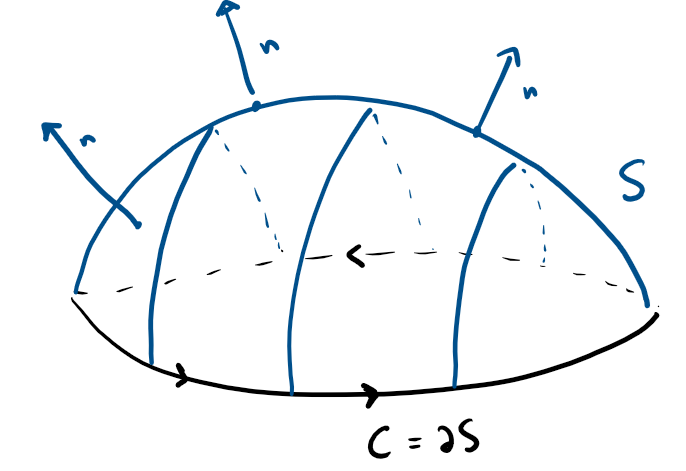
\includegraphics[width=70mm]{Images/surface-stokes}
\caption{A consistent choice of orientation on $S$ and $C=\partial S$ for Stokes' theorem}
\label{fig-stokes-thm}
\end{figure}

\begin{thm}[Stokes' theorem] \label{thm-stokes} Let $S$ be an oriented surface in $\mathbf{R}^3$ with boundary curve $\partial S = C$ oriented positively. If $F$ is a vector field in $\mathbf{R}^3$ such that all first-order partial derivatives of $F$ exist and are continuous on $S$ then
\begin{equation}
	\oint_C F\cdot d\vec{r}= \iint_{S} \curl F \cdot d\vec{n}
\end{equation}
\end{thm}

As with the other theorems we've learned it's good to start with an entirely superficial analysis: the left hand side is a \textbf{line integral} of a vector field over a curve; the right hand side is a \textbf{surface integral} of the vector field $\curl F$. Everything involved should have three components. 


\begin{remark} The relationship between $S$ and its boundary $\partial S=C$ is the most nuanced for Stokes' theorem. Both $S$ and $C$ need to be oriented, and their orientations need to agree. The easiest way to think about it is like this: Give $C$ an orientation, there is then an induced orientation on $S$ via the ``right-hand rule'' (i.e., your right hand fingers point in the direction of $C$, the thumb points in the direction of normality to $S$). Conversely, given an orientation on $S$ you can reverse engineer the appropriate orientation on $C$. See Figure \ref{fig-stokes-thm}.


\end{remark}

%subsection{Gradient, curl, and divergence operations} 
%Moreover, Stokes' theorem (unlike the Divergence theorem) is specific to $\mathbf{R}^3$. There is also a more general theorem (also called \href{https://en.wikipedia.org/wiki/Generalized_Stokes_theorem}{Stokes' theorem}) which implies all of the vector calculus theorems we've learned: FTC for line integrals, Green's theorem, Divergence theorem, and Stokes' theorem. The general idea here is that the operations: \textbf{gradient}, \textbf{divergence}, and \textbf{curl} are all ``derivative-like'' operations, and that integrating the ``derivative'' of something over a region $R$ will always be the same as integrating the thing over the boundary $\partial R$ (see Ap. \ref{brief}).



\subsection{The divergence theorem}\label{div-thm-sec}

The \textit{Divergence theorem}\footnote{Sometimes also called \textit{Gauss' theorem}.}  applies whenever we have a solid region $R$ in $\mathbf{R}^3$ with boundary $S$, and relates the \textit{flux} of $F$ through $S$ to the triple integral over $R$ of the divergence of $F$. 
\begin{figure}[h!]
\centering
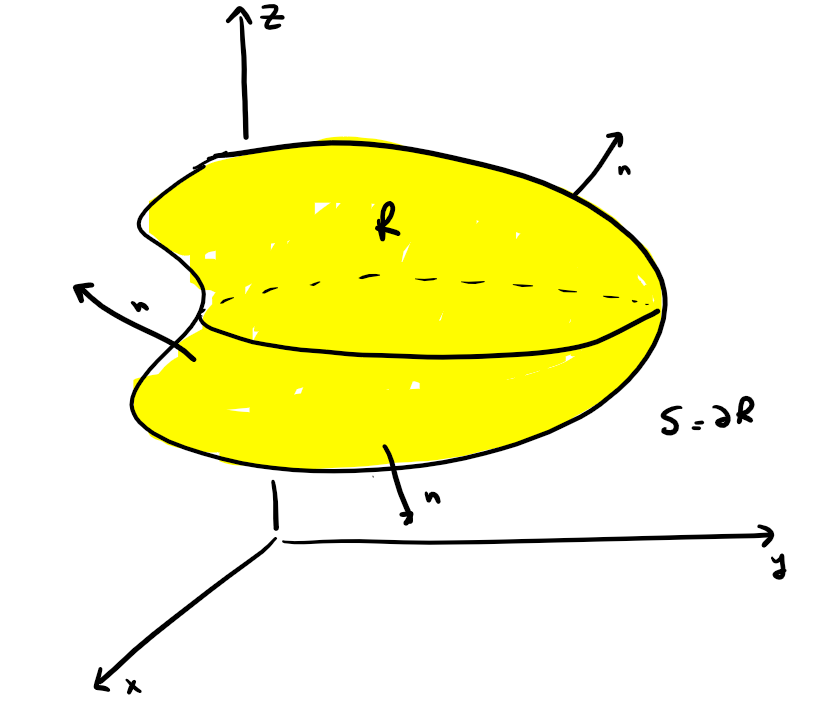
\includegraphics[width=80mm]{Images/region-div-thm}
\caption{An (outward) oriented closed surface $S$ which bounds a region $R$ in $\mathbf{R}^3$}
\label{fig-region-div-thm}
\end{figure}

\begin{thm}[Divergence theorem]\label{thm-divergence} Let $R$ be a simple solid region in $\mathbf{R}^3$ and let $S=\partial R$ be the boundary of $R$ with positive orientation (i.e., normal vector points outward). If $F$ is a vector field on $\mathbf{R}^3$ such that the first-order partial derivatives of all component functions of $F$ exist and are continuous on all of $R$, then:
\begin{equation} \label{div-thm}
	\iint_{S} F\cdot d\vec{n}= \iiint_R \dv F \,dV 
\end{equation}
\end{thm}

\begin{remark} Let's piece together some of the features of this theorem
\begin{itemize}
\item The left-hand side of the Divergence theorem is the \textit{flux} through the surface (with positive orientation). With this interpretation you can think of $\dv F$ as ``flux density'' on the enclosed region $R$. 



 \item It's not immediately clear, but is generally true for the surface $S=\partial R$ in \eqref{div-thm} that $\partial R$ must be \textbf{closed} (i.e., $\partial R$ itself has no boundary\footnote{Note more generally that the boundary of the boundary of a solid region, surface, etc. is always empty. This is sometimes written algebraically as $\partial^2=0$}.). So, in mirroring notation from line integrals, you'll sometimes see \[ \oiint_{\partial R} F\cdot d\vec{n}\] to emphasize this feature of $\partial R=S $. Again, the symbol $\displaystyle \oiint$ means the same thing as $\displaystyle \iint$, it just emphasizes that the region of integration is closed. 

\item Like Green's theorem, the Divergence theorem applies to only certain types of domains $R$. The exact definition of \textit{simple solid region in $\mathbf{R}^3$} is perhaps a bit subtle (see also def. \ref{def-solid-region}), but can most easily be thought of a solid chunk bounded by some collection of (non-degenerate) surfaces. For example, the solid ball $x^2+y^2+z^2\leq 1$ is bound by the sphere $x^2+y^2+z^2=1$. 
\end{itemize}
\end{remark}

 The Divergence theorem is \textit{not} specific to $\mathbf{R}^3$. In $\mathbf{R}^2$, we've seen how Green's theorem can be modified to give a ``Divergence theorem" in $\mathbf{R}^2$. More generally, the Divergence theorem phenomenon exists in all dimensions with the appropriate understanding of ``hypersolid enclosed by a hypersurface''.



%\subsection{The Laplacian and diffusion}Divergence is also related to the \textit{Laplacian} of a function \begin{equation} \nabla^2 f= \nabla \cdot (\nabla f)\end{equation} for $f$ a scalar function of $n$ variables. This operator $\nabla^2$ is used quite often in physics, as it is a good model for diffusion of a quantity through space\footnote{For instance, you see this in the \href{https://en.wikipedia.org/wiki/Heat_equation}{heat equation}, the \href{https://en.wikipedia.org/wiki/Wave_equation}{wave equation}, and \href{https://en.wikipedia.org/wiki/Schr\%C3\%B6dinger_equation}{Schr\"odinger's equation}.}.


\subsection{Exercises}
\begin{enumerate}[label=\arabic*.]

\item Use Stokes' theorem to evaluate $\displaystyle \iint_{S} \curl F\cdot d\vec{n}$ for the following:

\begin{enumerate}
	\item $F=(x^2\sin z, y^2, xy)$, $S$ the portion of $z=1-x^2-y^2$ with $z\geq 0$ oriented upward. 
	\item $F=(xyz, xy, x^2yz)$, $S$ the four sides and top of the cube with vertices $(\pm 1, \pm 1, \pm 1)$, but not the bottom face, oriented outward
\end{enumerate}

\item Use Stokes' theorem to evaluate $\displaystyle \oint_C F\cdot d\vec{r}$ for the following:

\begin{enumerate}
	\item $F=(x+y^2, y+z^2, z+x^2)$, $C$ the triangle with vertices $(0,0,1), (0,1,0)$ and $(1,0,0)$ oriented counterclockwise in the $xy$-plane. 
	\item $F=(ze^x, z-y^2, x-z^3)$, $C$ the circle given by $y^2+z^2=4$ and $x=3$ oriented counterclockwise when viewed from the origin. 
	\item $F=(x^3-z, xy, y+z^2)$,  $C$ the intersection of $z=x^2+y^2$ and $z=x$ oriented clockwise when projected into the $yz$-plane. 

\end{enumerate}

\item Explain why if $S$ is a sphere and $F$ satisfies the condition of Stokes' theorem that \[\iint_{S} \curl F\cdot d\vec{n}=0\]
\item \label{stokes-greens} Let $f=f(x,y), g=g(x,y)$ be differentiable scalar functions. Show that Stokes' theorem gives Green's theorem when applied to the vector field $F=(f,g,0)$ and $S$ is a region of the $xy$-plane.

\item Let $E$ and $B$ represent electric and magnetic fields respectively. Faraday's observation was that an electric current is produced by varying a magnetic field in a closed loop. Said differently, if $S$ is an oriented surface, then $B$ induces an electric field which satisfies \[\oint_{\partial S} E\cdot d\vec{r}= -\iint_{S} B_t \cdot d\vec{n}\] (\textit{Note: $B_t$ represents the time derivative of $B$}.) What does this tell you about the relationship between $E$ and $B$ in relation to curl?\footnote{Can you now parse the other three of \href{https://en.wikipedia.org/wiki/Maxwell\%27s_equations\#Macroscopic_formulation 
}{Maxwell's equations}?}

\item Use the Divergence theorem to calculate the flux of the vector field $F$ across the given surface.

\begin{enumerate}
	\item $F=(xy, xy^2, e^{xy})$, $S$ the box bounded by the coordinate planes and planes $x=3, y=2, z=1$. 
	\item $F=(xe^y, z-e^y, -xy)$, $S$ the ellipsoid $x^2+2y^2+3z^2=4$.
	\item $F=(xy+2xz, x^2+y^2, xy-z^2)$, $S$ the solid cylinder bound by $x^2+y^2=4$ and planes $z=0, z=2$.
	\item $F=(z,y,zx)$, $S$ the tetrahedron bounded by plane $x+y+z=1$ in the first octant. 
	\item $F=(x^2z,xz^2, y\ln(x+1))$, $S$ the wedge in the first octant bound by $x+2z=4$ and $y=3$
\end{enumerate}

\item  Let $R$ be a simple solid region in $\mathbf{R}^3$. Use the Divergence theorem to show the following identities: 

\begin{enumerate}
	\item $\displaystyle \oiint_{\partial R} F\cdot d\vec{n}=0$ for $F$ any constant vector field
	\item $\displaystyle \text{Volume of $R$} = \dfrac{1}{3} \oiint_{\partial R} (x,y,z)\cdot d\vec{n}$\\
	\item $\displaystyle \oiint_{\partial R} \curl F\cdot d\vec{n}=0$ for all vector fields $F$. (\textit{Hint: what is the relation between curl and divergence?})

\end{enumerate}



\item Let $F$ be the vector field in $\mathbf{R}^2$ given below
\[ 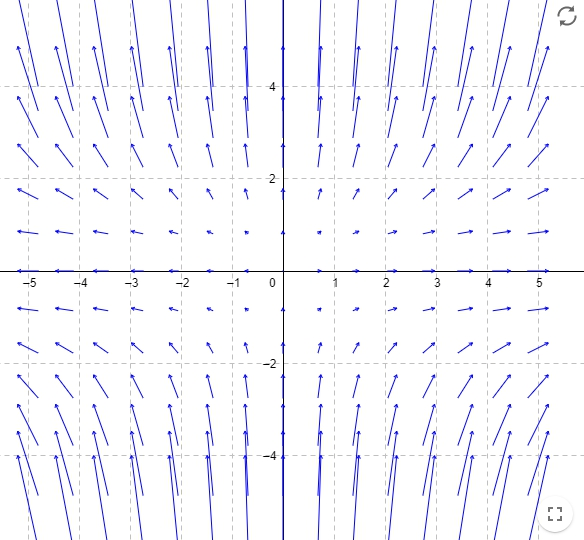
\includegraphics[height=60mm]{Images/ws14-vf}\]
Plot a point  $P$ (or explain why no such point exists) such that \begin{enumerate}
\item $\dv F(P)>0$
\item $\dv F(P)<0$
\item $\dv F(P)=0$
\end{enumerate}



\item  *One neat corollary to the Divergence theorem is that the divergence of $F$ itself can be computed by the limiting value of flux over certain surface integrals. Let $B_r$ be the solid ball of radius $r$ centered at some point $(a,b,c)$ in $\mathbf{R}^3$ and $S_r$ the bounding sphere. Show the following: \[ (\dv F) (a,b,c) = \lim_{r\to 0^+} \dfrac{1}{\text{volume of $B_r$}} \oiint_{S_r} F\cdot d\vec{n}\] 
\end{enumerate}
Suggested additional exercises: \textit{Stewart} sections 16.8, 16.9

\appendix


\section[Vector calculus summary]{A brief summary of vector calculus in $\mathbf{R}^2$ and $\mathbf{R}^3$}

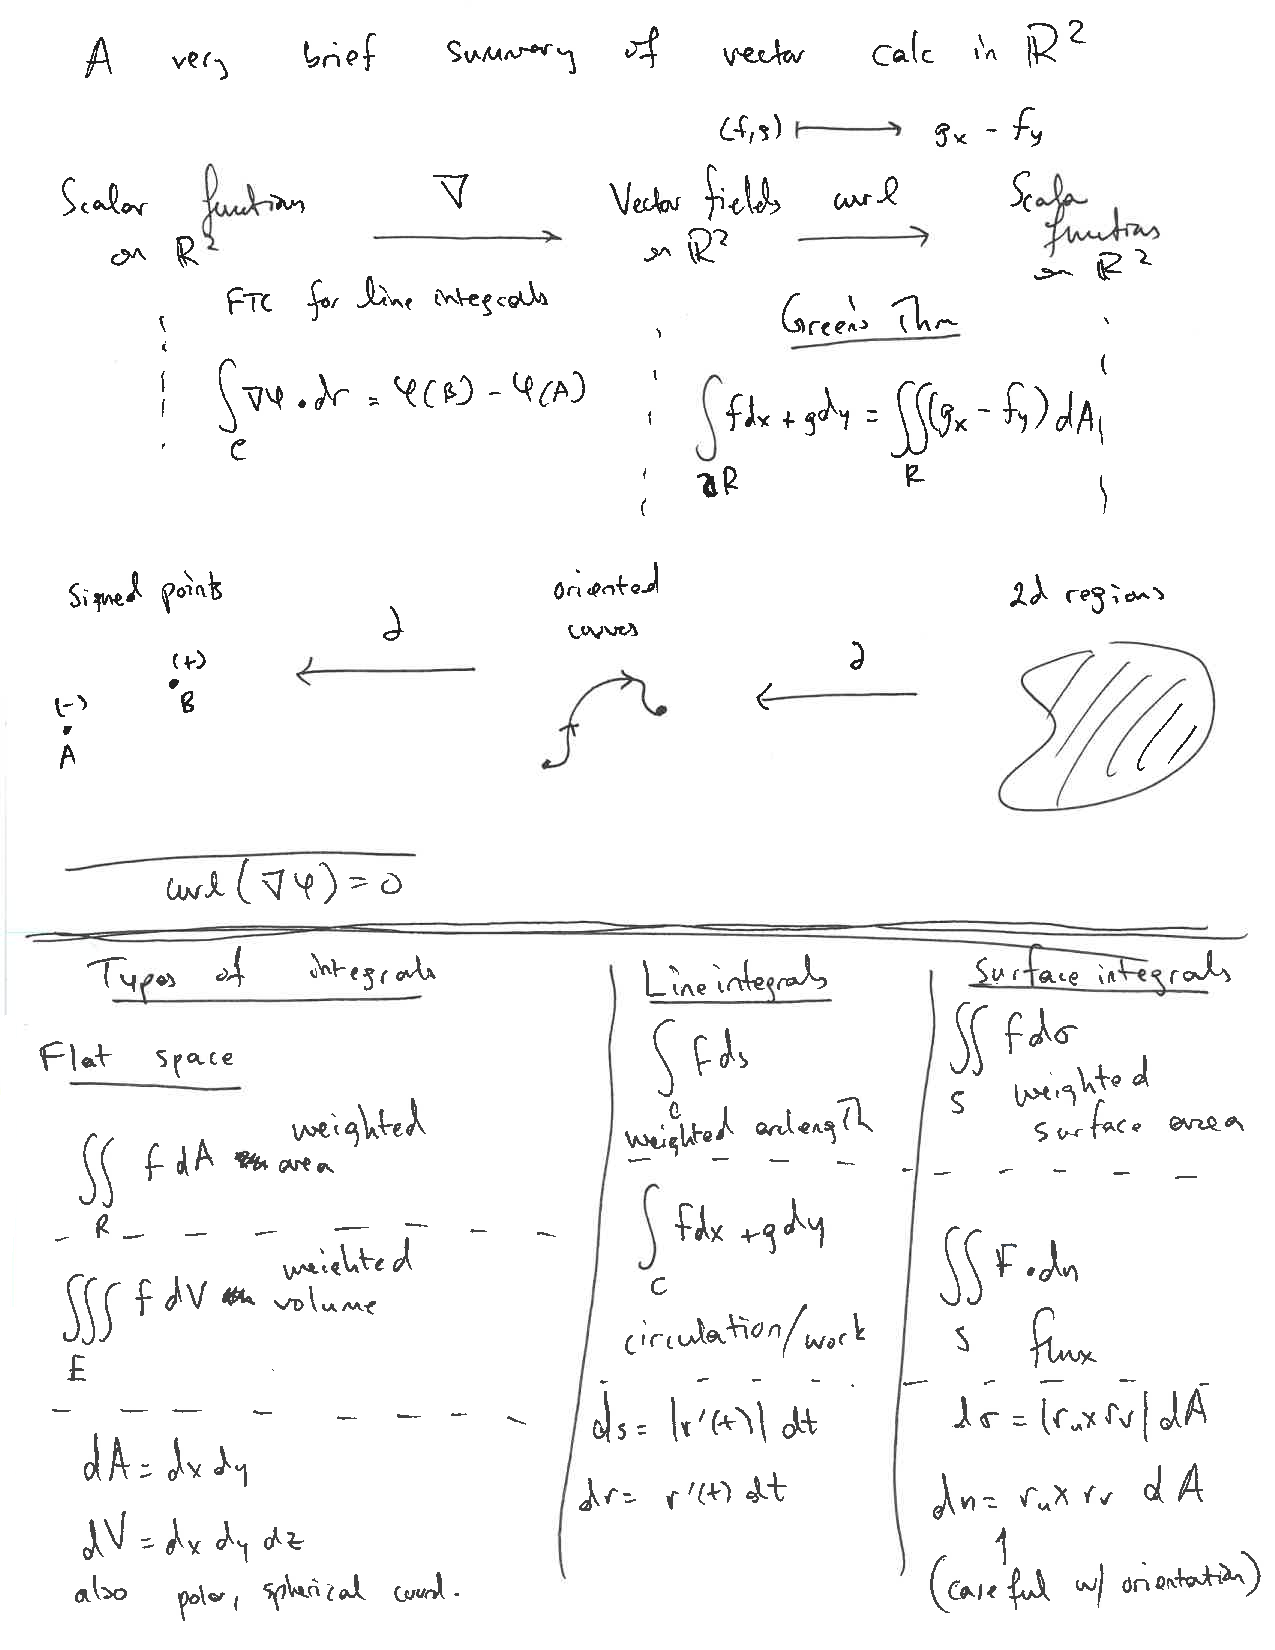
\includegraphics[width=7in]{Images/r2}



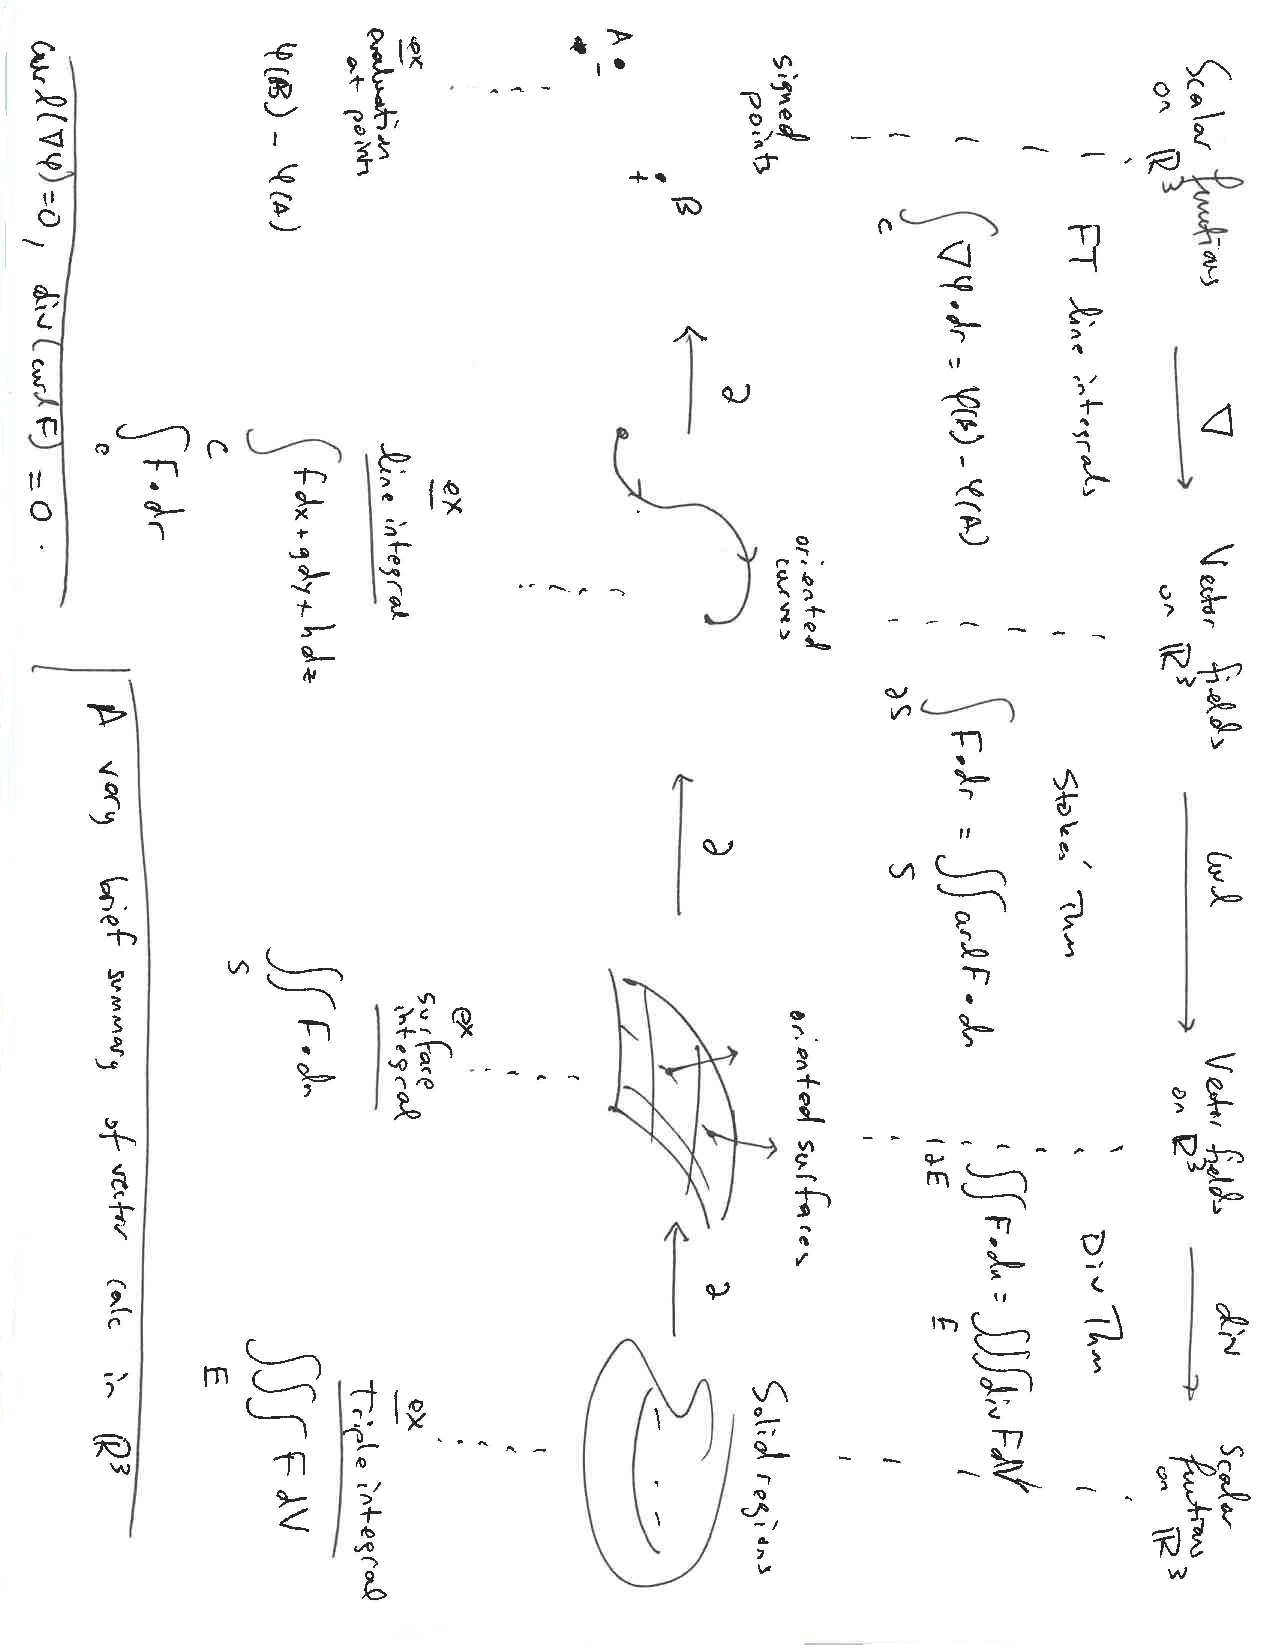
\includegraphics[width=7in]{Images/r3}

\end{document}
\newpage

\[
\begin{tikzcd}
	\binom{\text{Functions}}{\R^3\to\R} \arrow{rr}{\nabla} \arrow{dd}
	&& \binom{\text{Vector fields}}{\text{on $\R^3$}} \arrow{rr}  \arrow{dd}
	&&\binom{\text{Vector fields}}{\text{on $\R^3$}} \arrow{rr} \arrow{dd}
	&&\binom{\text{Functions}}{\R^3\to\R} \arrow{dd}\\
	& \varphi(B)-\varphi(A)=\int_C F\cdot d\vec{r}
	&& \int_{\partial D} F\cdot d\vec{r}=\iint_D \curl F\cdot d\vec{n}
	&& \text{Divergence Theorem}\\
	\text{Signed points} 
	&& \text{Oriented curves}
	&& \text{Oriented surfaces}
	&& \text{3D solid regions}
\end{tikzcd}
\]
\end{landscape}


\newpage
\appendix


\section{Exam reviews} 

\newpage

\section{Coordinate substitutions}

\subsection{Polar coordinates} Conversion from $(x,y)$ to polar coordinates $(R,\theta)$
		\begin{itemize}
			\item[] $x=R\cos \theta$
			\item[] $y=R\sin \theta$
			\item[] $R^2=x^2+y^2$
			\item[] $dA=R d\vec{r}\,d\theta$\\
		\end{itemize}


\subsection{Spherical coordinates}
The sphere $x^2+y^2+z^2=\rho^2$ is parametrized by $r(\theta, \varphi)$ which has $x,y,z$ components given by: 
\begin{itemize}
	\item $x=\rho \cos \theta \sin \varphi$
	\item $y=\rho \sin \theta \sin \varphi$
	\item $z=\rho \cos \varphi$\\
	
	For this coordinate transformation, you may freely use the following
	\item $dV= \rho^2\sin \varphi \,d\rho\,d\varphi\,d\theta$
	\item $n=\pm \, r_{\theta} \times r_{\varphi}=\pm \,(\rho^2 \cos \theta \sin^2 \varphi, \rho^2 \sin \theta \sin^2\varphi, \rho^2 \sin \varphi \cos \varphi)$
	\item $|r_{\theta}\times r_{\varphi}| = \rho^2 \sin\varphi$.\\
	\end{itemize}




\newpage



\newpage



















\end{document}











